\documentclass[a4paper]{jarticle}

%必要なパッケージを追加する
%\usepackage{docmute}
%\usepackage{caption}
%\usepackage[subrefformat=parens]{subcaption}
%\usepackage[dvipdfmx]{graphicx}
%\usepackage{longtable} % 長い表生成用
%\usepackage{texilikecover} % 表紙のデザイン用
%\usepackage{listliketab}
%\usepackage{ascmac}
%\usepackage{comment}
%\usepackage{here}
%\usepackage{mediabb}
%以上は追加済み

\usepackage{docmute}
\usepackage{caption}
\usepackage[subrefformat=parens]{subcaption}
\usepackage[dvipdfmx]{graphicx}
\usepackage{longtable} % 長い表生成用
\usepackage{texilikecover} % 表紙のデザイン用
\usepackage{listliketab}
\usepackage{ascmac}
\usepackage{comment}
\usepackage{here}
\usepackage{mediabb}


% --*- coding:utf-8-unix mode:latex -*--
% Beginファイル

\usepackage{docmute}
\usepackage{caption}
\usepackage[subrefformat=parens]{subcaption}
\usepackage[dvipdfmx]{graphicx}
\usepackage{longtable} % 長い表生成用
\usepackage{texilikecover} % 表紙のデザイン用
\usepackage{listliketab}
\usepackage{ascmac}
\usepackage{comment}
\usepackage{here}
\usepackage{mediabb}


% 文書の表示領域指定
\headsep -10mm
\oddsidemargin -0mm
\textwidth 160mm
\textheight 240mm

% 文書の設定
\setcounter{secnumdepth}{6}  %小節番号の付番レベル

% 表紙
\title{平成31年度新入生歓迎セミナー企画書}
\group{高知工科大学 情報学群}
\version{8.0}
\author{
	\begin{tabbing}
		1234567\=890\kill
		代表\>:
		宮尾 将史\\
		{\large Mail}\>
		{\large : 210379e@ugs.kochi-tech.ac.jp}\\
		{\large TEL}\>
		{\large : 090-4979-3142}\\\\
		副代表\>:
		東 聖\\
		{\large Mail}\>
		{\large : hazuma710@gmail.com}\\
		{\large TEL}\>
		{\large : 090-7788-7100}\\\\
		副代表\>:
		藤沢 元\\
		{\large Mail}\>
		{\large : 210362t@ugs.kochi-tech.ac.jp}\\
		{\large TEL}\>
		{\large : 080-8585-4634}
	\end{tabbing}
}

\begin{document}

\maketitle
\tableofcontents
\newpage
 %\documentclass[12pt]{jarticle}
\usepackage{docmute}
\usepackage{caption}
\usepackage[subrefformat=parens]{subcaption}
\usepackage[dvipdfmx]{graphicx}
\usepackage{longtable} % 長い表生成用
\usepackage{texilikecover} % 表紙のデザイン用
\usepackage{listliketab}
\usepackage{ascmac}
\usepackage{comment}
\usepackage{here}
\usepackage{mediabb}


%ここから上は触らない
%必要なパッケージを追加する
%\usepackage{docmute}
%\usepackage{caption}
%\usepackage[subrefformat=parens]{subcaption}
%\usepackage[dvipdfmx]{graphicx}
%\usepackage{longtable} % 長い表生成用
%\usepackage{texilikecover} % 表紙のデザイン用
%\usepackage{listliketab}
%\usepackage{ascmac}
%\usepackage{comment}
%\usepackage{here}
%\usepackage{mediabb}

%以上は追加済み

%\usepackage{}


\begin{document}
% 必要な項目ができた場合は適宜サブセクションを追加してください

% イベント名を記入する
%例:\section{大学到着後}
\section{sample}

% 日時と場所を記入する
% 時刻は4桁で記入すること!
\subsection{日時・場所}
\begin{tabular}{p{2zw}rp{38zw}}
	日時 & : & 2016年4月17日(日) 16:00 $\sim$\\ 
	場所 & : & 東ロータリー,K102
\end{tabular}


% イベントのタイムスケジュールを記入する
% 時刻は必ず4桁(00:00)で記入すること!
% 時間の流れは途切れないように記述する!
\subsection{タイムスケジュール}
\begin{longtable}{p{3zw}p{39zw}}
	16:00 & \textbf{◎ 工科大到着} \\\\
	
	16:15 & \textbf{◎ 新入生見送り終了} \\
	& \ \ \textbullet \ \ 新入生全員の解散の確認後,スタッフの荷物,その他物品をK102に全員で運ぶ \\\\
	
	16:20 & \textbf{◎ 教室移動後} \\
	& \ \ \textbullet \ \ ゴミを指定の場所へ捨てに行く\\
	& \ \ \textbullet \ \ 分別ができていないものは分別する\\
	& \ \ \textbullet \ \ 各研究室,個人,教務部から借りた物品が揃っていることを確認し,順次返却を行う(教務部への返却は多田,和田が行う)\\
	& \ \ \textbullet \ \ 返却先が不在等で返却できない場合,一時的に清水研究室にて荷物を保管しておき,後日代表陣が物品の返却を行う\\\\
	
	16:40 & \textbf{◎ 反省会} \\\\
	
	17:00 & \textbf{◎ 解散!!} \\  
\end{longtable}

\subsection{人員配置}
%例:教務部への物品返却:多田,和田

% イベントに必要な物品と個数を記入する
% 記入例 ・マジックペン 10本
\subsection{必要物品}

% 注意事項やスタッフに周知しておくべきことがあれば記入する
\subsection{備考}

\end{document}
% 必要な項目ができた場合は適宜サブセクションを追加してください

%\include{begin}
% イベント名を記入する
\section{当日準備}


% 日時と場所を記入する
% 時刻は4桁で記入すること!
\subsection{日時・場所}
\begin{tabular}{p{2zw}rp{38zw}}
  日時 & : & 2019年4月5日(金) 07:00 $\sim$ 10:30\\ %時間を確認してください
  場所 & : & K101, A109                                        %教室を確認する
\end{tabular}

% 目的を記入する
\vspace{-5mm}
\subsection{目的}
準備物や自分の役割の最終確認をする

% イベントのタイムスケジュールを記入する
% 時刻は必ず4桁(00:00)で記入すること!
% 時間の流れは途切れないように記述する!
\vspace{-5mm}
\subsection{タイムスケジュール}
\begin{longtable}{p{3zw}p{39zw}} %詳細が決まり次第作業

  $\sim$06:00 & \textbf{◎ 各自起床} \\
        & \ \  \textbullet \ \ 遅刻しそうな人は報告slackに連絡する \\
        & \ \  \textbullet \ \ 互いにモーニングコールをかけ合おう \\\\

  07:00 & \textbf{◎ 集合部屋(A109)に集合} \\
  	    & \ \  \textbullet \ \ 朝礼挨拶をする \\
        & \ \  \textbullet \ \ 出席を確認する \\
        & \ \  \textbullet \ \ 遅刻者への連絡 \\
        & \ \  \textbullet \ \ 到着した人から自分の荷物にタグを付ける \\
        & \ \  \textbullet \ \ スタッフの参加費を代表者が集める \\\\

  07:10 & \textbf{◎ 1日目読み合わせ確認} \\
  	    & \ \  \textbullet \ \ 各自,印刷した企画書最新版で読み合わせを行う \\
        & \ \  \textbullet \ \ 各自が自分の役割を把握し,不明な点を解消する \\
        & \ \  \textbullet \ \ 同じ水準の知識を共有する \\
        & \ \  \textbullet \ \ 物品の確認を行う \\\\

  08:10 & \textbf{◎ 2日目読み合わせ確認} \\
        & \ \  \textbullet \ \ 1日目同様,読み合わせを行う \\
        & \ \  \textbullet \ \ 手の空いているスタッフは物品を再度確認する \\
        & \ \  \textbullet \ \ 確認後全体の記念撮影を部屋内(A109)で行う \\

  10:15 & \textbf{◎ 受け入れ用の部屋(K101:新入生, 先生)で受け入れ準備} \\
      	& \ \  \textbullet \ \ 受付,見回り,先遣隊,後遣隊,救護車がそれぞれに分かれて,準備にとりかかる \\\\

  10:30 & \textbf{◎ 受付準備開始} \\
\end{longtable}

% イベントに必要な役割と人数を記入する
% 担当者は決定次第追記する
% 記入例 ・司会者 2人(名前1,名前2)

% イベントに必要な物品と個数を記入する
% 記入例 ・マジックペン 10本
\subsection{必要物品}
\begin{itemize}
\item カメラ
\item スタッフ荷物用のタグ
\item 企画書
\end{itemize}

\subsection{備考}
企画書とタイムテーブルを印刷しておく

%\include{end}


% --*- coding:utf-8-unix mode:latex -*--
%\include{Begin}
%%%%%%%%%%%%%%%%%%%%%%%%%%%%%%%%%%%%%%%%%%%%%%%%%%%%%%%%%%%%%%%%%%%%%%%%%%%%%%%

\section{荷物の搬入}

\subsection{日時・場所}

\begin{tabular}{p{2zw}rp{38zw}}
  日時 & : & 2019年4月5日(金) 7:50$\sim$ 8:30\\
  場所 & : & K101, 東ロータリー
\end{tabular}

\subsection{目的}
迅速に荷物を運ぶ!!!!

\subsection{タイムスケジュール}
% 時刻は必ず4桁(00:00)で書くこと!!!
\begin{longtable}{p{3zw}p{39zw}}
   7:10 & \textbf{◎ 搬入開始} \\
        & \ \  \textbullet \ \ 小島,小松, 三浦, 西森は車を東ロータリーに停めておく \\
        & \ \  \textbullet \ \ K101から物品を車に積み込む \\\\

   7:20 & \textbf{◎ 物品確認} \\
        & \ \  \textbullet \ \ 先遣隊,後遣隊以外のスタッフはK101へ戻って読み合わせを始める \\
        & \ \  \textbullet \ \ 先遣隊,後遣隊は,本企画書と搬入した物品を確認する \\
        & \ \  \textbullet \ \ 物品がない場合は先遣隊が購入するためリストアップする \\
        & \ \  \textbullet \ \ 車が邪魔になりそうな場合は, 駐車場に移動させておく \\
        & \ \  \textbullet \ \ 西森は車を駐車場に移動させておく \\
        & \ \  \textbullet \ \ 出発準備が終わったら,出発時間までK101で読み合わせに参加する \\\\

   8:30 & \textbf{◎ 先遣隊出発} \\
        & \ \  \textbullet \ \ 忘れ物がないかよく確認する \\
        & \ \  \textbullet \ \ 横田が報告slackに連絡した後,出発する \\
\end{longtable}


\subsection{人員配置(人数により調整,運転者含む)}
\begin{itemize}
\item 先遣隊1:小島(車),宮尾
\item 先遣隊2:小松(車),横田
\item 先遣隊3:三浦(車),野田,以西

\end{itemize}

\subsection{備考}
\begin{itemize}
\item 前日までに荷物をK101へ運んでおく
\item 荷物は乗せる車ごとに分けておく
\item 研究室へ搬入の際にも物品を確認しておく
\item バス司会(塩谷, 中島, 丸田, 高橋(龍), 藤田(B3), 北村)はスタッフ集合部屋(K101)で酔い止めと水を受け取る
\end{itemize}


%%%%%%%%%%%%%%%%%%%%%%%%%%%%%%%%%%%%%%%%%%%%%%%%%%%%%%%%%%%%%%%%%%%%%%%%%%%%%%%
%\include{End}

% --*- coding:utf-8-unix mode:latex -*--
%\include{Begin}
%%%%%%%%%%%%%%%%%%%%%%%%%%%%%%%%%%%%%%%%%%%%%%%%%%%%%%%%%%%%%%%%%%%%%%%%%%%%%%%
\section{先遣隊}

\subsection{日時・場所}

\begin{tabular}{p{2zw}rp{38zw}}
  日時 & : & 2019年4月5日(金) 8:30 $\sim$ 15:30\\
  場所 & : & 工科大学 $\sim$ 国立幡多青少年自然の家
\end{tabular}

\subsection{目的}
本隊より先遣し国立幡多青少年自然の家に向かい,本隊が到着後円滑にセミナーが進行できるように事前準備を行う.


\subsection{タイムスケジュール}
% 時刻は必ず4桁(00:00)で書くこと!!!
\begin{longtable}{p{3zw}p{39zw}}

   8:30  & \textbf{◎ 出発} \\
        & \ \  ※休憩を取りながら向かう \\\\

  11:00 & \textbf{◎ 到着} \\
        & \ \  \textbullet \ \ 2台とも到着次第,横田が報告slackに連絡する \\\\

  11:10 %& \textbf{◎ 第一,第二集会室解錠(???)} \\
        %& \ \ \textbullet \ \ ?事務室から第一集会室と第二集会室の鍵,マイクをもらい,開錠を行う\\
        %& \ \ \textbullet \ \ ?なかよし広間とくろしお棟の鍵が開いているのかを室戸の職員さんに確認する\\
        %& \ \ \textbullet \ \ ?第一集会室と第二集会室を開錠次第,第一集会室の準備に加わる\\
        %& \ \ \textbullet \ \ ?第二集会室の鍵は荷物の詰め込みが終わり次第事務室に返却する\\
        %& \ \ \textbullet \ \ ?返却しなくてもよい場合,返却せずに鍵係が所持しておく\\\\

        & \textbf{◎ 打ち合わせ(ロビー)} \\ %部屋の鍵は全て開錠(10:00まで)
        & \ \ \textbullet \ \ 施設の方と最終的な打ち合わせを行い,変更点等があれば報告slackに連絡する \\
        & \ \ \textbullet \ \ 打ち合わせの際,入所式時に来てくださる職員さんに来る時間 (15:00ごろ)を伝える \\
        & \ \ \textbullet \ \ 終了次第,1階の研修室準備を始める \\\\

        & \textbf{◎ 第一研修室, 第二研修室,大研修室準備} \\
        & \ \ \textbullet \ \ 第一・二研修室の机を荷物を置けるように配置する \\
        & \ \ \textbullet \ \ 小松,横田,以西は,第一・二研修室の机に,野外炊事班の班名を書いた紙を貼る(図\ref{fig:nimotsuhaichi}参照) \\
        & \ \ \textbullet \ \ 小島,野田,新田は,イスを大研修室に移動させる \\ %先生の人数分の椅子
        & \ \ \textbullet \ \ 小松,横田,以西は大研修室に移動し,小島,野田,新田が運んでいたイスを受け取り設置する(図\ref{fig:daikenshuhaichi}参照) \\\\

        & \textbf{◎ 大研修室設営,マイク確認} \\
        & \ \ \textbullet \ \ 運ばれているイスを設営 \\
        & \ \ \textbullet \ \ 学年担任の松崎先生は1番左(司会者寄り)にする \\
        & \ \ \textbullet \ \ マイク,音響の確認を行う \\
        & \ \ \textbullet \ \ 野外炊事班を示したプラカードを設置する \\\\

\newpage

 14:00  & \textbf{◎ シーツ,布団カバー,枕カバーを数える(小松,横田)} \\
        & \ \ \textbullet \ \ 宿泊する人数分を数える \\
        & \ \ \textbullet \ \ 各棟に分ける \\
        & \ \ \ \ \ ※ \\% 女子新入生+女子スタッフ
        & \ \ \ \ \ ※ \\% 男子新入生
        & \ \ \ \ \ ※ \\% 男子スタッフ
        & \ \ \ \ \ ※ \\% 教職員

        & \textbf{◎ シーツ,布団カバー,枕カバーの運搬(小松,横田)} \\
        & \ \ \textbullet \ \ 数えたシーツ,布団カバー,枕カバーを各棟に運搬する
        		(図\ref{fig:seatshaichi},\ref{fig:shushin}参照)\\\\

        & \textbf{◎ 夜の荷物の搬入,ドライヤーの設置(新田,以西)} \\ 
        & \ \ \textbullet \ \ 大研修室準備終了後,夜の荷物の搬入を行う \\
        %& \ \ \textbullet \ \ 指導者棟付近に三浦車で向かう\\
        & \ \ \textbullet \ \ 第四研修室に夜の荷物(おつまみ,皿,コップ)を置く \\
        & \ \ \textbullet \ \ 洗面台にドライヤー2つずつとヘアアイロン1つずつ,
        		女子・男子部屋のいずれか2部屋にドライヤーを1つずつ設置する(図\ref{fig:shushin}参照) \\\\
        		
        & \textbf{◎ 野外炊事場準備確認(小島,野田)}  \\
        & \ \ \textbullet \ \ 入所式には全員が参加する必要があるため,準備を終えたら帰ってくる \\
        

 14:30   & \textbf{◎ 事務室前集合(小島,小松,横田,野田,以西,新田)} \\
         & \ \ \textbullet \ \ 事務室に集合し,次の動きに備える \\
         & \ \ \textbullet \ \ 雨天時:小島,新田が荷物を置くためのブルーシートを広げる \\\\

 15:00   & \textbf{◎ 新入生の誘導(小島,小松,横田,野田,以西,新田 または 小松,横田)} \\
         & \ \ \textbullet \ \ それぞれが誘導場所に待機し準備をする(図\ref{fig:hare}参照) \\
         & \ \ \textbullet \ \ 残りの人は入所式を行う大研修室に向かう \\
         & \ \ \textbullet \ \ 研修生入口まではバス内のスタッフが誘導する \\
         & \ \ \textbullet \ \ 全ての準備が終了し,手が空いていた場合は全員で誘導する \\
         & \ \ \textbullet \ \ 人手が足りない場合は小松,横田のみ研修生入り口から第一・二研修室まで誘導する \\
         & \ \ \ \ \ 1. 小島:玄関前 \\
         & \ \ \ \ \ 2. 小松:体育館横 \\
         & \ \ \ \ \ 3. 横田:入り口前 \\
         & \ \ \ \ \ 4. 野田:ロビー \\
         & \ \ \ \ \ 5. 以西:第二研修室前 \\

% 15:00  & \textbf{◎ 野外炊事打ち合わせ,準備(小島,以西,野田,新田)} \\
%       & \ \ \textbullet \ \ 第一研修室に荷物を置き,事務室前に集合する \\
%        & \ \ \textbullet \ \ 職員の方と野外炊事に関する諸注意,タイムラインを確認する \\
%        & \ \ \textbullet \ \ 打ち合わせ終了後,徒歩で野外炊事場に移動する \\\\

%        & \textbf{◎ 第一・二研修室待機(???)} \\
%        & \ \ \textbullet \ \ 第一・二研修室に残り後遣隊の到着を待つ \\
%        & \ \ \textbullet \ \ 第一・二研修室の鍵を施錠してもらえるか,施設の人に確認する \\
%        & \ \ \textbullet \ \ 後遣隊が荷物を第一・二研修室においた後,大研修室に向かう \\\\ %鍵を閉めてもらう

%        & \textbf{◎ 野外炊事場準備(三浦,下出,横井,高島, 高橋(錬)、和田)} \\
%        & \ \ \textbullet \ \ 高橋(練),和田は荷物を第一集会室に置いた後,食材を食材受け渡し場所から正面広場の車まで運搬する\\
%        & \ \ \textbullet \ \ 三浦,高橋(錬)は車で野外炊事場まで食材,調理器具を運搬する\\
%        & \ \ \textbullet \ \ 高橋(錬),和田は野外炊事場に残り,横井,高島と班分の調理器具と食材を並べる\\
%        & \ \ \textbullet \ \ その後、4人で着火剤を22班分に割る(4かけらが1班分)\\
%        & \ \ \textbullet \ \ 三浦は正面広間に戻る\\\\

% 15:30  & \textbf{◎ 肉の受け取り(三浦,下出)}\\
%        & \ \ \textbullet \ \ 下出は食材置き場に肉を取りに行く \\
%        & \ \ \textbullet \ \ 三浦,下出は車で肉を野外炊事場に搬入する \\
%   & \ \ \textbullet \ \ 搬入後,三浦車を駐車場にとめ三浦は野外炊事場に向かう \\\\
%
    & \textbf{◎ 救急箱の受け渡し(堀川)}\\
    & \ \ \textbullet \ \ 堀川車から救急箱を降ろしておき,野外炊事が始まる前に小松に渡す. \\\\

 %       & \textbf{◎ 野外炊事場準備(安光,半田,和田,岡本,上村、中山)} \\
 %       & \ \ \textbullet \ \ 野外炊事場に残った6名は野外炊事場で班分の調理器具,食材を並べる\\
 %       & \ \ \textbullet \ \ 終了後は野外炊事場で待機する \\

\end{longtable}

\subsection{人員配置(人数により調整,運転者含む)}
\begin{itemize}
\item 先遣隊1:小松(車),横田,新田
\item 先遣隊2:小島(車), 野田,宮尾,以西
\item 野外炊事準備:小島,以西,野田,新田

\end{itemize}

\subsection{配置図}

\subsubsection{荷物の配置}

\begin{figure}[htbp]
 \begin{center}
  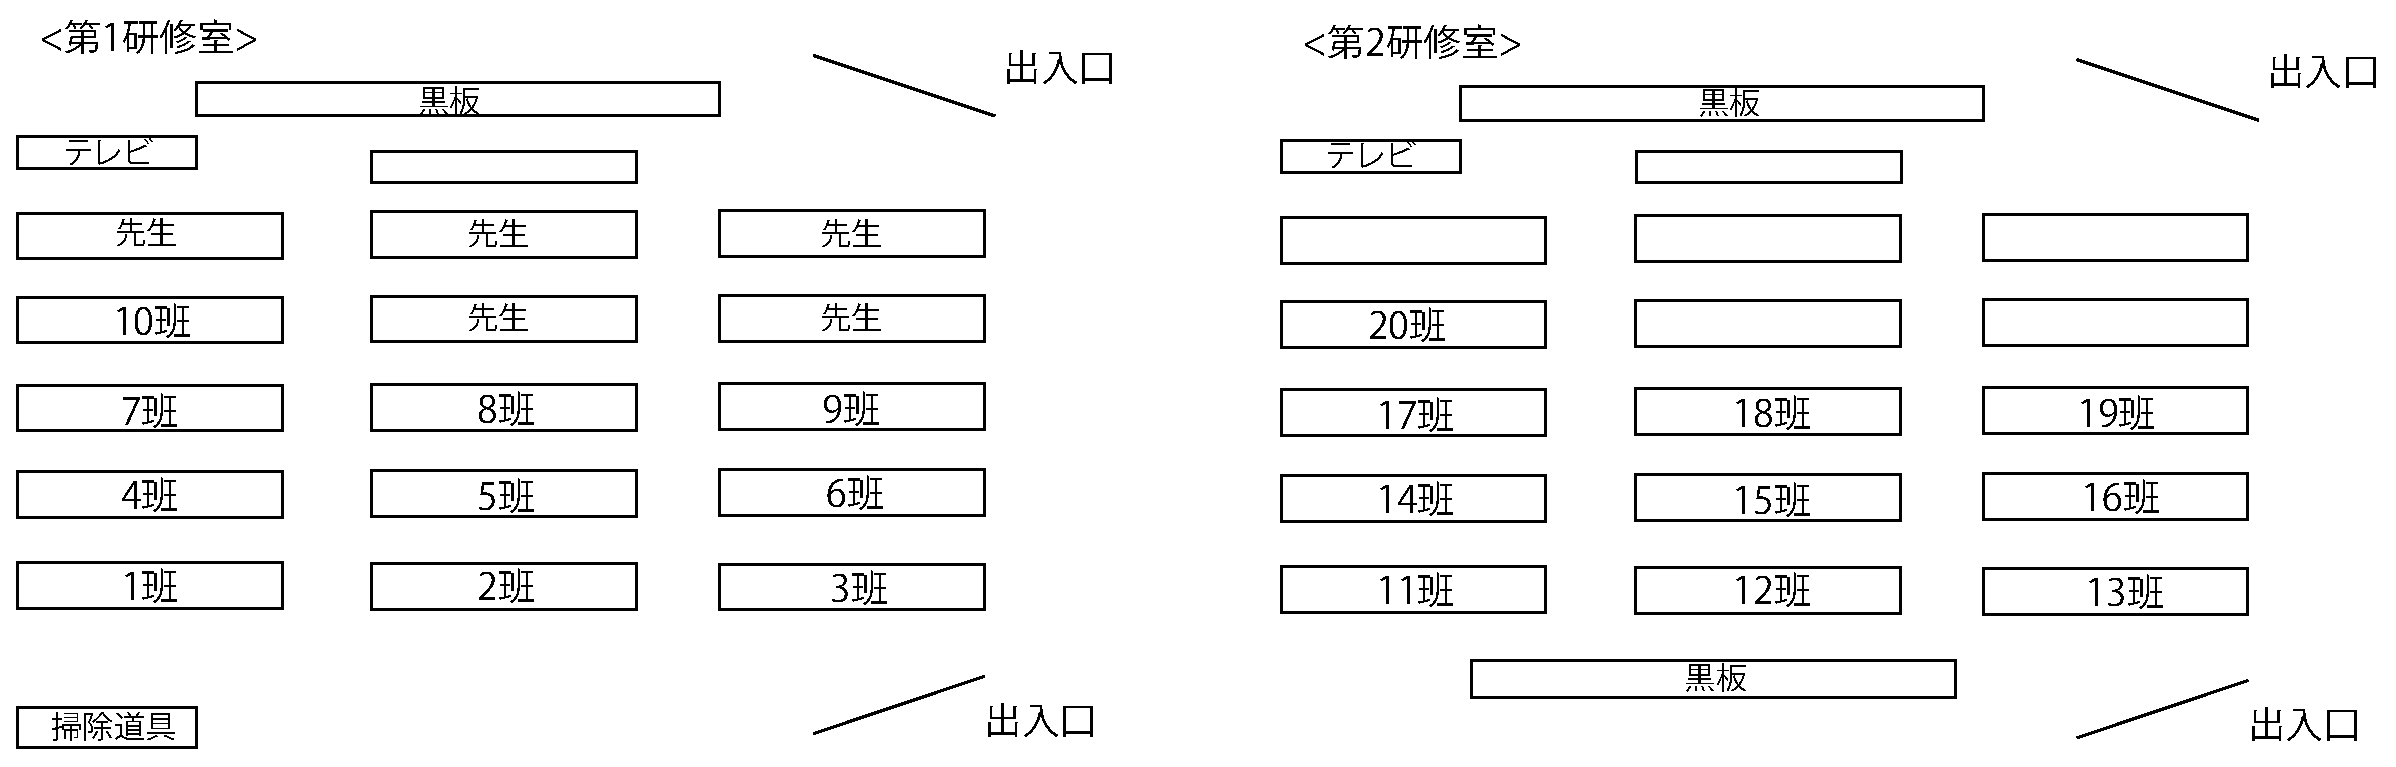
\includegraphics[width=150mm]{./03/nimotsu.eps}
\end{center}
 \caption{第一・二研修室での荷物を置く配置}
 \label{fig:nimotsuhaichi}
\end{figure}
\vspace{-10mm}
\subsubsection{シーツ置き場}

\vspace{-30mm}

\begin{figure}[H]
 \begin{center}
 \hspace{-20mm}
  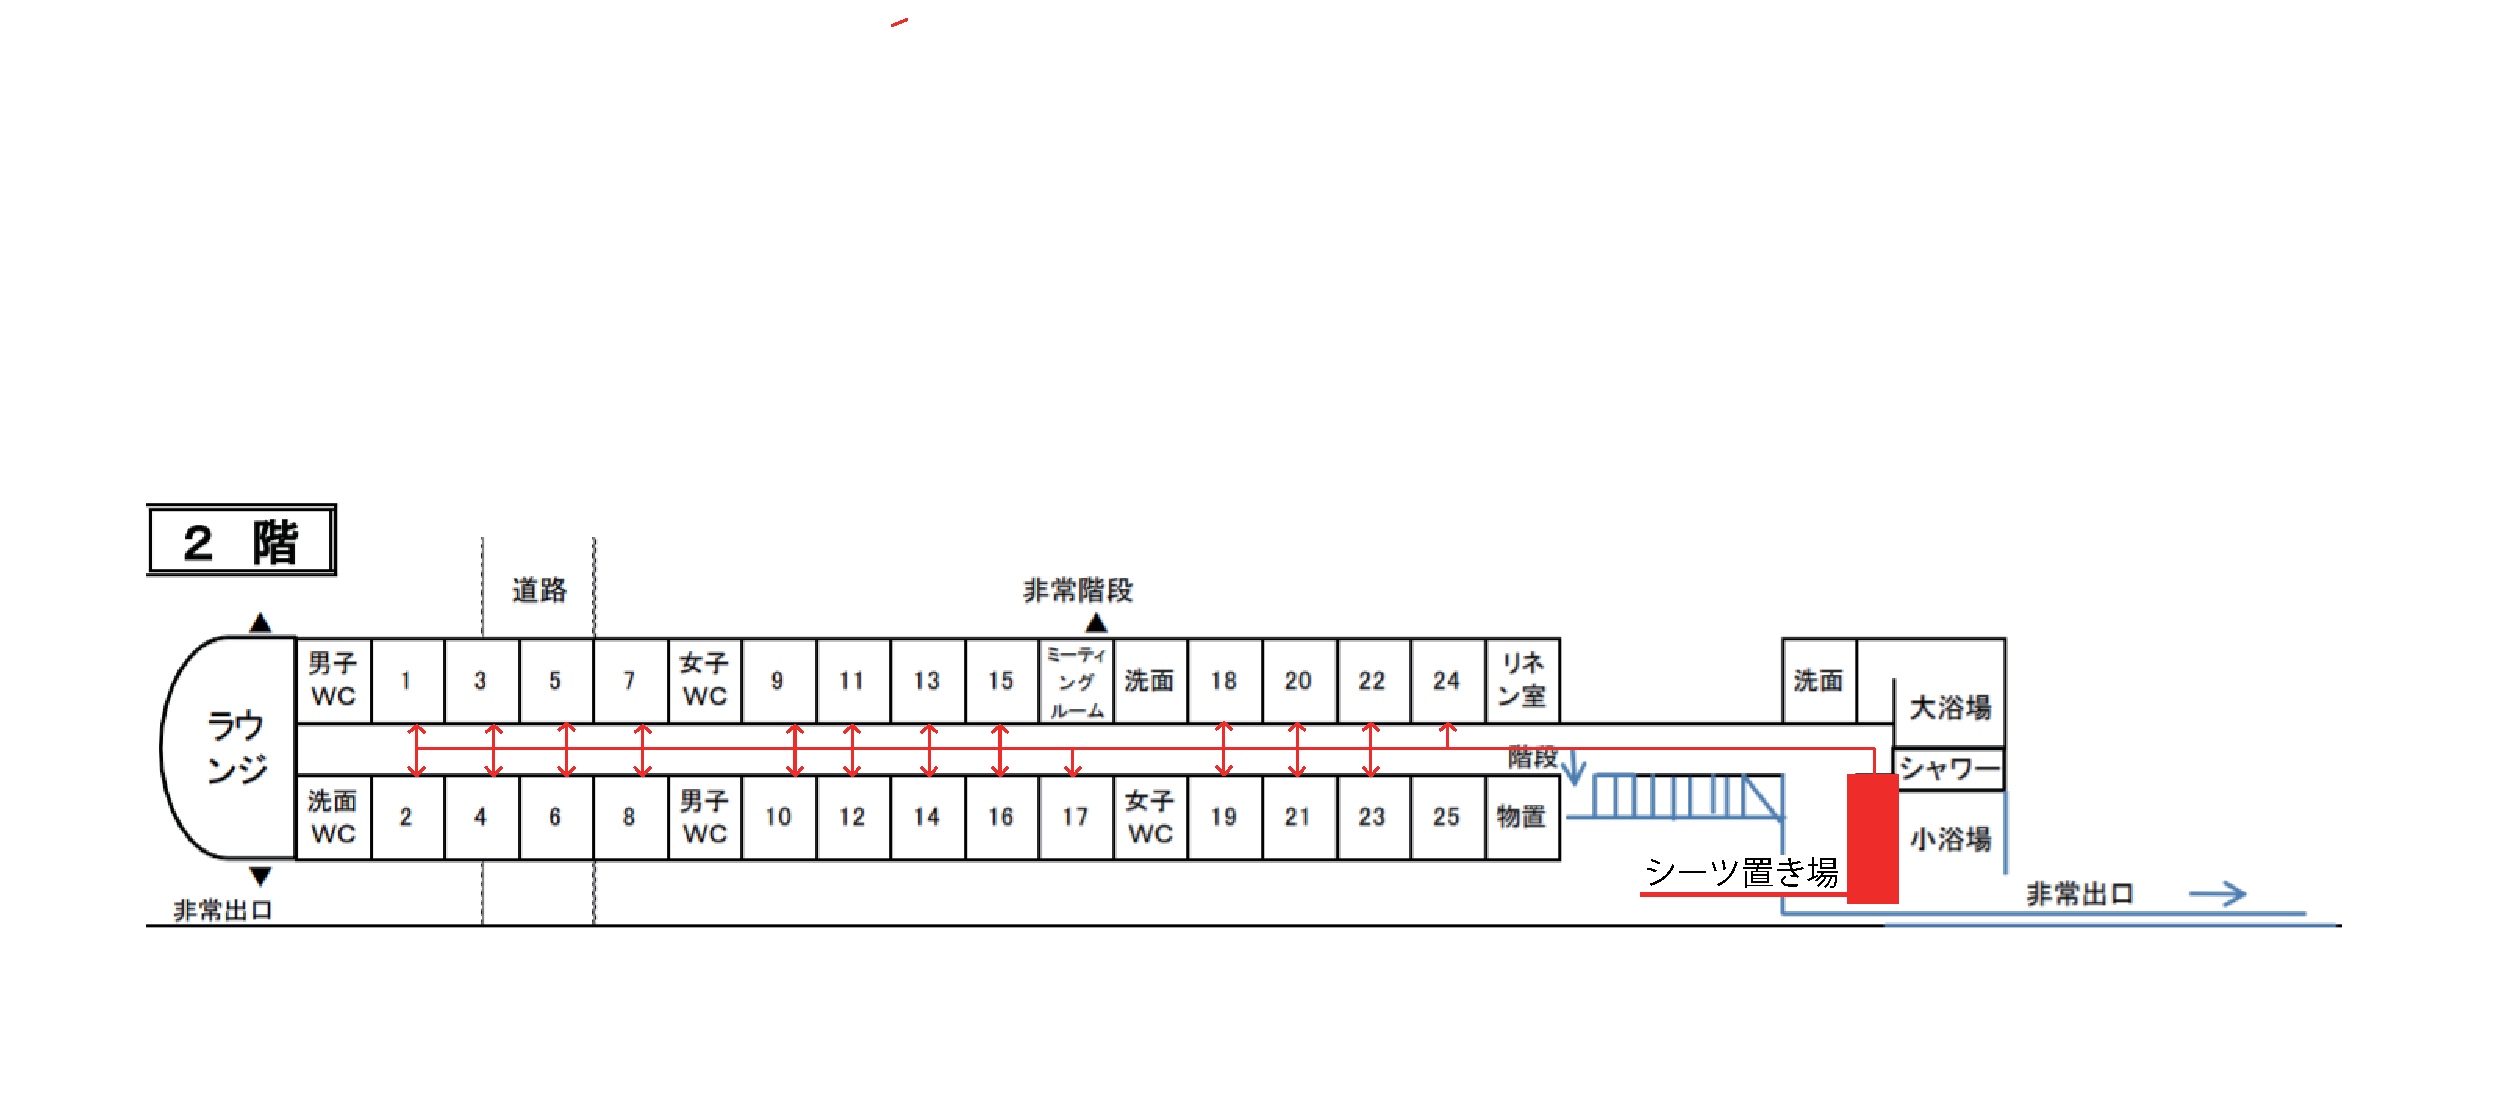
\includegraphics[width=180mm,scale=0.45]{./03/situ.eps}
\end{center}
\vspace{-15mm}
 \caption{シーツを置く位置}
 \label{fig:seatshaichi}
\end{figure}

\subsection{就寝部屋割り}
\begin{figure}[H]
\begin{center}
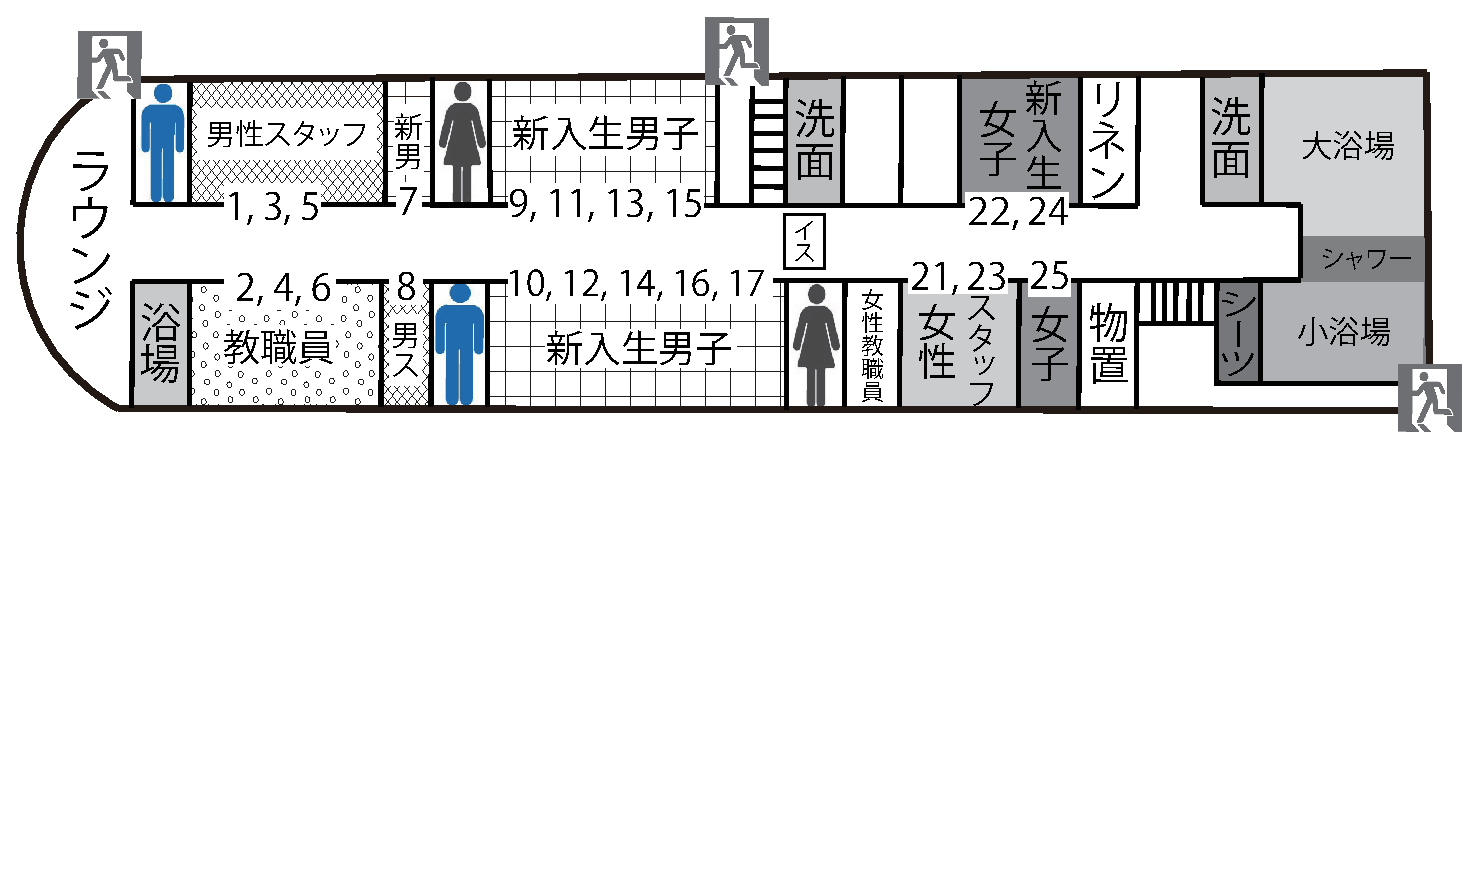
\includegraphics[scale=0.6]{./10/syushin.eps}
\caption{就寝部屋}
\label{fig:shushin}
\end{center}
\end{figure}

\subsubsection{大研修室の配置}
\begin{figure}[H]
 \begin{center}
  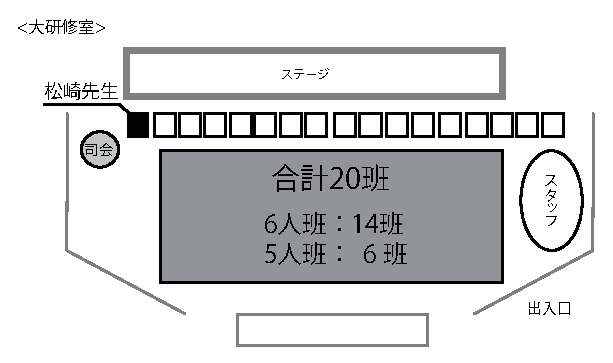
\includegraphics[width=130mm]{./03/nyushoshiki.eps}
  \end{center}
 \caption{大研修室の配置}
 \label{fig:daikenshuhaichi}
\end{figure}

\newpage
\newpage
\subsubsection{大研修室誘導時の配置}
\begin{figure}[htbp]
  \begin{center}
   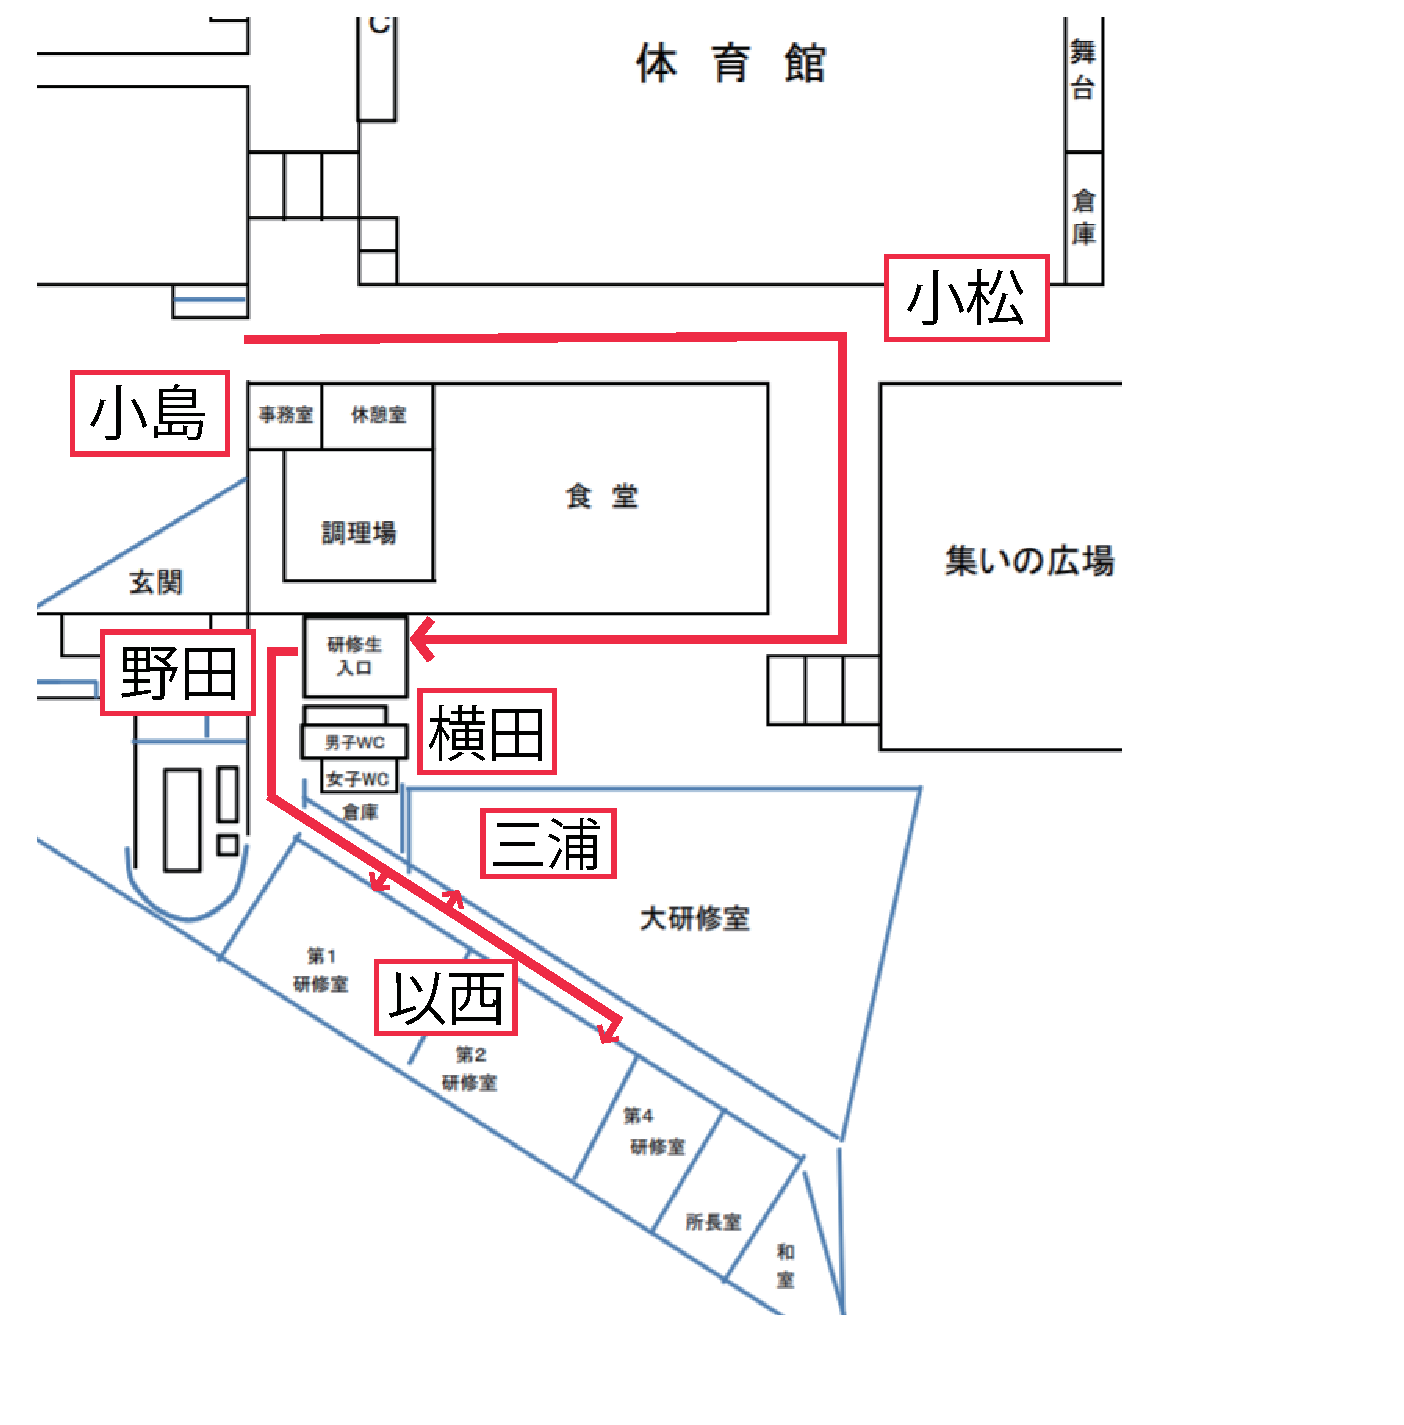
\includegraphics[scale=0.4]{./03/yuudou.eps}
  \end{center}
  \caption{大研修室までの誘導}
  \label{fig:hare}
\end{figure}

%\begin{figure}[htbp]
%  \begin{center}
%   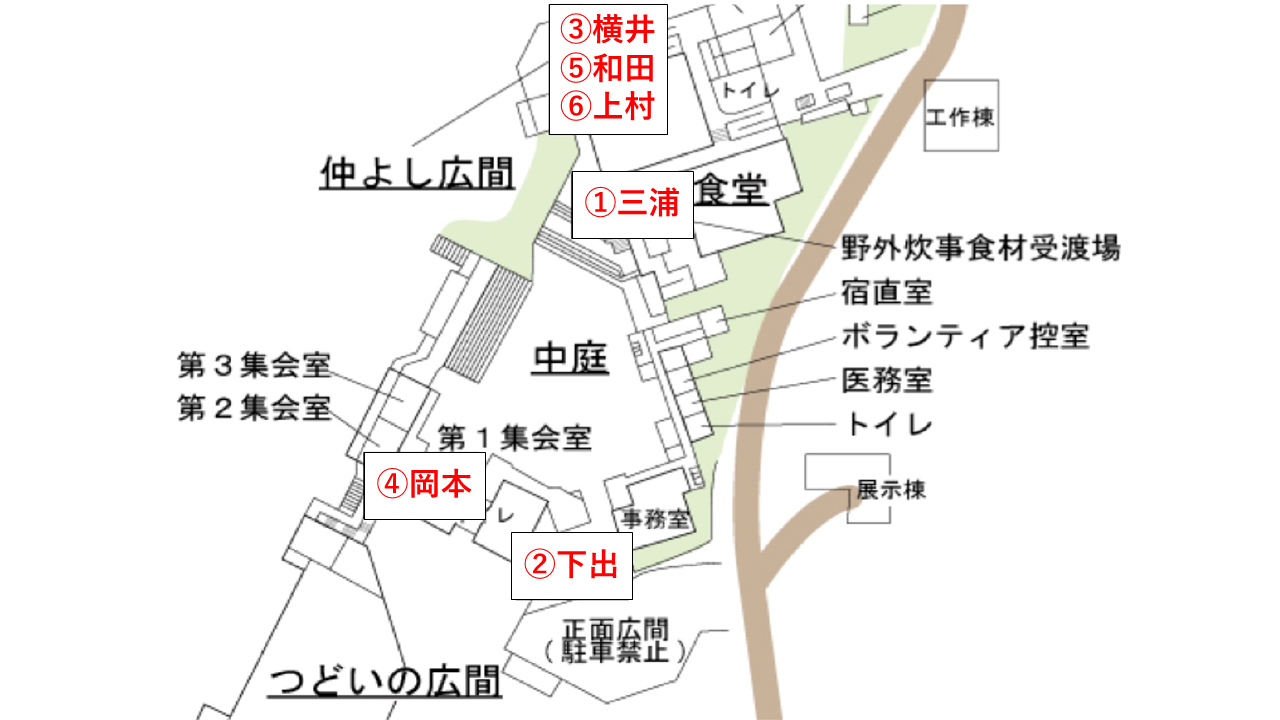
\includegraphics[width=100mm]{./03/yuudou2.eps}
%  \end{center}
%  \caption{大研修室までの誘導 (雨天時)}
%  \label{fig:ame}
%\end{figure}

\subsection{必要物品}
\begin{itemize}
\item 大研修室用の野外炊事班を示したプラカード:20枚
\item 第一・二研修室用の野外炊事班を示したプラカード:20枚
\item 野外炊事場用の野外炊事班を示したプラカード:20枚
\item 教員名を印刷した紙:27枚
\item マスキングテープ(イスに教職員名を貼り付ける用):1つ
\item ブルーシート:1つ
\item プロジェクタ:1つ
\item 野外炊事物品:食器用消毒液(10),ふきん(3枚入り×20),予備の着火剤(5),予備のチャッカマン(2)
\end{itemize}


\subsection{備考}
\begin{itemize}
\item バスの所在を随時連絡してもらうので時間を考えて行動する
\item 先遣隊で連絡を取り合い,終わっていないところの救援を行う
%\item 鍵の又貸しはせず,全ての場合に置いて鍵担当の岡本が鍵管理を行う
\item マイクの電池を確認しておく
\item 入所式に班名が書かれたプラカードを設置する
\item 部屋の鍵は全て開錠(22:00に施錠される)
\end{itemize}


\subsection{連絡事項}
\begin{table}[h]
\begin{tabular}{|c|c|c|c|}
\hline
報告者 & 内容 & タイミング \\ \hline \hline
横田 & 先遣隊 (車2台) 到着 & 到着時\\ \hline
横田 & 準備完了 & 準備完了時 \\ \hline
\end{tabular}
\end{table}

%\include{end}
%%%%%%%%%%%%%%%%%%%%%%%%%%%%%%%%%%%%%%%%%%%%%%%%%%%%%%%%%%%%%%%%%%%%%%%%%%%%%%%

% 必要な項目ができた場合は適宜サブセクションを追加してください
%\include{begin}

% イベント名を記入する
\section{受付(バスに乗るまで)}

% 日時と場所を記入する
% 時刻は4桁で記入すること!
\subsection{日時・場所}

\begin{tabular}{p{2zw}rp{38zw}}
日時 & : & 2019年4月5日(金) 10:15 $\sim$ 12:10\\
場所 & : & 受付用部屋(K101),東ロータリー (バス乗り場)
\end{tabular}


% 目的を記入する
\subsection{タイムスケジュール}
\begin{longtable}{p{3zw}p{39zw}}
10:15 & \textbf{◎ 受付準備開始} \\
      
      & \ \  \underline{受付担当:伊崎,青山,吉田,東} \\
      & \ \  \underline{受付補助担当:高島,日下,小谷,立岩,渡辺,高橋(慎),石野,江川} \\

      & \ \  \ \ \ \textbullet \ \ 学籍番号を示した紙を机の上に貼る\\
      & \ \  \ \ \ \textbullet \ \ 名簿とボールペンを机に並べる\\
      & \ \  \ \ \ \textbullet \ \ 名札を机に並べる\\
      & \ \  \ \ \ \textbullet \ \ 集金ボックスとおつり用のお金を机に置く\\
      & \ \  \ \ \ \textbullet \ \ 準備が終了したら,受付開始まで待機する \\
      & \ \  \ \ \ \textbullet \ \ バス号車の区別が書かれた紙をテーブルに貼る \\\\

      & \ \  \underline{統括担当:藤沢,新川} \\
      & \ \  \ \ \ \textbullet \ \ ホワイトボードにバス号車ごとの新入生の配置を書く(図\ref{fig:uketsuke_k101Haichi}参照) \\
      & \ \  \ \ \ \textbullet \ \ 号車ごとの学籍番号を書く \\
      & \ \  \ \ \ \textbullet \ \ ホワイトボードに以下の諸注意を書く \\\\

      & \ \ 【諸注意】\\
      & \ \  \ \ \ - 学籍番号から各自バスの号車を確認し,受付に移動する(テーブルに号車番号が貼ってある) \\
      & \ \  \ \ \ - バスの乗り込みは12:00から \\
      & \ \  \ \ \ - バスが来るまで荷物は各自で持っておく \\
      & \ \  \ \ \ - 荷物は各自座席に持って行くこと(ただし,大きい荷物(ボストンバック以上)があればバスのトランクに入れる) \\
      & \ \  \ \ \ - 野外炊事,就寝部屋,イベントのグループ,バスの号車は名札に書いている \\
      & \ \  \ \ \ - トイレにいく場合はスタッフに声をかけ,出口(後ろ側)から出る \\
      & \ \  \ \ \ - 必要のある場合以外は教室から出ない \\
      & \ \  \ \ \ - 教室から出るときに忘れ物がないか確認する \\
      & \ \  \ \ \ - 受付を済ませた新入生は名札を身につけ,しおりの9ページにある自己紹介カードを記入する \\
      & \ \  \ \ \ - 食堂でご飯を食べたい新入生はスタッフに声をかけ,11:55までにK101に戻って来る \\\\

      & \ \  \underline{司会担当:塩谷, 中島, 丸田, 高橋(龍), 北村, 藤田(B3)} \\
      & \ \  \ \ \ \textbullet \ \ バス内企画やスケジュールの最終確認を行う\\

      %& \ \  \underline{後遣隊:西森,藤沢} \\
      %& \ \  \ \ \ \textbullet \ \ 自分の荷物を後遣隊の車にのせる \\\\
      %& \ \  \ \ \ \textbullet \ \ 宴の荷物を後遣隊に乗せる \\\\
      
\newpage

11:00 & \textbf{◎ 見回り} \\
      & \ \  \underline{司会:塩谷, 中島, 丸田, 高橋(龍), 北村, 藤田(B3)} \\
      & \ \  \underline{救護車:堀川,貞松} \\
      & \ \  \underline{後遣隊:西森} \\
      & \ \  \underline{見回り担当:角原, 別役,生野,斎藤, 新田} \\
      & \ \  \ \ \ \textbullet \ \ 大学内でK101の位置を知らせる \\\\

11:15 & \textbf{◎ K101への誘導準備} \\
      & \ \  \underline{救護車:堀川,貞松} \\
      & \ \  \underline{後遣隊:西森} \\
      & \ \  \ \ \ \textbullet \ \ K101の入口付近,出口付近,教室内で待機しておく \\\\

11:20 & \textbf{◎ 新入生の受付開始 } \\
      & \ \  \underline{受付担当:伊崎,青山,吉田} \\
      & \ \  \underline{受付補助担当:高島,日下,小谷,渡辺,石野,江川} \\
      & \ \  \ \ \ \textbullet \ \ 新入生が受付にきたら名前を聞いて名簿のチェック欄にチェックをして,参加費(500円)を徴収する \\
      & \ \  \ \ \ \textbullet \ \ 新入生に名札を渡す \\
      & \ \  \ \ \ \textbullet \ \ ホワイトボードに新入生の荷物でトランクに入れる必要があった場合,新入生にタグを渡して名前と野外炊事の班を記入してもらいその荷物にタグをつける \\
      & \ \  \ \ \ \textbullet \ \ その後,各列の席に座らせ,ホワイトボードの諸注意を読んでおくように伝える \\
      & \ \  \ \ \ \textbullet \ \ 大きい荷物の判断は受付担当が行う \\
      & \ \  \ \ \ \textbullet \ \ トイレに行っておくよう連絡する \\
      & \ \  \ \ \ \textbullet \ \ 新入生女子はK101の時点で固まって座るように伝える \\
      & \ \  \ \ \ \textbullet \ \ 女性スタッフは新入生女子に小浴場で入浴できるかどうか確認する \\
      & \ \  \ \ \ \textbullet \ \ 男性スタッフは新入生男子に大浴場で入浴できるかどうか確認する \\
      & \ \  \ \ \ \textbullet \ \ 確認したらチェックリストに書く \\\\

      & \textbf{◎ 先生の受付開始} \\
      & \ \  \underline{受付担当:東} \\
      & \ \  \underline{受付補助担当:立岩,高橋(慎)} \\
      & \ \  \ \ \ \textbullet \ \ 先生は予定時間より早めに来られる可能性があるため注意する \\
      & \ \  \ \ \ \textbullet \ \ 名簿のチェック欄にチェックをしてから名札を渡す \\
      & \ \  \ \ \ \textbullet \ \ 参加費 (2000円)を徴収する \\
      & \ \  \ \ \ \textbullet \ \ 先生の荷物を受け取り,野外炊事の班を記入したタグを付けてK101に置いておく(荷物を見張る) \\
      & \ \  \ \ \ \textbullet \ \ 受付が終了した先生はK101で待機してもらう \\\\

      & \textbf{◎ K101への誘導・アナウンス開始} \\
      & \ \  \underline{統括担当:藤沢,新川} \\
      & \ \  \ \ \ \textbullet \ \ K101の先生方と待機している新入生に対して,適宜,諸注意をアナウンスする \\
      & \ \  \ \ \ \textbullet \ \ トイレには行っておくよう連絡する \\
      & \ \  \ \ \ \textbullet \ \ 受付を済ませた後に食堂に行きたい新入生がいたら,メモを取っていってもらう \\
      & \ \  \ \ \ - このとき11:55までにK101に戻って来るように伝える \\\\

\newpage

      & \ \  \underline{救護車:堀川,貞松} \\
      & \ \  \underline{後遣隊:西森} \\
      & \ \  \ \ \ \textbullet \ \ K101の入口のドアを開ける \\
      & \ \  \ \ \ \textbullet \ \ K101の出口側の通路付近で入口が東側(食堂側)であることを促す \\
      & \ \  \ \ \ \textbullet \ \ K101に入ってきた新入生に対し,各受付がバスの号車ごとに分かれていることを説明しながら誘導する \\
      & \ \  \ \ \ \textbullet \ \ 新入生がトイレにいく場合は出口(グラウンド側)から行かせる \\\\

      & \textbf{◎ バス司会者見回り終了} \\
      & \ \  \underline{司会担当:塩谷, 中島, 丸田, 高橋(龍), 北村, 藤田(B3)} \\
      & \ \  \ \ \ \textbullet \ \ 自分の荷物を持ち,東ロータリーへ移動し,バスが来るのを待つ \\\\

11:40 & \textbf{◎ バス到着} \\
      & \ \  \underline{司会担当:塩谷, 中島, 丸田, 高橋(龍), 北村, 藤田(B3)} \\
      & \ \  \ \ \ \textbullet \ \ バス(運転手:キヨオカ,イノウエ,シモモト)が到着するのでバス司会は待機しておく \\
      & \ \  \ \ \ \textbullet \ \ 担当バスの運転手に挨拶をする \\\\
      
      & \ \  【確認事項】\\
      & \ \  \ \ \ - バス内での飲食の確認 \\
      & \ \  \ \ \ - バス内でのマイクの使用 \\
      & \ \  \ \ \ - その他乗車上の注意 \\
      & \ \  \ \ \ - 自分の荷物をバスのトランクにのせる \\
      & \ \  \ \ \ - 司会担当は,運転手との挨拶後,新入生が来るまでにマイクなどを確認する \\
      & \ \  \ \ \ - 司会担当は,バスの運転手と休憩場所の確認と到着時間の確認をし,確認内容を報告slackに連絡する \\\\

      & \ \  \underline{司会担当1:藤田(B3),中島,丸田} \\
      & \ \  \ \ \ \textbullet \ \ K101に移動し,バスが来たことを受付補助担当に伝える \\\\

      & \ \  \underline{司会担当2:北村,高橋(龍),塩谷} \\
      & \ \  \ \ \ \textbullet \ \ バスのドア付近で待機し,乗車確認の準備をする \\\\


12:00 & \textbf{◎ 新入生の受付終了} \\
      & \ \  \underline{司会担当1:藤田(B3),中島,丸田} \\
      & \ \  \underline{受付補助担当:高島,日下, 小谷, 渡辺,石野,江川} \\
      & \ \  \ \ \ \textbullet \ \ バス到着の連絡がきたら,受付補助担当は自分の荷物を持ち,司会担当と一緒に新入生をバスへ誘導する \\
      & \ \  \ \ \ \textbullet \ \ 混雑を防ぐため,バスの停車順で誘導する \\
      & \ \  \ \ \ \textbullet \ \ 新入生が大きい荷物を持ってきた場合は,バスのトランクに荷物をのせる \\
      & \ \  \ \ \ \textbullet \ \ 受付補助担当は自分の荷物をバスのトランクにのせる \\
      & \ \  \ \ \ \textbullet \ \ 誘導後,司会担当はそのままバスへ,受付補助担当は,K101に戻る \\\\

\newpage

      & \ \  \underline{司会担当2:北村,高橋(龍),塩谷} \\
      & \ \  \ \ \ \textbullet \ \ バスの入口付近で乗車確認リストを用いて,乗車する新入生のチェックを行う \\
      & \ \  \ \ \ \textbullet \ \ 奥からつめて座るように伝える \\
      & \ \  \ \ \ \textbullet \ \ 新入生の女子が1人で来たときは,一旦待機させ,他の女子と隣になるように乗せる \\
      & \ \  \ \ \ \textbullet \ \ バス酔いや体調不良がある人は前方に座らせる \\
      & \ \  \ \ \ \textbullet \ \ 全員が乗車したら,各バスの乗車人数を確認する \\\\

      & \ \  \underline{受付担当:伊崎,吉田,青山} \\
      & \ \  \ \ \ \textbullet \ \ 12:00以降に来た新入生は,受付をした後,K101で待機させておく \\
      & \ \  \ \ \ \textbullet \ \ その際,バス司会に遅れてきた新入生がいることを連絡する \\
      & \ \  \ \ \ \textbullet \ \ 各号車ごとに受付を済ませた新入生の人数をまとめる \\\\

      & \ \  \underline{救護車:堀川,貞松} \\
      & \ \  \ \ \ \textbullet \ \ 自分の荷物を持ち,車を東ロータリーに移動させる \\
      & \ \  \ \ \ \textbullet \ \ 出発の準備をする \\\\

      & \textbf{◎ 先生の受付終了} \\
      & \ \  \underline{受付担当:東} \\
      & \ \  \underline{受付補助担当:立岩,高橋(慎)} \\
      & \ \  \ \ \ \textbullet \ \ 自分の荷物を持つ \\
      & \ \  \ \ \ \textbullet \ \ 新入生の誘導が完了次第,先生をバスに誘導する \\
      & \ \  \ \ \ \textbullet \ \ 全て報告slackを用いて状況を把握し,適宜動く \\\\

12:05 & \textbf{◎ 新入生の乗車確認} \\
      & \ \  \underline{受付担当:伊崎,吉田,青山} \\
      & \ \  \ \ \ \textbullet \ \ 各号車ごとに受付を済ませた新入生の人数をまとめる \\\\

      & \ \  \underline{司会担当:塩谷, 中島, 丸田, 高橋(龍), 北村, 藤田(B3)} \\
      & \ \  \ \ \ \textbullet \ \ 各バスの司会者は,各バスの受付担当と電話で連絡を取り,乗車人数と合うかを確認する \\\\

      & \ \  【乗車人数があわないとき】\\
      & \ \  \ \ \ \textbullet \ \ 受付の名簿にチェックがあるが,バスの乗車確認リストにチェックがない場合 \\
      & \ \  \ \ \ \ \ \ \ \ →補助担当が大学内を探す \\
      & \ \  \ \ \ \textbullet \ \ バスの乗車確認リストにチェックがあるが,受付の名簿にチェックがない場合 \\
      & \ \  \ \ \ \ \ \ \ \ →司会担当がバス内にアナウンスし,その新入生が乗車しているか再確認する \\\\

      & \ \  \underline{受付補助担当:石野,高島,日下,江川,小谷,立岩,高橋(慎)} \\
      & \ \  \underline{見回り担当:角原,渡辺,別役,斎藤,生野,新田} \\
      & \ \  \ \ \ \textbullet \ \ 先生方の荷物を各バスに運ぶ \\
      & \ \  \ \ \ \textbullet \ \ 運んだ後はそのままバスで待機する \\
      & \ \  \ \ \ \textbullet \ \ 荷物が積み終わったら, 吉田が報告slackに連絡する \\
      & \ \  \ \ \ \textbullet \ \ このときK101で待機している新入生がいたら,一緒にバスへ誘導する \\\\
      
      \newpage
      
      & \ \  \underline{受付補助担当:貞松} \\
      & \ \  \ \ \ \textbullet \ \ 貞松は先生受付担当の東から仕事を引き継ぐ \\
      & \ \  \ \ \ \textbullet \ \ 来られた先生の人数をまとめる \\
      & \ \  \ \ \ \textbullet \ \ 先生の受付まわりに忘れ物がないか確認する \\\\

      & \ \  \underline{司会担当:塩谷, 中島, 丸田, 高橋(龍), 北村, 藤田(B3)} \\
      & \ \  \ \ \ \textbullet \ \ バスの入口付近で乗車確認リストを用いて,乗車する先生のチェックを行う \\
      & \ \  \ \ \ \textbullet \ \ 受付担当と連絡を取り,先生の乗車人数があうか確認する \\\\

      & \ \  \underline{後遣隊:西森,藤沢} \\
      & \ \  \ \ \ \textbullet \ \ 藤沢は参加費の計算をする \\
      & \ \  \ \ \ \textbullet \ \ 受付まわりに忘れ物がないか確認する \\
      & \ \  \ \ \ \textbullet \ \ 忘れ物がある場合は司会担当と連絡をとり,
      								忘れ物の特徴などをバス内に伝えてもらうか、早急に対応できそうであれば,
      								忘れ物をバスまで持って行ってもよい \\\\

      & \textbf{◎ 受付完全終了} \\
      & \ \  \underline{受付担当:伊崎,吉田,青山} \\
      & \ \  \ \ \ \textbullet \ \ 全体の受付を終了する \\
      & \ \  \ \ \ \textbullet \ \ 自分の荷物を持ち,バスへ移動する \\
      & \ \  \ \ \ \textbullet \ \ このとき遅れてきた新入生がいた場合は一緒にバスへ誘導する \\
      & \ \  \ \ \ \textbullet \ \ 自分の荷物をバスのトランクにのせ,バスで待機する \\\\
      
      & \ \  \underline{受付担当:貞松} \\
      & \ \  \ \ \ \textbullet \ \ 全体の受付を終了する \\
      & \ \  \ \ \ \textbullet \ \ 救護箱を持っていく \\
      & \ \  \ \ \ \textbullet \ \ 東ロータリーの救護車へ向かう \\\\

      & \ \  \underline{見回り担当:斎藤,角原,別役,新田} \\
      & \ \  \ \ \ \textbullet \ \ 自分の荷物を持ち,バスへ移動する \\
      & \ \  \ \ \ \textbullet \ \ 自分の荷物をバスのトランクにのせ,バスで待機する \\\\

      & \ \  \underline{後遣隊:西森,藤沢} \\
      & \ \  \ \ \ \textbullet \ \ この時間以降の受付は後遣隊が行う \\
      & \ \  \ \ \ \textbullet \ \ 藤沢は参加費を回収する \\
      & \ \  \ \ \ \textbullet \ \ その後,藤沢が物品と参加費を吉田研究室に運ぶ \\\\

12:10 & \textbf{◎ バス・救護車出発} \\
      & \ \  \underline{各スタッフ} \\
      & \ \  \ \ \ \textbullet \ \ バスで移動するスタッフはこの時間までにバスに乗車する \\\\

      & \ \  \underline{救護車:堀川,貞松} \\
      & \ \  \ \ \ \textbullet \ \ 救護車はバスの後ろを追いかける \\\\

\end{longtable}

\newpage

\subsection{人員配置}

\begin{itemize}
\item 受付統括:藤沢,新川
\item 1号車受付:伊崎
\item 1号車受付補助:高島,石野
\item 2号車受付:吉田
\item 2号車受付補助:日下,渡辺
\item 3号車受付:青山
\item 3号車受付補助:小谷,江川
\item 先生受付:東
\item 先生受付補助:立岩,高橋(慎)
\item 1号車司会:北村,藤田(B3)
\item 2号車司会:中島,高橋(龍)
\item 3号車司会:丸田,塩谷
\item 見回り:角原,別役,生野,斎藤,新田
\item 会計:藤沢
\item 救護車:堀川,貞松
\item 後遣隊:西森,藤沢
\end{itemize}

\subsection{バス号車の配置(最終人数により調整)}
\begin{itemize}
\item  1号車:伊崎,斎藤,生野,高島,高橋(慎),石野
\item  2号車:吉田,立岩,日下,渡辺,別役,新田,藤田(M2)
\item  3号車:青山,新川,角原,小谷,東,江川,小野
\end{itemize}

%\clearpage

%\begin{figure}[H]
 % \begin{center}
 %   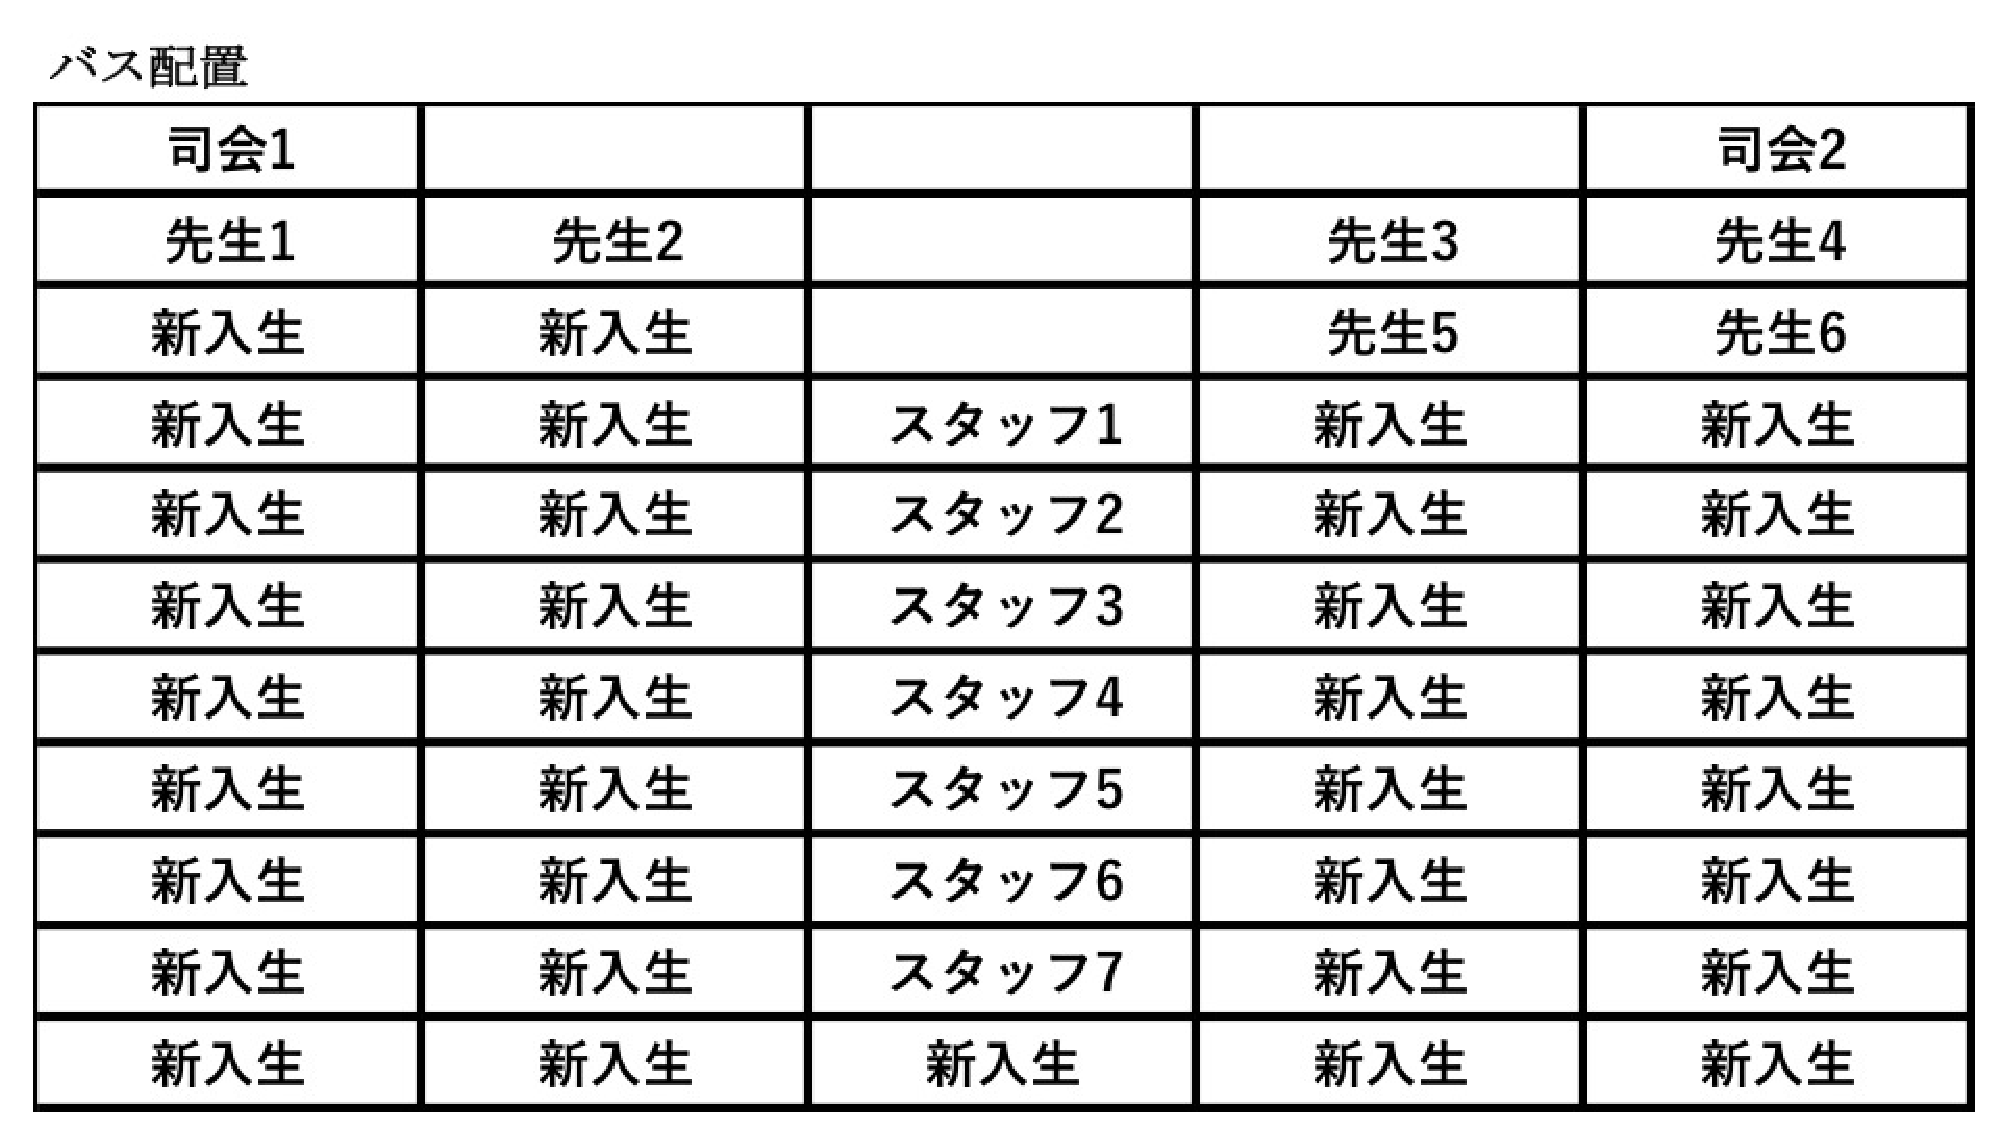
\includegraphics[keepaspectratio, width=15cm]{./04/bus_memberHaichi1.eps}
 %   \caption{バス配置}
 %   \label{fig:bus_memberHaichi1}
%  \end{center}
%\end{figure}

\begin{table}[htb]
  \begin{center}
  \begin{tabular}{|c|c||c||c|c|} \hline
  司会1  & 司会2  &           & 先生1  & 先生2  \\ \hline
  先生3  & 先生4  &           & 先生5  & 先生6  \\ \hline
  新入生 & 新入生 &           & 新入生 & 新入生 \\ \hline
  新入生 & 新入生 & スタッフ1 & 新入生 & 新入生 \\ \hline
  新入生 & 新入生 & スタッフ2 & 新入生 & 新入生 \\ \hline
  新入生 & 新入生 & スタッフ3 & 新入生 & 新入生 \\ \hline
  新入生 & 新入生 & スタッフ7 & 新入生 & 新入生 \\ \hline
  新入生 & 新入生 & スタッフ4 & 新入生 & 新入生 \\ \hline
  新入生 & 新入生 & スタッフ5 & 新入生 & 新入生 \\ \hline
  新入生 & 新入生 & スタッフ6 & 新入生 & 新入生 \\ \hline
  新入生 & 新入生 &  新入生   & 新入生 & 新入生 \\ \hline

  \end{tabular}
\caption{バス内配置}
  \end{center}
\end{table}

\vspace{10mm}

\begin{figure}[H]
  \begin{center}
    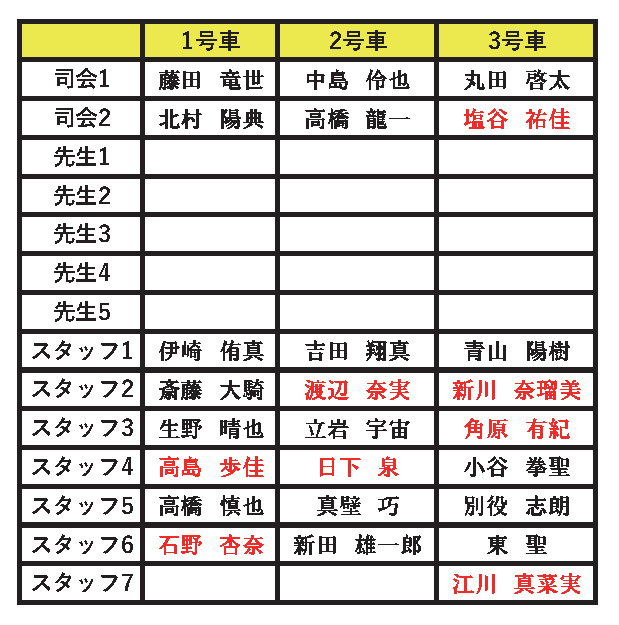
\includegraphics[keepaspectratio, scale=0.9]{./04/bus_memberHaichi2.eps}
    \caption{バス配置}
    \label{fig:bus_memberHaichi2}
  \end{center}
\end{figure}

\subsection{全体配置}
\begin{figure}[H]
  \begin{center}
    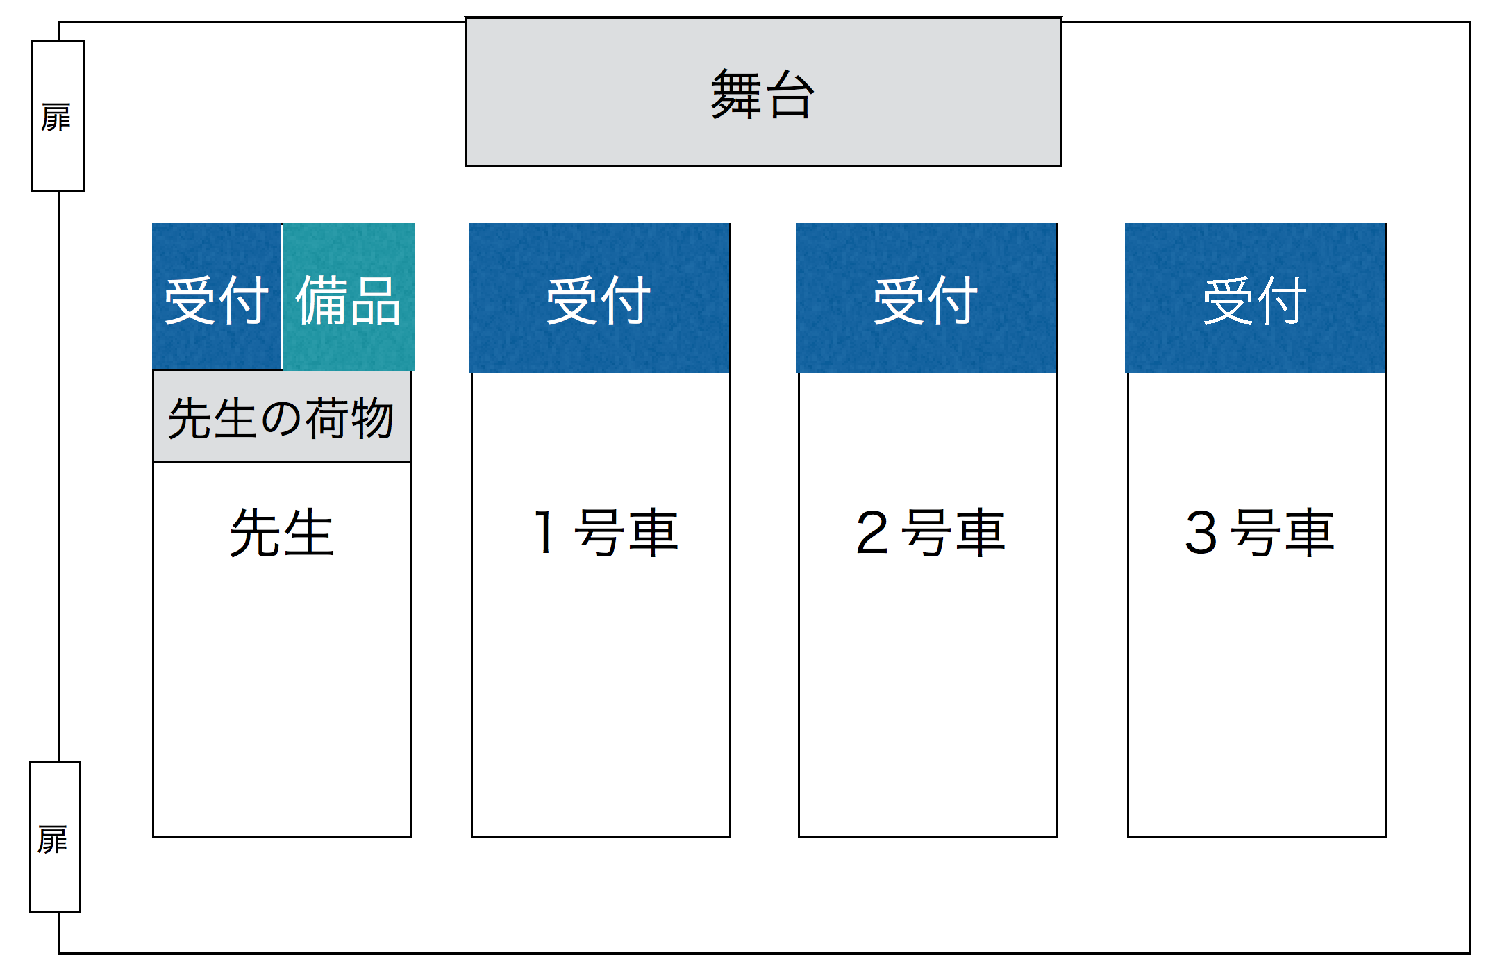
\includegraphics[keepaspectratio, width=14cm]{./04/uketsuke_k101Haichi.eps}
    \caption{K101の全体配置}
    \label{fig:uketsuke_k101Haichi}
  \end{center}
\end{figure}


% イベントに必要な物品と個数を記入する

% 記入例 ・マジックペン 10本


\subsection{必要物品}
\begin{itemize}
\item 名札:人数分
\item 名簿:4部(チェック欄,学籍番号,名前,ふりがなを記載)
\item 名札ケース:人数分
\item しおり:人数分と予備10個
\item 集金ボックス:4箱
\item おつり用のお金:40枚(20000円)
\item ボールペン:4本(受付チェック用)
\item ホッチキス:5個(荷物のタグ付け用)
\item 紙:4枚(学籍番号を示した紙3枚,先生用1枚)
\item マスキングテープ:1個(紙を貼るとき用)
\item 荷物用のタグ:人数分(先生・荷物を預けた新入生・スタッフ用)
\item 乗車確認リスト:3部(バスの乗車確認用)
\item 予備のしおり:10部
\end{itemize}

\newpage

\subsection{備考}
\begin{itemize}
\item K101は7:00から使用できる
\item K101:258席,座席は前から詰めて座るようにする
\item バスのトランクには原則新入生の荷物はのせない ただし,キャリーバッグなど大きい荷物はのせてもよい
\item スタッフの荷物はバスのトランクにのせる ただし,先遣隊・救護車・後遣隊は各自で持っていく 当日集まったとき,スタッフは自分の荷物にタグをつける
\item 会計担当は当日までにおつり用のお金を用意しておく
\item 受付担当はホッチキスとボールペンを用意しておく
\item 受付は速やかに行動する
\item 新入生と関わる一番はじめの場なので明るく元気な挨拶を心がける
\item 新入生のオリエンテーション時に荷物を置ける余裕がないことを知らせておく
\item 人員配置されていないスタッフは,基本的に見回りにまわる
\item バス内連絡(高島,吉田,江川)は一番前のスタッフ席に座る 
\end{itemize}



% \subsection{連絡事項}
% \begin{table}[h]
% \begin{tabular}{|c|c|c|c|c|} \hline
% 報告者                 & 対象   & 内容                           & タイミング             & 備考   \\ \hline
% 川添                   & 全体   & バスが到着したこと             & バス到着時             &        \\ \hline
% 各バス司会             & 各受付 & 各号車の新入生の乗車人数確認   & 新入生乗車後           & 電話で \\ \hline
% 各バス司会             & 全体   & 新入生の乗車人数を確認したこと & 新入生の乗車人数確認後 &        \\ \hline
% 河野,下出,植田       & 全体   & 新入生の遅刻者の有無           & 新入生の乗車人数確認後 &        \\ \hline
% 各バス司会             & 各受付 & 各号車の先生の乗車人数確認     & 先生乗車後             & 電話で \\ \hline
% 各バス司会             & 全体   & 先生の乗車人数を確認したこと   & 先生の乗車人数確認後   &        \\ \hline
% 領内                   & 全体   & 先生の遅刻者の有無             & 先生の乗車人数確認後   &        \\ \hline
% 司会補助               & 全体   & 先生の荷物の積み込み完了       & 荷物も積み込み完了後   &        \\ \hline
% 手塚,川添,本田,鈴木(夏) & 全体 & 各バス,救護車が出発したこと & バス,救護車出発時     &        \\ \hline
% \end{tabular}
% \end{table}

%\include{end}

%\include{begin}

\section{後遣隊}

\subsection{日時・場所}

\begin{tabular}{p{2zw}rp{38zw}}
  日時 & : & 2019年4月5日(金) 12:30 $\sim$ 15:00\\
  場所 & : & ????, ????,車内
\end{tabular}

\subsection{タイムスケジュール}
% 時刻は必ず4桁(00:00)で書くこと!!!


\begin{longtable}{p{3zw}p{39zw}}
  12:30 & \textbf{◎ 片付け} \\
        & \ \ \textbullet \ \ ????, ????の片付けをする \\
        & \ \ \textbullet \ \ その後,忘れ物の確認をする \\
        & \ \ \textbullet \ \ 会計係藤沢は参加費を(?任)研究室に持って行き,保管しておく\\\\

  12:50 & \textbf{◎ 出発準備} \\
        & \ \ \textbullet \ \ 忘れ物を車に運ぶ \\
        & \ \ \textbullet \ \ この時間までに遅刻者の対応を終わらせる\\
        & \ \ \textbullet \ \ 忘れ物がないか最終確認をする\\
        & \ \ \textbullet \ \ ????, ????を退出するとき,電気の消灯などの確認をする\\\\

  13:00 & \textbf{◎ 出発} \\
        & \ \ \textbullet \ \ 西森車は途中で飲み物を冷やすための氷を買う \\
        & \ \ \textbullet \ \ 先遣隊がリストアップした不足物がある場合は購入する \\\\

  15:00 & \textbf{◎ 幡多到着} \\
        & \ \ \textbullet \ \ 遅刻者がいない場合\\
        & \ \ \ \ \ - 幡多到着後,自分の荷物を?第一集会室に置く\\
        & \ \ \ \ \ - その後,本隊と合流する\\
        & \ \ \textbullet \ \ 遅刻者がいる場合\\
        & \ \ \ \ \ - 幡多青少年の家付近になったら,鍵係(?岡本)と連絡をとる\\
        & \ \ \ \ \ - 到着後,鍵係(?岡本)に荷物置きの部屋を開けてもらい,遅刻した新入生の荷物と自分の荷物を置く\\
        & \ \ \ \ \ - 遅刻した新入生を連れて本隊と合流する\\
\end{longtable}


\subsection{人員配置}
\begin{itemize}
\item 後遣隊(西森車):西森,藤沢
\subsection{必要物品}
\begin{itemize}
  \item 夜の荷物(おつまみ,皿,紙コップ,キッチンペーパー,新入生用のお菓子,飲み物,懐中電灯4本)
\end{itemize}
\end{itemize}

%\include{end}


%%\include{Begin}

\section{バス内(行き)}

\begin{tabular}{p{2zw}rp{38zw}}
  日時 & : & 2019年4月5日(金) 12:10 $\sim$ 14:40\\ %未定
  場所 & : & バス
\end{tabular}

\subsection{目的}
新入生の緊張をほぐし,仲を深める.


\subsection{タイムスケジュール}
% 時刻は必ず4桁(00:00)で書くこと!!!
\begin{longtable}{p{3zw}p{39zw}}
  12:10 & \textbf{◎ バス出発 } \\
        & \ \ \textbullet \ \ 連絡係(伊崎,吉田,江川)は受付との乗車チェックが終わり次第,乗車チェックが完了したことを報告slackに連絡する \\
        & \ \ \textbullet \ \ 全車の乗車チェックが終わり次第,出発する \\
        & \ \ \textbullet \ \ 連絡係はバスが出発したことを報告slackに連絡する \\
	    & \ \ \textbullet \ \ 連絡係はバスの状況を見て話し始める \\\\

        & \textbf{◎ 司会者挨拶,自己紹介} \\     
        & \textbf{◎これからの流れ説明 } \\
        & \textbf{◎ バス内諸注意,スタッフ紹介} \\   
        & \textbf{◎ 流れ説明} \vspace{5mm} \\
        
  12:35 & \textbf{◎ 道の駅(風良里)到着} \\
	    & \ \  \textbullet \ \ 補助席に座ってる人が先に降りる \\
	    & \ \  \textbullet \ \ スタッフは新入生の奇行に目を配る \\
	    & \ \  \textbullet \ \ バス連絡係は報告slackで到着の旨を連絡する \\\\

  12:45 & \textbf{◎ 乗車開始} \\
  	    & \ \  \textbullet \ \ 気分が悪い人がいないか確認する(もしいた場合は救護車に移動してもらう) \\
	    & \ \  \textbullet \ \ 司会者は新入生に隣の席の人がいるか確認してもらい,人数を確認する \\
	    & \ \  \textbullet \ \ バス連絡係はバス司会は報告slackで乗車開始の旨を連絡する \\\\
	
  12:50 & \textbf{◎ 道の駅(風良里)出発} \\
	    & \ \  \textbullet \ \ 運転手に乗車確認を伝え順次出発する\\
	    & \ \  \textbullet \ \ バス連絡係は報告slackで出発の旨を連絡する\\\\

        & \textbf{◎ 教員紹介} \\ 
        & \textbf{◎ バス内企画 その1} \\
      	& \ \  \textbullet \ \ 自己紹介ゲーム \\
        & \textbf{◎ バス内企画 その2} \\
		& \ \  \textbullet \ \ 方言当てゲーム \vspace{5mm} \\
        
  13:50 & \textbf{◎ あぐり窪川到着} \\
	    & \ \  \textbullet \ \ 補助席に座ってる人が先に降りる \\
	    & \ \  \textbullet \ \ スタッフは新入生の奇行に目を配る \\
	    & \ \  \textbullet \ \ バス連絡係は報告slackで到着の旨を連絡する \\\\

  14:15 & \textbf{◎ 乗車開始} \\
	    & \ \  \textbullet \ \ 気分が悪い人がいないか確認する(もしいた場合は救護車に移動してもらう) \\
	    & \ \  \textbullet \ \ 司会者は新入生に隣の席の人がいるか確認してもらい,人数を確認する \\
	    & \ \  \textbullet \ \ バス連絡係は報告slackで乗車開始の旨を連絡する \\\\

  14:20 & \textbf{◎ あぐり窪川出発} \\
	    & \ \  \textbullet \ \ 運転手に乗車確認を伝え順次出発する \\
	    & \ \  \textbullet \ \ バス連絡係は報告slackで出発の旨を連絡する \\\\

        & \textbf{◎ バス内企画 その3} \\
	    & \ \  \textbullet \ \ 100分の1ゲーム \vspace{5mm} \\
  
  15:05 & \textbf{◎ 幡多到着5分前} \\
	    %& \ \  \textbullet \ \ タイムライン上は到着5分前だが本番は山道に入ったところでもうすぐ着くというアナウンスをする \\
        & \ \  \textbullet \ \ 名札をつけていることを確認してもらい,野外炊事のグループを名札で確認をしてもらう \\
        & \ \  \textbullet \ \ トイレ,荷物について説明する \\
        & \ \  \textbullet \ \ 入所式の並び方を説明する \\
	    & \ \  \textbullet \ \ バス連絡係は報告slackで山道に入った旨を連絡する \\\\

  15:10 & \textbf{◎ 幡多到着} \\
        & \ \ \textbullet \ \ 到着後スタッフは速やかに降りて荷下ろしをする \\
	    & \ \ \textbullet \ \ 3号車は2号車の荷下ろしの手伝いをする \\
	    & \ \ \textbullet \ \ 道の駅(風良里)とあぐり窪川の休憩とは違い全員がバスから降りるので前から順に速やかに降りてもらう \\
        & \ \ \textbullet \ \ 到着した旨を報告slackに連絡する \\\\
\end{longtable}

%%\subsection{内容}
\subsection{人員配置(表5,図\ref{fig:bus_memberHaichi2},参照)}
○1号車
\begin{itemize}
\item 司会:藤田,北村
\item 補助: 伊崎,斎藤,生野,高島,高橋(慎),石野
\end{itemize}
○2号車
\begin{itemize}
\item 司会:中島,高橋(龍)
\item 補助: 吉田,渡辺,立岩,日下,新田,別役

\end{itemize}
○3号車
\begin{itemize}
\item 司会:丸田,塩谷
\item 補助: 青山,新川,角原,小谷,東,江川

\end{itemize}


\subsection{トランク内荷物配置図}
\begin{figure}[H]
\begin{tabular}{lr}
\begin{minipage}{1.0\textwidth}
  \begin{center}
  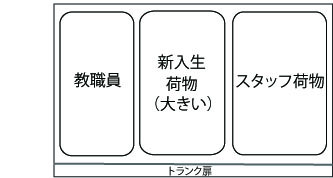
\includegraphics[width=8cm]{./06/baggage_place_1.eps}
  \caption{トランク内荷物配置図(1,2,3号車)}
  \end{center}
\end{minipage}
\end{tabular}
\end{figure}

\subsection{必要物品}
\begin{itemize}
\item 酔い止め薬:各バス1箱
\item エチケット袋:各バス2枚
\item 紙コップ:各バス5個
\item 水(常温):各バス500ml(1本)
\item 100分の1ゲームの商品:野外炊事に使用する調味料3種類*3セット
\end{itemize}

\subsection{備考}

\begin{itemize}
\item 連絡係が報告slackに連絡を入れる
\item 先遣隊,他のバス,後遣隊等と随時連絡を取り合う
\item 新入生の体調確認を忘れない
\end{itemize}


%%\include{End}

% 必要な項目ができた場合は適宜サブセクションを追加してください
%\include{begin}

% イベント名を記入する
\section{幡多到着}

% 日時と場所を記入する
% 時刻は4桁で記入すること!
\subsection{日時・場所}
\begin{tabular}{p{2zw}rp{38zw}}
  日時 & : & 2019年4月5日(金) 14:40 $\sim$ 15:00\\
  場所 & : & バス内 〜 大研修室 
\end{tabular}

% イベントのタイムスケジュールを記入する
% 時刻は必ず4桁(00:00)で記入すること!
% 時間の流れは途切れないように記述する!
\subsection{タイムスケジュール(晴天)}
\begin{longtable}{p{3zw}p{39zw}}
  15:00 & \textbf{◎ バス到着・案内} \\
        & \ \   \textbullet \ \ 先遣隊(以西)ほかの者は降車場所〜大研修室の道中に誘導員として配置し,新入生の誘導をバス司会スタッフとともに行う(配置場所は図\ref{fig:hare}参照)\\
        & \ \   \textbullet \ \ 上記以外の先遣隊は大研修室に向かう \\
        & \ \   \textbullet \ \ 本隊はバス到着後乗っている新入生の荷物を降ろす\\
        & \ \   \textbullet \ \ 1号車荷卸スタッフ(伊崎,斎藤,高橋(慎))と2号車荷卸スタッフ(吉田,立岩,真壁)と3号車荷卸スタッフ(小谷,青山,東)はそれぞれ1号車,2号車,3号車の荷卸をする\\
        & \ \   \textbullet \ \ 荷卸の優先順位は高い順からスタッフ→教職員→新入生となる(尚,教職員の荷物はなるべく手渡しとする)\\
        & \ \   \textbullet \ \ 1号車の荷卸スタッフ(伊崎,斎藤,高橋(慎))は1号車の荷卸が高橋(慎)で行えると判断した場合,伊崎,斎藤は速やかに自分の荷物を持ち第一・二研修室に運ぶ \\
        & \ \   \textbullet \ \ 2号車の荷卸スタッフ(吉田,立岩,真壁)は2号車の荷卸が真壁で行えると判断した場合,吉田,立岩は速やかに自分の荷物を持ち第一・二研修室に運ぶ \\
        & \ \   \textbullet \ \ 3号車の荷卸スタッフ(小谷,  青山,東)は3号車の荷卸が東で行えると判断した場合,小谷,別役は速やかに自分の荷物を持ち第一・二研修室に運ぶ \\
        & \ \   \textbullet \ \ ワゴン車の荷卸スタッフ(別役,生野)はワゴン車の荷物を第一・二研修室に移動する \\
        & \ \   \textbullet \ \ バスから降りたスタッフは速やかに自分の荷物を第一・二研修室に運ぶ \\
        & \ \   \textbullet \ \ 新入生は1号車,2号車,3号車の順番で降車させる \\
        & \ \   \textbullet \ \ 荷卸などで持って行くことができないスタッフは各バスの司会に運んでもらう \\
        & \ \   \textbullet \ \ 第一・二研修室配置のスタッフ(以西)は新入生・教職員の荷物を班ごとにまとめて置かせ,大研修室に行くように誘導する(その際しおりは持って行くようにさせる) \\
        & \ \   \textbullet \ \ トイレに行きたい新入生がいる場合,横田はトイレの場所を伝え、行くように促す \\
        & \ \   \textbullet \ \ 各班代表スタッフは迅速に大研修室へ移動する \\
        & \ \   \textbullet \ \ 各班代表スタッフは班名の書かれたプラカードを持ち,教職員と対面させるように新入生の整列を行う \\
        & \ \   \textbullet \ \ 整列後,新入生を出入り口側に向かせて座らせ,スタッフはステージ向かって右側に移動する \\
        & \ \   \textbullet \ \ 各班代表スタッフは班員が揃い次第司会に報告する \\
        & \ \   \textbullet \ \ 立岩(司会)はどの班が揃っているか適宜確認を行う \\ 
        & \ \   \textbullet \ \ 後遣隊の荷物が第一・二研修室に置かれたら,鍵係は第一・二研修室を施錠する \\\\

  15:15 & \textbf{◎ 各班整列完了・教員誘導完了} \\
        & \ \   \textbullet \ \ 各班代表者は大研修室に入ってきた新入生を班ごとに誘導する \\
        & \ \   \textbullet \ \ 出席する新入生・教職員が揃い次第,入所式を開始 \\
        & \ \   \textbullet \ \ 施設職員呼び出し係(東)は、準備が完了しそうになったら施設職員さんを呼びに行く \\
\end{longtable}

\subsection{タイムスケジュール(雨天)}
\begin{longtable}{p{3zw}p{39zw}}
  15:00 & \textbf{◎ バス到着・案内} \\
        & \ \   \textbullet \ \ 先遣隊(以西)は降車場所〜大研修室の道中に誘導員として配置し,新入生の誘導を行う(配置場所は図\ref{fig:hare}参照) \\
        & \ \   \textbullet \ \ 上記以外の先遣隊は大研修室に向かう \\
        & \ \   \textbullet \ \ 本隊はバス到着後スタッフ全員でトランクの荷物を玄関に降ろす.(この時,各バスに乗っている新入生と教職員はバス内で待機する) \\
        & \ \   \textbullet \ \ 1号車・2号車・3号車の司会スタッフは荷物を運び終えたらバスで待機している新入生と教職員を誘導しに行く \\
        & \ \   \textbullet \ \ ワゴン車の荷卸スタッフ(生野,別役)はワゴン車の荷物を第一・二研修室に移動する \\
        & \ \   \textbullet \ \ 1号車・2号車・3号車の荷卸スタッフは終わった時点でワゴン車の荷卸を手伝い,全ての荷卸が終了次第大研修室に移動する \\
        & \ \   \textbullet \ \ 第一・二研修室配置のスタッフ(以西)は新入生・教職員の荷物を班ごとにまとめて置かせ,大研修室に行くように誘導する(その際しおりと傘は持って行くようにさせる)\\
        & \ \   \textbullet \ \ トイレに行きたい新入生がいる場合,以西はトイレの場所を伝え、行くように促す \\
        & \ \   \textbullet \ \ 袋配布スタッフ (藤田,日下) はなかよし広間入り口前で傘入れ袋を配布する \\
     & \ \   \textbullet \ \ 研修生入り口で折り畳み傘は傘入れ用のビニール袋に入れてもらい,長い傘は傘立てか壁に立てかける \\
        & \ \   \textbullet \ \ 各班代表スタッフは迅速に大研修室へ移動する \\
        & \ \   \textbullet \ \ 各班代表スタッフは班名の書かれたプラカードを持ち,教職員と対面させるように新入生の整列を行う \\
        & \ \   \textbullet \ \ 整列後,新入生を出入り口側に向かせて座らせ,スタッフは柱の後ろに移動する \\
        & \ \   \textbullet \ \ 立岩(司会)はどの班が揃っているか適宜確認を行う \\\\

  15:15 & \textbf{◎ 各班整列完了・教員誘導完了} \\
        & \ \   \textbullet \ \ 各班代表者は大研修室に入ってきた新入生を班ごとに誘導する \\
        & \ \   \textbullet \ \ 新入生を座らせ司会者へ報告する \\
        & \ \   \textbullet \ \ 出席する新入生・教職員が揃い次第,入所式を開始 \\
        & \ \   \textbullet \ \ 準備が終わりそうになったら,施設職員呼び出し係(東)が幡多職員さんを呼びに行く \\
\end{longtable}


% イベントに必要な役割と人数を記入する
% 担当者は決定次第追記する
% 記入例 ・司会者 2人(名前1、名前2)
\subsection{人員配置(人数により調整あり)}
\begin{itemize}

\item 1号車荷卸スタッフ:伊崎,斎藤,高橋(慎)
%山口 三浦 早瀬
\item 2号車荷卸スタッフ:吉田,立岩,真壁

\item 3号車荷卸スタッフ:小谷,青山,東
%横井 西井 森
\item ワゴン:生野,別役

\item 誘導係:北村,中島,高橋,丸田,塩谷,藤田
%川添 東 藤田
\item 袋配布:藤田,日下

\item 施設職員呼び出し係:東
  %島田
\item 司会:立岩
\end{itemize}


% イベントに必要な物品と個数を記入する
% 記入例 ・マジックペン 10本
\subsection{必要物品}
\begin{itemize}
%\item 靴を入れる袋:200枚
\item 傘を入れる袋:200枚
\end{itemize}


% 注意事項やスタッフに周知しておくべきことがあれば記入する
\subsection{備考}
\begin{itemize}
\item 大研修室での整列は,野外炊事の班で固まって集まるようにし,集まったことが確認できたらその場で座りやすいように列をある程度崩してもよい
\item トランクに荷物を入れている荷卸スタッフの荷物は各バス司会が運び第一・二研修室まで運ぶ
\item タグに野外炊事班を書いておく
\item 晴天時と雨天時でタイムスケジュールが多少異なるので注意する
\item ワゴンの荷物は第一・二研修室に運ぶ
\end{itemize}


%\include{end}

% 必要な項目ができた場合は適宜サブセクションを追加してください

%\include{begin}

\section{入所式・教員紹介}

\subsection{日時・場所}
\begin{tabular}{p{2zw}rp{38zw}}
  日時 & : & 2019年4月5日(金) 15:30$\sim$16:10\\
  場所 & : & 大研修室
\end{tabular}

\subsection{目的}
施設の円滑な利用と利用規約について理解を促す.また,新入生に今後お世話になる教職員の方々を覚えてもらうきっかけを作る.

\subsection{タイムスケジュール}
\begin{longtable}{p{3zw}p{39zw}}
  15:30 & \textbf{◎ 入所式開始} \\
  %小野
        & \ \ \textbullet \ \ 司会者(立岩)の簡単な挨拶と,代表(宮尾)の紹介をする\\
        & \ \ \textbullet \ \ 代表による施設職員と新入生に向けた挨拶をする\\\\

  15:35 & \textbf{◎ 教員紹介開始} \\
        & \ \ \textbullet \ \ 司会者は新入生を教員と対面させ,教員紹介の説明をする \\
        & \ \ \textbullet \ \ 司会者は教職員にマイクをリレー形式で渡していただくよう伝える \\
        & \ \ \textbullet \ \ 司会者は最初の教職員にマイクを渡し,並んでいる新入生の後ろ側を通り,スタッフの待機場所に移動する  \\
        & \ \ \textbullet \ \ 司会者は最後の教職員の近くで待機する \\
        & \ \ \textbullet \ \ 教職員に自己紹介を行ってもらう(1分/人) \\
        & \ \ \textbullet \ \ 教職員の自己紹介が終わり次第,司会者は最後の教職員からマイクをもらう\\
        & \ \ \textbullet \ \ 司会は教員紹介に参加できない先生と遅刻する先生の紹介を始める\\\\

  16:00 & \textbf{◎ 教員紹介終了} \\ %教員紹介が押すと推定
        & \ \ \textbullet \ \ 司会者は各スタッフを野外炊事の担当の班の出口側に並ぶように伝える \\
        & \ \ \textbullet \ \ この時待機していたスタッフは担当の班の先頭に並ぶ\\
        & \ \ \textbullet \ \ 司会者はスタッフに座るよう指示する\\\\

  16:05 & \textbf{◎ 施設職員さんによる施設説明} \\
        & \ \ \textbullet \ \ 司会者は施設職員さんによる施設利用の注意について説明があることを伝える  \\
        & \ \ \textbullet \ \ 司会者は施設職員さんに説明をしていたいだくよう伝える  \\
        & \ \ \textbullet \ \ 施設職員さんが施設利用の説明をする  \\\\

  16:10 & \textbf{◎ 移動開始} \\
        & \ \ \textbullet \ \ 司会者は各班につく先生の名前をアナウンスするとともに,2班ずつ大研修室から野外炊事場に移動するように伝える \\
        & \ \ \textbullet \ \ 各班のスタッフは,担当の班を野外炊事場へと誘導する \\
        %& \ \ \textbullet \ \ この時,靴を入れていた袋は出口付近にいる袋回収係(?長通,生野,藤田(竜世))に渡す\\
        & \ \ \textbullet \ \ 全班退出後,片付け係(斎藤,堀川,高橋(慎))と鍵係(小谷)は大研修室の椅子は第一研修室へ,各班のプラカードは第四研修室へ運ぶ\\
        %& \ \ \textbullet \ \ 鍵係(岡本)は第二集会室の開錠を行う\\
        & \ \ \textbullet \ \ 全班退出後,司会者は野外炊事場へ移動する\\
        %& \ \ \textbullet \ \ ?岡本は運び終わったら第二集会室の鍵を閉める\\
        & \ \ \textbullet \ \ 片付け係(斎藤,堀川,高橋(慎))と鍵係(小谷)は野外炊事場の担当の班の場所へ移動する \\
\end{longtable}


\subsection{人員配置}
\begin{itemize}
\item 司会者:立岩
\item 新入生の整列・確認:各班代表者
\item 教員の誘導:以西
\item 入所挨拶:宮尾
\item 幡多職員呼び出し係:東
\item 片付け係:斎藤,堀川,高橋(慎)
%\item ビニール袋回収係:長通 生野 藤田(竜世)
\item 鍵係:小谷
\end{itemize}


\subsection{全体配置}
\begin{figure}[H]
  \begin{center}
  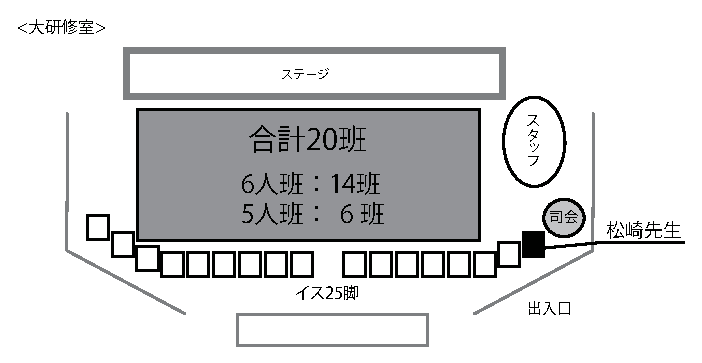
\includegraphics[scale=1.5]{./08/nyushoshiki.eps}
  \caption{入所式配置図}
  \label{nyusyosiki}
  \end{center}
\end{figure}


\subsection{必要物品}
\begin{itemize}
\item マイク:1つ
\item 靴を入れていた袋を回収する用のビニール袋:3つ
\end{itemize}

\clearpage

\subsection{各班代表者}
\begin{table}[htb]
  \begin{center}
  \begin{tabular}{|l|l||l|l||l|l||l|l||l|l|} \hline
  1班 & 伊崎 & 2班 & 生野 & 3班 & 北村 & 4班 & 丸田 & 5班 & 塩谷 \\ \hline
  6班 & 吉田 & 7班 & 青山 & 8班 & 高橋(龍) & 9班 & 石野 & 10班 & 別役  \\  \hline
  11班 & 角原 & 12班 & 新田 & 13班 & 東 & 14班 & 中島 & 15班 & 新川 \\ \hline
  16班 & 江川 & 17班 & 高島 & 18班 & 野田 & 19班 & 渡辺 & 20班 & 真壁 \\ \hline
    \end{tabular}
  \end{center}
\end{table}


\subsection{備考}
\begin{itemize}
\item 後遣隊や荷卸により班代表が揃ってない場合は,前後の班代表が整列を行う
%\item 下出は入所式開始に間に合わないため,尾辻は17班の整列を行う
\item 整列時,新入生と教職員は対面した状態で整列させる
\item 司会者は,新入生へ入所式開始前に出入り口の方を向くことを促す
\item 大研修室のキャパシティがギリギリであるため,司会と班代表が詰めて座るように促す
\item 入所式後,教員紹介のため新入生は座ったまま待機させる
\item 教員紹介が始まる前に司会者は新入生に、先生と対面に座るように促す
\item 時間の関係上,速やかに行動できるように各々がやるべきことを把握しておく
\item 最初に話す松崎先生は施設職員に向けたあいさつがある
\item 教員紹介は1人あたり1分程度にする
\item 教員紹介に来られなかった教員は司会が紹介を行う
\end{itemize}


 %\subsection{連絡事項}
% ◯◯は教員紹介終了後,報告LINEに野外炊事場に向かうことを伝える

%\include{end}


% --*- coding:utf-8-unix mode:latex -*--
%\include{Begin}
%%%%%%%%%%%%%%%%%%%%%%%%%%%%%%%%%%%%%%%%%%%%%%%%%%%%%%%%%%%%%%%%%%%%%%%%%%%%%%%

\section{野外炊事}

\subsection{日時・場所}

\begin{tabular}{p{2zw}rp{38zw}}
  日時 & : & 2019年4月5日(金) 16:20 $\sim$ 19:00\\
  場所 & : & 野外炊事場
\end{tabular}

\subsection{目的}
新入生同士及び在学生,教職員が協力して料理を作ることにより,親睦や交流をはかるきっかけにしてもらう.

\subsection{タイムスケジュール}
% 時刻は必ず4桁(00:00)で書くこと!!!
\begin{longtable}{p{3zw}p{39zw}}
  16:20 & \textbf{◎ 野外炊事場到着}\\
        %& \ \  \textbullet \ \ \underline{野外炊事統括(高島)} \\
        %& \ \  - A棟で待機し,肉を渡す準備をする \\
        & \ \  \textbullet \ \ \underline{各班スタッフ} \\
        & \ \  - 各班のプラカードが置かれている机に誘導する \\
        & \ \  - 野外炊事場で点呼が完了したら小松に報告し,本部で食器・道具・食材を受け取る \\
        & \ \  \underline{※雨天時:傘は邪魔にならない場所(机の下など)に置く} \\\\


  16:25 & \textbf{◎ 野外炊飯説明} \\
        & \ \  \textbullet \ \ 各班スタッフは席に着いたら説明があることを伝える \\
        & \ \  \textbullet \ \ 全員席に着いたら,小松は施設職員さんに説明をお願いする \\
        & \ \  \textbullet \ \ 施設職員さんより野外炊飯の説明が行われる \\
        & \ \  \textbullet \ \ 片付けの説明はよく聞いておく \\


        & \textbf{◎ アイスブレイキング} \\
        & \ \  \textbullet \ \ \underline{各班スタッフ} \\
        & \ \  - 班内の教職員,スタッフ,新入生で,自分の名前,呼んでほしいニックネーム,得意な料理,野外炊事の意気込みを言い合う(教職員のニックネームは割愛する) \\
        & \ \  - スタッフはこの意気込みから各自の力量を推測し,役割分担に役立てる \\
        & \ \  - 移動中に仲良くなったとスタッフが判断した場合は,アイスブレイキングを割愛してもよい \\\\

  16:30 & \textbf{◎ 調理開始(レシピ参照)} \\
        & \ \  \textbullet \ \ \underline{野外炊事統括(小松)} \\
        & \ \  - 班到着チェック後,本部にて食器・道具・食材の配布を行う(人数に注意) \\
        & \ \  - 全班チェック後は見回りをする \\

        & \ \  \textbullet \ \ \underline{各班スタッフ} \\
        & \ \  - 班内で役割分担を行い,調理を開始する \\
        & \ \  - 各班のスタッフは新入生が全員映るように調理風景を撮る(スマホでも可) \\
        & \ \  - 薪係は薪置き場に薪を取りに行く \\
        & \ \  - 調理が完了した班から食事をとる(食事開始前に班ごとで集合写真を撮る) \\
        & \ \  - 食事が終わり次第片付けをする \\
        & \ \  - 怪我をした場合は,2班の所に連れて行き塩谷が対応し報告スラックへ \\%(未変更)
        & \ \  - 各班,抜ける可能性がある人がいる班は2人構成,もしくは隣の班が2人構成になっているのでスタッフが抜ける場合には声をかけ,新入生だけの状態にしないようにする.\\
        & \ \  - 各班の代表は,男性教員方に野外炊事直後と22時以降のどちらでお風呂に入るか確認を取る \\
        & \ \  - 野外炊事直後に入浴を希望する男性教職員がいた場合は,報告slackに連絡する \\

  18:00 & \textbf{◎ 片付け開始}\\
        & \ \  \textbullet \ \ \underline{女性教員と先に入浴を希望する男性教員のいる班の代表} \\
        & \ \  - 食事が終了する頃に,班の代表は報告slackに連絡する \\

        & \ \  \textbullet \ \ \underline{渡辺,藤田} \\
        & \ \  - 女性教員と先に入浴希望の男性教員がいる全ての班(女性教員の班は6つ)から食事終了の連絡がきたら,それぞれの班の教職員に声をかけ,(就寝場所)に誘導する \\
        & \ \  - 渡辺が女性教員,藤田は報告slackを元に男性教員を誘導する \\
        & \ \  - 本館にて事務室でお願いし,第一・二研修室の鍵を開けてもらい,各自荷物を取りしめる \\

        & \ \  \textbullet \ \ \underline{鍵係(小谷)} \\
        % \ \  - 食事終了の連絡がきたら,事務室へ移動し,第一集会室・第二研修室・指導者棟(慎太郎と龍馬)・つどいの広間の鍵を受け取る \\
        %& \ \  - その後,第一集会室の鍵を開け待機する \\

        & \ \  - 小谷は片付けが終わり次第,先に本館に戻り,事務室でお願いして第一・二研修室を開けてもらう \\
        & \ \  - すべての荷物がなくなるまで見張りをする \\
        & \ \  - 教員紹介後見つかった忘れ物は,新入生が荷物を取りに来たとき,持ち主がいないか呼びかける \\

        & \ \  \textbullet \ \ \underline{野外炊事統括(小松)} \\
        & \ \  - 5班分の片付けが終了するころに職員の方を呼びに行く \\

        & \ \  \textbullet \ \ \underline{各班スタッフ} \\
        & \ \  - 各班スタッフは片付けが終わった時に報告slackに連絡する \\
        & \ \  - 片付けの仕方は幡多職員の指示に従う \\
        & \ \  - 食器の汚れをチェックする \\
        & \ \  - 大学の備品は一箇所に集めて机の上に置いておく \\


  18:45 & \textbf{◎ 片付けチェック}\\
        & \ \  \textbullet \ \ \underline{片付け:小松,立岩} \\
        & \ \  - 片付け終了後,各班の終了点呼を行う \\
        & \ \  - 全班完了次第,野外炊事統括(小松)は最終チェックをする.(ゴミの回収,忘れ物チェック) \\
        & \ \  - 用意した備品は全班終了後に小松が回収する \\
        & \ \  - ゴミはゴミ箱に捨てる \\

        & \ \  \textbullet \ \ \underline{各班スタッフ} \\
        & \ \  - 片付けが終了し,職員のチェックを受けた班は,野外炊事統括(小松)に直接報告する \\
        %& \ \  - ?スタッフはコンテナを持ったまま班員を第一・二研修室に誘導し,各自荷物を取る \\
        %& \ \  - 入浴係(藤田,日下)は小谷から各指導者棟の鍵を受け取る \\
        %& \ \  - ?その後,コンテナを食堂で返却し,班員をくろしお棟へ誘導する(暗いので携帯のライトアプリを使用する) \\
        & \ \  - 19班(日下),小松の荷物を,1班(生野)は立岩の荷物を第一研修室で回収し宿泊部屋に向かう \\
        & \ \  - 就寝場所への誘導終了後,報告slackに連絡する \\

        & \ \  \textbullet \ \ \underline{鍵係(小谷)} \\
        & \ \  - 第一・二研修室に忘れ物がないか確認後,自分の荷物を持って就寝場所に移動する \\
        & \ \  - 第一・二研修室に物品があった場合は,第四研修室へ入れる \\
        & \ \  \underline{※雨天時:帰り道は十分に注意する} \\
        & \ \  \underline{※雨天時:傘を忘れない} \\\\

  19:00 & \textbf{◎ 終了(完全撤退)} \\\\
\end{longtable}

\subsection{人員配置}
\subsubsection{スタッフの役割}
\begin{itemize}
  \item 救急箱担当:塩谷
  \item 野外炊事統括:小松
  %\item ?車運転:西森
  \item 各班担当:各班2名〜3名
  %\item 肉担当:高島(三浦,下出が肉を持ってくるので,その肉を置き場所を確認する)
  \item 片付け:小松,立岩
  \item 鍵担当:小谷
  \item 女性教職員誘導:渡辺
  \item 男性教職員誘導:藤田
\end{itemize}

\subsubsection{班の割り当て}
\begin{itemize}
 \item 1班(生野,貞松),2班(塩谷,立岩),3班(伊崎,西森),4班(北村,小谷)
 \item 5班(丸田,小島),6班(吉田,藤田),7班(青山,堀川),8班(別役,高橋(慎))
 \item 9班(新田,宮尾),10班(高橋(龍),斎藤),11班(横田),12班(小野)
 \item 13班(角原,以西),14班(藤田(M2)),15班(石野),16班(江川)
 \item 17班(中島,野田),18班(小松,三浦),19班(東,日下),20班(新川,藤沢)
\end{itemize}

\subsubsection{班内の役割(目安)}

準備時
\begin{itemize}
  \item 薪係:2名
  \item 食器係:2名
\end{itemize}

調理時
\begin{itemize}
  \item 火をおこす係:2名
  \item カレー係:2名
  \item 米を炊く係:1名
  %\item ?お茶を作る係:1名
  \item 皿を洗う係:1名
\end{itemize}

\subsubsection{野外炊事班}
\begin{figure}[H]
\begin{center}
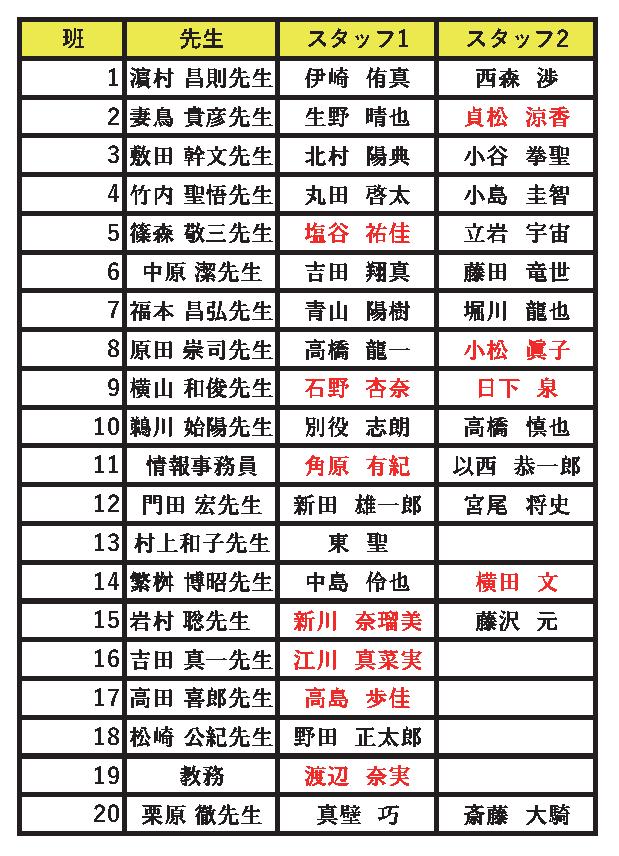
\includegraphics[scale=0.9]{./09/yagaisuijihanwake.eps}
\end{center}
\end{figure}


\subsection{必要物品(1班分)}
\begin{itemize}
  \item ピーラー:1個(20個:幡青少年自然の家)
  \item 野外炊事班のプラカード:20個(名簿入り:誘導用)
  \item 野外炊事班用紙:20枚
  \item ゴミ袋:2班で1つ(11個:幡青少年自然の家)
  \item 軍手:20組(幡青少年自然の家)
  \item ふきん:1班に1つと予備4枚(24枚) 
  \item 新聞紙:20日分(幡青少年自然の家)
  \item うちわ(予備):10個(全体)
  \item チャッカマン:2個
  \item 着火剤:2個(全体)
  \item 食器用消毒液:1班1個と予備1個(21個)
  \item ライトアプリ(足下を照らすアプリであれば指定なし)
  \item 救急箱(大学からかりる)
  \item ポリ袋(予備用)20枚
  \end{itemize}

\subsection{全体配置(晴れ)}
\begin{figure}[h]
\begin{center}
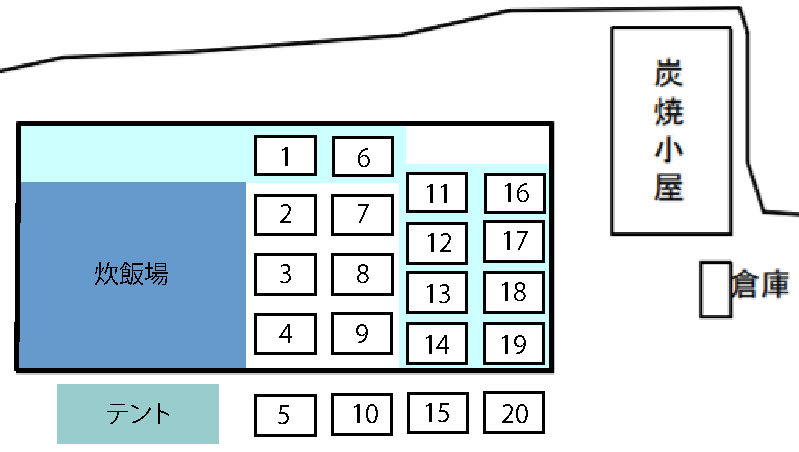
\includegraphics[width = 10cm]{./09/yagaisuiji.eps}
\label{fig:yagaihare}
\end{center}
\end{figure}

\subsection{全体配置(雨)}
\begin{figure}[h]
\begin{center}
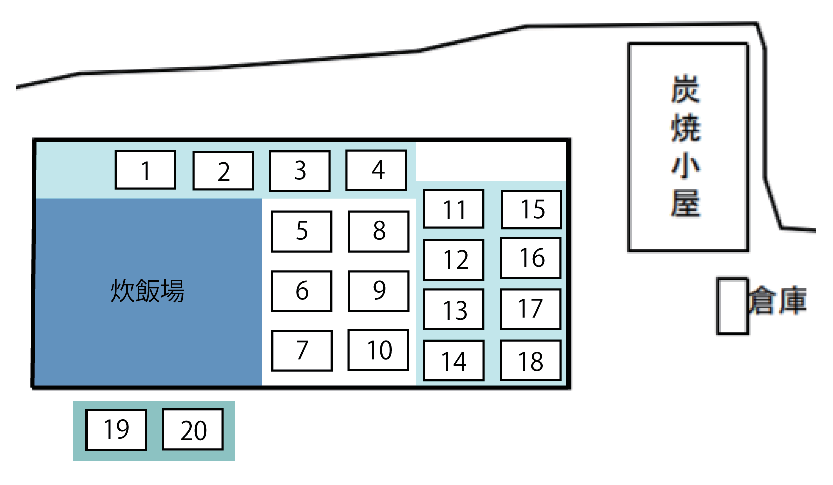
\includegraphics[width = 10cm]{./09/yagaisuijirain.eps}
\label{fig:yagaiame}
\end{center}
\end{figure}


\subsection{注意事項}
\begin{itemize}
  \item 新入生が手持ち無沙汰にならないように,人数分配を最初から終わりまで出来るだけ決めておく
  \item 時間の確認(終了時間のデッドラインや各作業の目安を確認する)
  \item 食器の個数と食材の確認
  \item 怪我に注意(火の扱い,包丁等)
  \item 食器を洗う際は,確実に汚れを落とす(点検をスムーズに行うため)
  \item 統括,各班スタッフ,新入生との「報連相」を密に行う
  %\item 鍵は担当が厳重に注意して管理する
\end{itemize}

\subsection{レシピ}
\begin{itembox}[l]{カレーのレシピ}
  \begin{enumerate}
    \item ピーラーでじゃがいも、にんじんの皮をむく
    \item 野菜は大きすぎると火が通らないので細かく薄く切る
    \item 肉は半分に切る
    \item お湯を沸かす(お茶用かつカレー非常時用に利用)
    \item 切った具材を鍋に入れ、ひたひたになるまで水を入れる(水を入れすぎない)
    \item 火にかける
    \item 沸騰まで放置する(フォーク等で刺し、じゃがいもやにんじんに穴があくかを確認する)
    \item ルーを開封前に細かく砕く
    \item 混ぜながらルーを入れる
    \item ルーが溶けたら終了
    \item カレーが濃いときはお茶用に沸かしているお湯で薄めると良い
  \end{enumerate}
\end{itembox}

\begin{itembox}[l]{ご飯のレシピ}
  \begin{enumerate}
    \item 米を研ぐ
    \item 米の表面から一差し指第2関節に行かないぐらいまで水を入れる
    \item 火にかける

    \item 最初は中火(底に火がふれるくらい)、途中で強火(はんごう全体が火に包まれるくらい)で加熱してやると美味しいご飯ができる
    \item 吹きこぼれて、吹きこぼれが乾いたら火から遠ざける(火にかけはじめて20分ほど待って吹きこぼれなかったらふたを開けて確認する)
    \item ご飯がべしゃべしゃの状態で炊けてしまったときはかまどの端っこの方(あまり火の当たらないところ)で1分ごとはんごうを回しながら水分を飛ばしてやると良い
  \end{enumerate}
※吹きこぼれている時には、絶対にふたは空けない
\end{itembox}

%\begin{itembox}[l]{お茶のレシピ}
%    \begin{enumerate}
%    \item やかんに水を入れて沸騰させる(カレーを薄めるためにお湯を使うかも知れないので早いうちからお茶っ葉を入れない)
%    \item 沸騰したらお茶っ葉をやかんに入れる
%    \item 10分ほど煮て火から遠ざける
%  \end{enumerate}
%※水を完全に沸騰させないと、味が不味くなる
%\end{itembox}

\subsection{備考}
\begin{itemize}
\item 基本的に各班代表者が報告slackへの連絡を行う
\item 火起こしの作業が遅れているときは他の班から人員を派遣する(火起こしが上手そうな人)
\item 片付けチェックで職員を呼ぶタイミングは、最初の5班から片付け終了の連絡を受けてから
\item 進行状況は随時各班のスタッフが報告slackに連絡する(見回りにいけないとこもあるかもしれないので)
\item 宮尾は翌日の朝のつどいの旗揚げの新入生(男女1名ずつ)を野外炊事中にスカウトする(なるべく目立つ子を)
\end{itemize}


%%%%%%%%%%%%%%%%%%%%%%%%%%%%%%%%%%%%%%%%%%%%%%%%%%%%%%%%%%%%%%%%%%%%%%%%%%%%%%%
%\include{End}

% 必要な項目ができた場合は適宜サブセクションを追加してください
%\include{begin}
% イベント名を記入する
\section{入浴}


% 日時と場所を記入する
% 時刻は4桁で記入すること!
\subsection{日時・場所}
\begin{tabular}{p{2zw}rp{38zw}}
  日時 & : & 2019年4月5日(金) 18:20 $\sim$ 21:00\\
  場所 & : & 大浴場,小浴場,宿泊部屋
\end{tabular}


% 目的を記入する
\subsection{目的}
新入生・先生の入浴がスムーズに行えるようにする

% イベントの概要やルールを記入する
\subsection{内容}
野外炊事から戻り,ベッドメイキング,新入生全員の入浴が終わるまでの流れを説明する \\
座談会の準備はB3以上が行い,その間にB2スタッフは入浴する \\
座談会の進行はB2が行い,B3以上で打ち合わせに参加するスタッフは22:00に間に合うように入浴する \\
他入浴していない男性スタッフは23:00以降, 女性スタッフは20:00以降入浴する \\
また,B4, 修士生を中心に,先生方の宴のお相手をする \\
他のスタッフは前日準備と座談会の準備に分かれて作業する \\
新入生が入浴終了次第,座談会に誘導する(強制しない) \\

% イベントのタイムスケジュールを記入する
% 時刻は必ず4桁(00:00)で記入すること!
% 時間の流れは途切れないように記述する!
\subsection{タイムスケジュール}
\begin{longtable}{p{3zw}p{39zw}}
  18:20 & \textbf{◎ 女性教職員と男性教職員の入浴開始} \\
        & \ \ \textbullet \ \ 女性教職員と先に入浴する男性教職員は,野外炊飯の片付けをせずに先に入浴する \\
        & \ \ \textbullet \ \ 女性教職員誘導係(渡辺)は女性教職員を小浴場に誘導する \\
        & \ \ \textbullet \ \ 男性教職員誘導係(藤田)は男性教職員を大浴場に誘導する \\
        & \ \ \textbullet \ \ 女性教職員誘導係は女性教職員に19:20までに出るように伝える \\
        & \ \ \textbullet \ \ 男性教職員誘導係は男性教職員に19:20までに出るように伝える \\
        & \ \ \textbullet \ \ 誘導後,渡辺は小浴場,藤田は大浴場の見張りをする \\
        & \ \ \textbullet \ \ 女性教職員全員の入浴が終了後,女性教職員誘導係(渡辺)は入浴終了の旨を報告slackに連絡し,宿泊部屋に移動する \\
        & \ \ \textbullet \ \ 男性教職員全員の入浴が終了後,男性教職員誘導係(藤田)は入浴終了の旨を報告slackに連絡し,宿泊部屋に移動する \\\\

  19:00 & \textbf{◎ ベッドメイキング指導開始(随時行う)} \\
        & \ \ \textbullet \ \ 各部屋のスタッフ(北村,中島,日下,塩谷)は各部屋で新入生のベッドメイキング指導を行う \\
        & \ \ \textbullet \ \ 修士生は野外炊事終了後,男性教職員のベッドメイキングを行う \\
        & \ \ \textbullet \ \ 教職員のベッドメイキングの人員が足りない場合は手の空いているB4が手伝う \\
        & \ \ \textbullet \ \ 各部屋のスタッフは新入生に,女子と男子(1回目入浴)は19:30まで,男子(2回目入浴)は20:00まで各部屋から出ないことを注意する \\
        & \ \ \textbullet \ \ 新入生自身が持参したドライヤーは使用しないように注意しておく \\
        & \ \ \textbullet \ \ 大浴場または小浴場で入浴できない新入生がいた場合は,各部屋のスタッフが連絡する \\\\

  19:30 & \textbf{◎ 1回目入浴開始} \\
        & \ \ \textbullet \ \ 各部屋のスタッフは\ref{sec:bath}節に示した入浴開始時間の5分前には入浴準備をするよう新入生を促し,浴場へ誘導して入浴を開始する \\
        & \ \ \textbullet \ \ 男子は北村,中島, 生野が,女子は塩谷,角原が誘導する \\
        & \ \ \textbullet \ \ 各部屋のスタッフが連絡を取り合い,先に女子が移動し,完了したら男子が移動を開始する \\
        & \ \ \textbullet \ \ 北村,中島は新入生と一緒に入浴開始し,生野は大浴場にて見張りをする \\
        & \ \ \textbullet \ \ 塩谷は新入生と一緒に入浴開始し,角原は小浴場にて見張りをする \\
        & \ \ \textbullet \ \ 男子新入生はベッドメイキングが終わったら各部屋で談話する(強制はしない) \\\\
        
        & \textbf{◎ 1回目入浴終了} \\
        & \ \ \textbullet \ \ 北村,塩谷はそれぞれ浴場の整理整頓と忘れ物の点検を行う \\
        & \ \ \textbullet \ \ 新入生が浴場を出るときは、見張りのスタッフが連絡を取り合い、男子と女子が一緒にならないようにする \\
        & \ \ \textbullet \ \ 生野,角原は入浴終了の旨を報告slackに連絡する \\
        & \ \ \textbullet \ \ 生野は次のグループを呼びに行く \\
        & \ \ \textbullet \ \ 新入生が各部屋に戻り次第,ベッドメイキングをするよう促す \\
        & \ \ \textbullet \ \ 翌日の荷物移動を速やかにするため,就寝前に荷造りをすませておくよう伝える \\\\

  19:45 & \textbf{◎ 2回目入浴開始} \\
        & \ \ \textbullet \ \ 丸田,吉田はベッドメイキングが終わっていない人がいれば指導する \\
        & \ \ \textbullet \ \ 男子(2回目入浴)は生野が呼びに来次第丸田,吉田, 堀川が誘導する \\
        & \ \ \textbullet \ \ 丸田,吉田は新入生と一緒に入浴開始し,堀川は大浴場にて見張りをする \\\\

        & \textbf{◎ 2回目入浴終了} \\
        & \ \ \textbullet \ \ 丸田は浴場の整理整頓と忘れ物の点検を行う \\
        & \ \ \textbullet \ \ 堀川は報告slackに入浴終了の旨を連絡し,新入生が各部屋に戻り次第,ベッドメイキングをするよう促す \\ 
        & \ \ \textbullet \ \ 堀川は次のグループを呼びに行く \\
        & \ \ \textbullet \ \ 翌日の荷物移動を速やかにするため,就寝前に荷造りをすませておくよう伝える \\\\
        
  20:00 & \textbf{◎ 3回目入浴開始} \\
        & \ \ \textbullet \ \ 高橋(龍),斎藤はベッドメイキングが終わっていない人がいれば指導する \\
        & \ \ \textbullet \ \ 男子(2回目入浴)は堀川が呼びに来次第高橋(龍),斎藤が誘導する \\
        & \ \ \textbullet \ \ 高橋(龍)は新入生と一緒に入浴開始し,斎藤は大浴場にて見張りをする \\ 
        & \ \ \textbullet \ \ 小谷が障害者用浴場の見張りを終えている場合は,斎藤は入浴し,小谷が大浴場の見張りをする \\\\

  20:30 & \textbf{◎ 入浴終了} \\
        & \ \ \textbullet \ \ 新入生は入浴終了後座談会へ向かう(強制しない)\\\\
        
        \newpage
        
        & \textbf{◎ 障害者用浴場について} \\
        & \ \ \textbullet \ \ 事前のアンケートをもとに日下,小谷は障害者用浴場に入浴する新入生を確認する \\
        & \ \ \textbullet \ \ 先に男子が入り,終わったら小谷が日下を呼びに行き,女子が入浴する \\
        & \ \ \textbullet \ \ 日下は当日に障害者用浴場での入浴を希望する新入生がいる可能性があるので,新入生女子の部屋を回って確認する \\
        & \ \ \textbullet \ \ 日下,小谷は入浴希望者を一人ずつ誘導する \\
        & \ \ \textbullet \ \ 希望者が全員入り終わるまで見張りをする \\\\
        
\end{longtable}

% イベントに必要な役割と人数を記入する
% 担当者は決定次第追記する
% 記入例 ・司会者 2人(名前1、名前2)
\subsection{人員配置}
○入浴誘導
\begin{itemize}
 \item 女子:塩谷,日下,角原
 \item 男子1:北村,中島,生野
 \item 男子2:丸田,吉田,堀川
 \item 男子3:高橋(龍),斎藤,小谷
  \item 先生(宴参加者以外):藤田
 \item 女性教職員誘導:渡辺
\end{itemize}

○ベットメイキング指導
\begin{itemize}
\item 女子:塩谷,日下
\item 男子1:北村,中島
\item 男子2:吉田,丸田
\item 男子2:高橋(龍),斎藤
\item その他スタッフ:先生のベットメイキング
\end{itemize}
% イベントに必要な物品と個数を記入する
% 記入例 ・マジックペン 10本
\subsection{必要物品}
\begin{itemize}
\item ドライヤー:8つ(洗面台4(男女2つずつ)、個室(男女2つずつ))
\item ヘアアイロン:4つ(男1女3)
%\item シャンプー
%\item ボディーソープ
\end{itemize}

\subsection{各棟入浴開始時間}
\label{sec:bath}
\begin{table}[h]
\begin{center}
\begin{tabular}{|c|c|c|c|}
\hline
 {時間}&{大浴場}&{時間}&{小浴場} \\ \hline
 18:20 & 男性教職員 & 18:20 & 女性教職員 \\ \hline
 19:30 & 新入生(男性)・男子スタッフ(B2) & 19:30 & 新入生(女性)・女性スタッフ(B2) \\ \hline
 19:45 & 新入生(男性) & & \\ \hline
 20:00 & 新入生(男性) & 20:00 & 女性スタッフ\\ \hline
 20:30 & 男性スタッフ & & \\ \hline
 22:00 & 男性教職員・男性スタッフ & & \\ \hline
\end{tabular}
\end{center}
%%\label{tab:bath}
%%\caption{各棟入浴開始時間}
\end{table}

\subsection{就寝部屋割り}
\begin{figure}[H]
\begin{center}
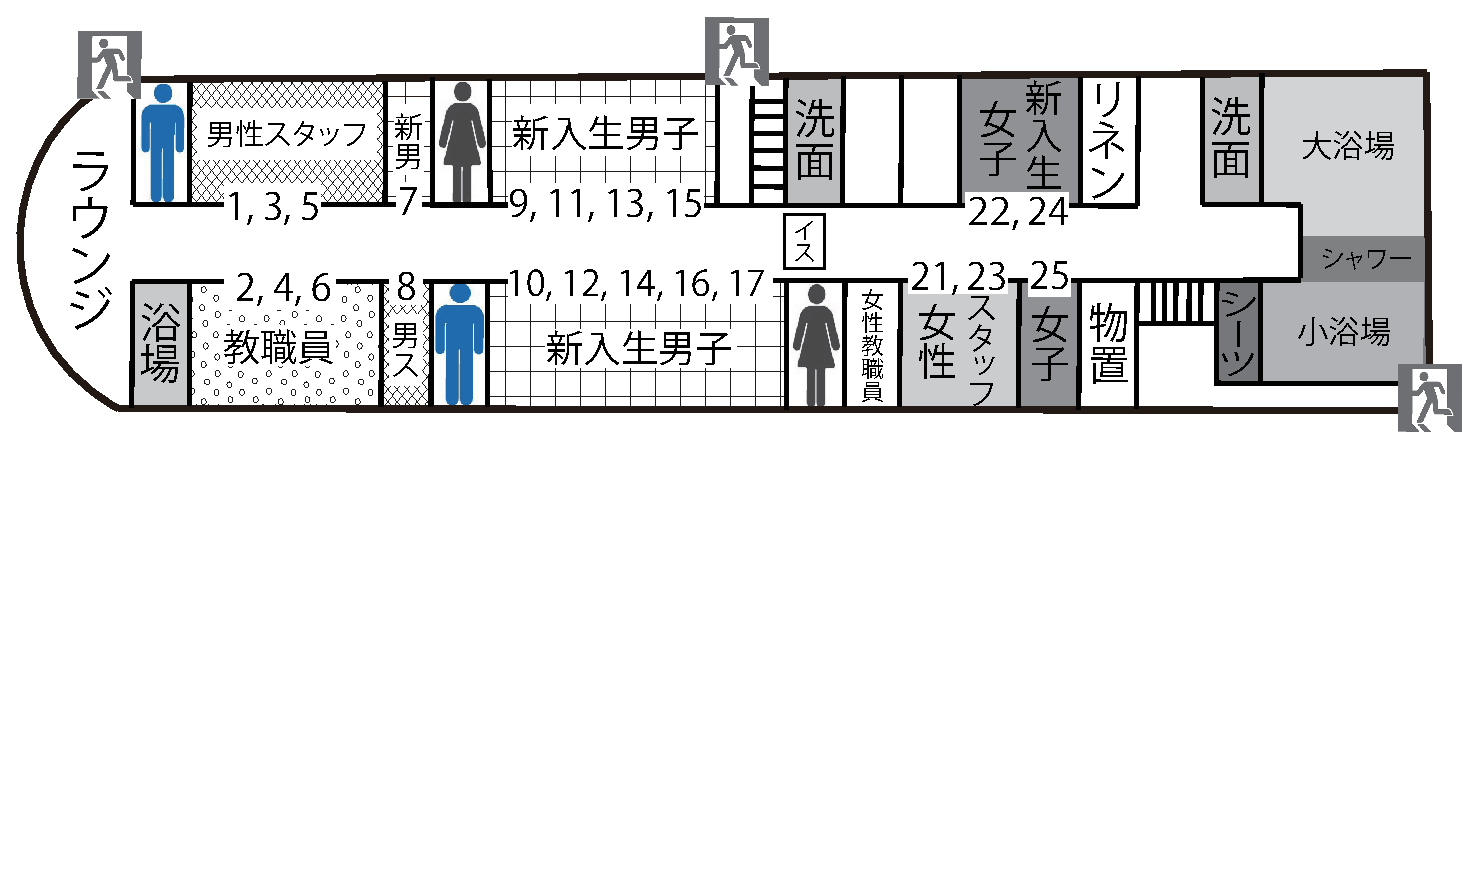
\includegraphics[scale=0.6]{./10/syushin.eps}
\vspace{-45mm}
\caption{就寝部屋割り}
\label{fig:futon_katazuke}
\end{center}
\end{figure}

% 注意事項やスタッフに周知しておくべきことがあれば記入する
\subsection{備考}
\begin{itemize}
%\item 小松(くろしお棟1担当スタッフ),宮尾(くろしお棟3担当スタッフ)は野外炊事から荷物を取りに行く時,第一集会室にいる岡本から指導者棟(龍馬・慎太郎)の鍵をもらう
%\item 基本的に,小松,宮尾が指導者棟の鍵を岡本に返却するまで,スタッフは指導者棟を使用しない
%\item その他,指導者棟の鍵が必要な人は鍵係(岡本)に連絡して鍵をもらう(指導者棟を利用する場合は,適宜報告LINEに連絡する)
%\item 時間や手間の都合上鍵を又貸しする場合は,その旨を報告LINEに報告して誰が鍵をもっているのか明確にしておく
%\item 鍵係は常に連絡がとれる状況にしておく
\item 小松,小島,西森,堀川は、夜の宴終了間近に入浴しないようにする。
\end{itemize}

% \subsection{連絡事項}
% \begin{table}[h]
% \begin{tabular}{|c|c|c|c|}
% \hline
% {報告者}&{内容}&{タイミング}&{備考}\\ \hline\hline
% Aさん & 指導者棟・慎太郎の浴場使用 & 1回目入浴開始時 & 大浴場で入浴できない新入生がいた場合のみ\\ \hline
% Bさん & 指導者棟・龍馬の浴場使用 & 1回目入浴開始時 & 小浴場で入浴できない新入生がいた場合のみ\\ \hline
% Cさん & くろしお棟1の入浴終了 & 1回目入浴終了時 & \\ \hline
% Dさん & くろしお棟3の入浴終了 & 1回目入浴終了時 & \\ \hline
% Fさん & 指導者棟・慎太郎の浴場使用 & 2回目入浴開始時 & 大浴場で入浴できない新入生がいた場合のみ\\ \hline
% Gさん & くろしお棟2の入浴終了 & 2回目入浴終了時 & \\ \hline
% \end{tabular}
% \label{tab:bath}
% \caption{各棟入浴開始時間}
%\end{table}

%\include{end}

%\include{begin}

\section{夜の宴}
\subsection{日時・場所}
\begin{tabular}{p{2zw}rp{38zw}}
  日時 & : & 2019年4月5日(金) 19:00 $\sim$\\
  場所 & : & くじら公園
\end{tabular}

\subsection{目的}
日頃の感謝の気持ちを込めて先生方にお酒の場を提供し,学生と先生方の交流を深める.学生は先生方から教育に対する想いの丈や人生の先輩としてのお話を伺うことで,今後の学生生活および社会での生活に活かす.

\subsection{タイムスケジュール}
\begin{longtable}{p{3zw}p{39zw}}
  19:00 & \textbf{◎ 宴開始} \\
        & \ \  \textbullet \ \ 野外炊事が終わり次第,くじら公園にて宴を開始する \\
        & \ \  \textbullet \ \ 入浴を希望かどうか確認し,先生は後から参加する旨を伝え,青少年の家で待機してもらう \\
	    & \ \  \textbullet \ \ 修士生は準備ととも先生方にお供し、目的達成に務める \\\\

  20:00 & \textbf{◎ 先生方の入浴} \\
	    & \ \  \textbullet \ \ ???,???が誘導し,先生方に小浴場にて入浴していただく \\
	    & \ \  \textbullet \ \ 入浴よりもお酒を優先される先生方には,入浴時間が限られている(21:00まで)ことを伝える\\\\

  ??:?? & \textbf{◎ 宴終了} \\
        & \ \  \textbullet \ \ 公園にゴミを残さないように片付けはしっかりする \\
  	    & \ \  \textbullet \ \ 状況により,青少年の家のスタッフに連絡を取り,片付けを手伝いに来てもらう \\
\end{longtable}


\subsection{人員配置}
\begin{itemize}
\item 他の作業がない満20歳以上のスタッフ
\item 喫煙スタッフ:???
\end{itemize}


\subsection{必要物品}
\begin{itemize}
  \item 酒
  \item つまみ
  \item お冷
  \item 氷
  \item 取り皿
  \item ゴミ袋
  \item クーラーボックス
  \item キッチンペーパー
  \item 紙コップ(先生方が大量に消費するため去年より大量に)
\end{itemize}


\subsection{備考}
\begin{itemize}
	\item 翌日に車を運転するあるいは早朝に仕事が割り振られているスタッフは,作業に支障をきたさないようにする
	\item 飲み過ぎにより,先生方・スタッフ・新入生に迷惑をかけない(特にスタッフは飲みすぎて明日のイベントに支障をきたす恐れがあるため飲み過ぎ厳禁)
	\item 女子スタッフは21:00をめどに,自分の部屋へ戻る(22:00には撤収)
	\item 棟内は禁煙であるため,喫煙は所定の場所へ移動する(喫煙スタッフ適宜お供に付く)
	\item ゴミを分別する
	\item 酒類のゴミ(缶や注がれた紙コップ)は,一度水洗いしてゴミ袋に入れる
	\item スタッフは率先して先生方にお酒をお注ぎする
	%\item 施設全体として原則禁酒であるため,お酒をくろしお棟4以外から持ち出さない(持ち出そうとした場合は止める)
	%\item 新入生をくろしお棟4へ侵入させない
    %\item 体調の悪い人は部屋で待機する(くろしお棟4の1階にいると飲まされる可能性があるため)
    %\item 先生方がお酒を用意してくださるのでそこまでお酒を購入しなくても良い?
\end{itemize}

%\include{end}

% 必要な項目ができた場合は適宜サブセクションを追加してください

%\include{begin}

% イベント名を記入する
\section{前日準備}


% 日時と場所を記入する
% 時刻は4桁で記入すること!
\subsection{日時・場所}
\begin{tabular}{p{2zw}rp{38zw}}
  日時 & : & 2019年4月5日(金) 19:00 $\sim$ 22:00\\
  場所 & : & 体育館
\end{tabular}


% 目的を記入する
\subsection{目的}
翌日のイベント開始前に行う準備作業を減らす.

\subsection{内容}
野外炊事が終わり担当グループの新入生を各部屋まで誘導後,ロビーに集合する \\
第4研修室から必要な機材を体育館に運び出し,小島は機材(パソコン,カメラ等)の動作確認をする \\
机,椅子を体育館に配置する \\
イベントで使う備品は第4研修室にまとめて置いておく \\
プレゼンターは体育館で生活紹介のリハーサルを行う \\
タイムスケジュールに記載しているように,20:00まで作業可能とする \\
作業が早く終了したらその時点で終了とする \\
現場は宮尾の指揮で動く \\

% イベントのタイムスケジュールを記入する
% 時刻は必ず4桁(00:00)で記入すること!
% 時間の流れは途切れないように記述する!
\subsection{タイムスケジュール}
\begin{longtable}{p{3zw}p{39zw}}
  19:00 & \textbf{◎ スタッフ集合・作業開始} \\
        & \ \ \textbullet \ \ 宮尾が報告slackに連絡する\\
        & \ \  \textbullet \ \ ロビーに集合次第,作業開始 \\\\
  22:00 & \textbf{◎ 作業終了} \\
        & \ \  \textbullet \ \ 最長作業終了時間\\
\end{longtable}


% イベントに必要な役割と人数を記入する
% 担当者は決定次第追記する
% 記入例 ・司会者 2人(名前1、名前2)
\subsection{人員配置}
\begin{itemize}
\item 鍵係:小谷
\item イベント統括:宮尾
\item 機器操作:小島
\item 総合司会:新川,貞松
\item 生活紹介リハーサル:東,高橋(慎)
\item 各イベントプレゼンター:伊崎,青山
\item Mac:宮尾,小島,東
\item Windows:高橋(慎),藤沢,小松
\end{itemize}


% イベントを実施するときに新入生や先生、スタッフがどこに配置するかを記入する
% 図があるとわかりやすい
%\subsection{全体配置}


% イベントに必要な物品と個数を記入する
% 記入例 ・マジックペン 10本
\subsection{必要物品}
\begin{itemize}
\item 机:3つ
\item 椅子:1つ
\item プロジェクタ
\item PC(小島のPCを使用)
\item カメラ(iPhoneを使用)
\item 延長ケーブル
\item スケッチブック:7冊
\item イベント班を示したプラカード:14個
\item 景品
\item 予備のPC
\item プロジェクターに接続する変換器
%\item 赤白帽:7つ
%\item ヒントを書く小さい紙:84枚
%\item ヒントをまとめる大きい紙:28枚
\item マジック:14本
\end{itemize}


% 注意事項やスタッフに周知しておくべきことがあれば記入する
\subsection{備考}
\begin{itemize}
\item 机,椅子は体育館にあるものを使用する
\item マイクの電池を確認しておく
%\item 昨年,つどいの広間の鍵を借り忘れて作業ができなかったので,鍵係の岡本は鍵を借りることを忘れない!
\item 宮尾はすぐ連絡が取れるようにスマホを常備しておく
\end{itemize}

%\include{end}



\section{夜の座談会}
\subsection{日時・場所}
日時:2019年4月5日(土)20:30〜(終わった人から順に参加してもらう)\\
\ \ \ 場所:食堂・ロビー\\
\subsection{目的}
一年生が先輩との交流を深め,学校生活で心配なことなどを聞く.
\subsection{イベント内容(概要)}
ロビーでカードゲームやボードゲームを,食堂内でブースを4つ(履修・授業ブース,フリー,サークル,バイト)用意し自由に一年生が回る.食堂では,一つのブースに
テーマに沿ったテンプレのような用紙を用意しておく
\subsection{タイムスケージュール}
20:00 \ \ \ ◎ \textbf{夜の座談会開始}\\
\hspace{15mm}・新一年生には順次参加してもらう \\
\ \ \ 21:30 \ \ \ ◎\textbf{終了}
\subsection{必要物品}
\begin{itemize}
\item ブースのテーマ用紙:12枚
\item トークテーマ用紙:30枚
\item トランプ:2つ
\item UNO:1つ
\item オリジナルすごろく(ボートゲーム):2つ
\item お菓子:いっぱい
\item サイコロ
\item 飲み物:ジュースをいっぱい
\item 紙皿
\item 紙コップ
\item 割り箸
\item サインペン
\item ウェットティッシュ:5個
\item キッチンペーパー:6個
\item ゴミ袋:6個
\end{itemize}
\subsection{人員配置}
\begin{itemize}
\item 勉強:塩谷
\item サークル:中島
\item バイト:北村
\item フリートーク:吉田
\item ゲーム:高橋,丸田
\item その他;角原,小松,渡辺,小谷,斎藤,藤田,立岩,日下,堀川
\end{itemize}
\subsection{備考}
トランプについては堀川と藤沢が,UNOを藤沢が持ってくる.(教授も参加OK)
\subsection{全体配置}
\begin{center}
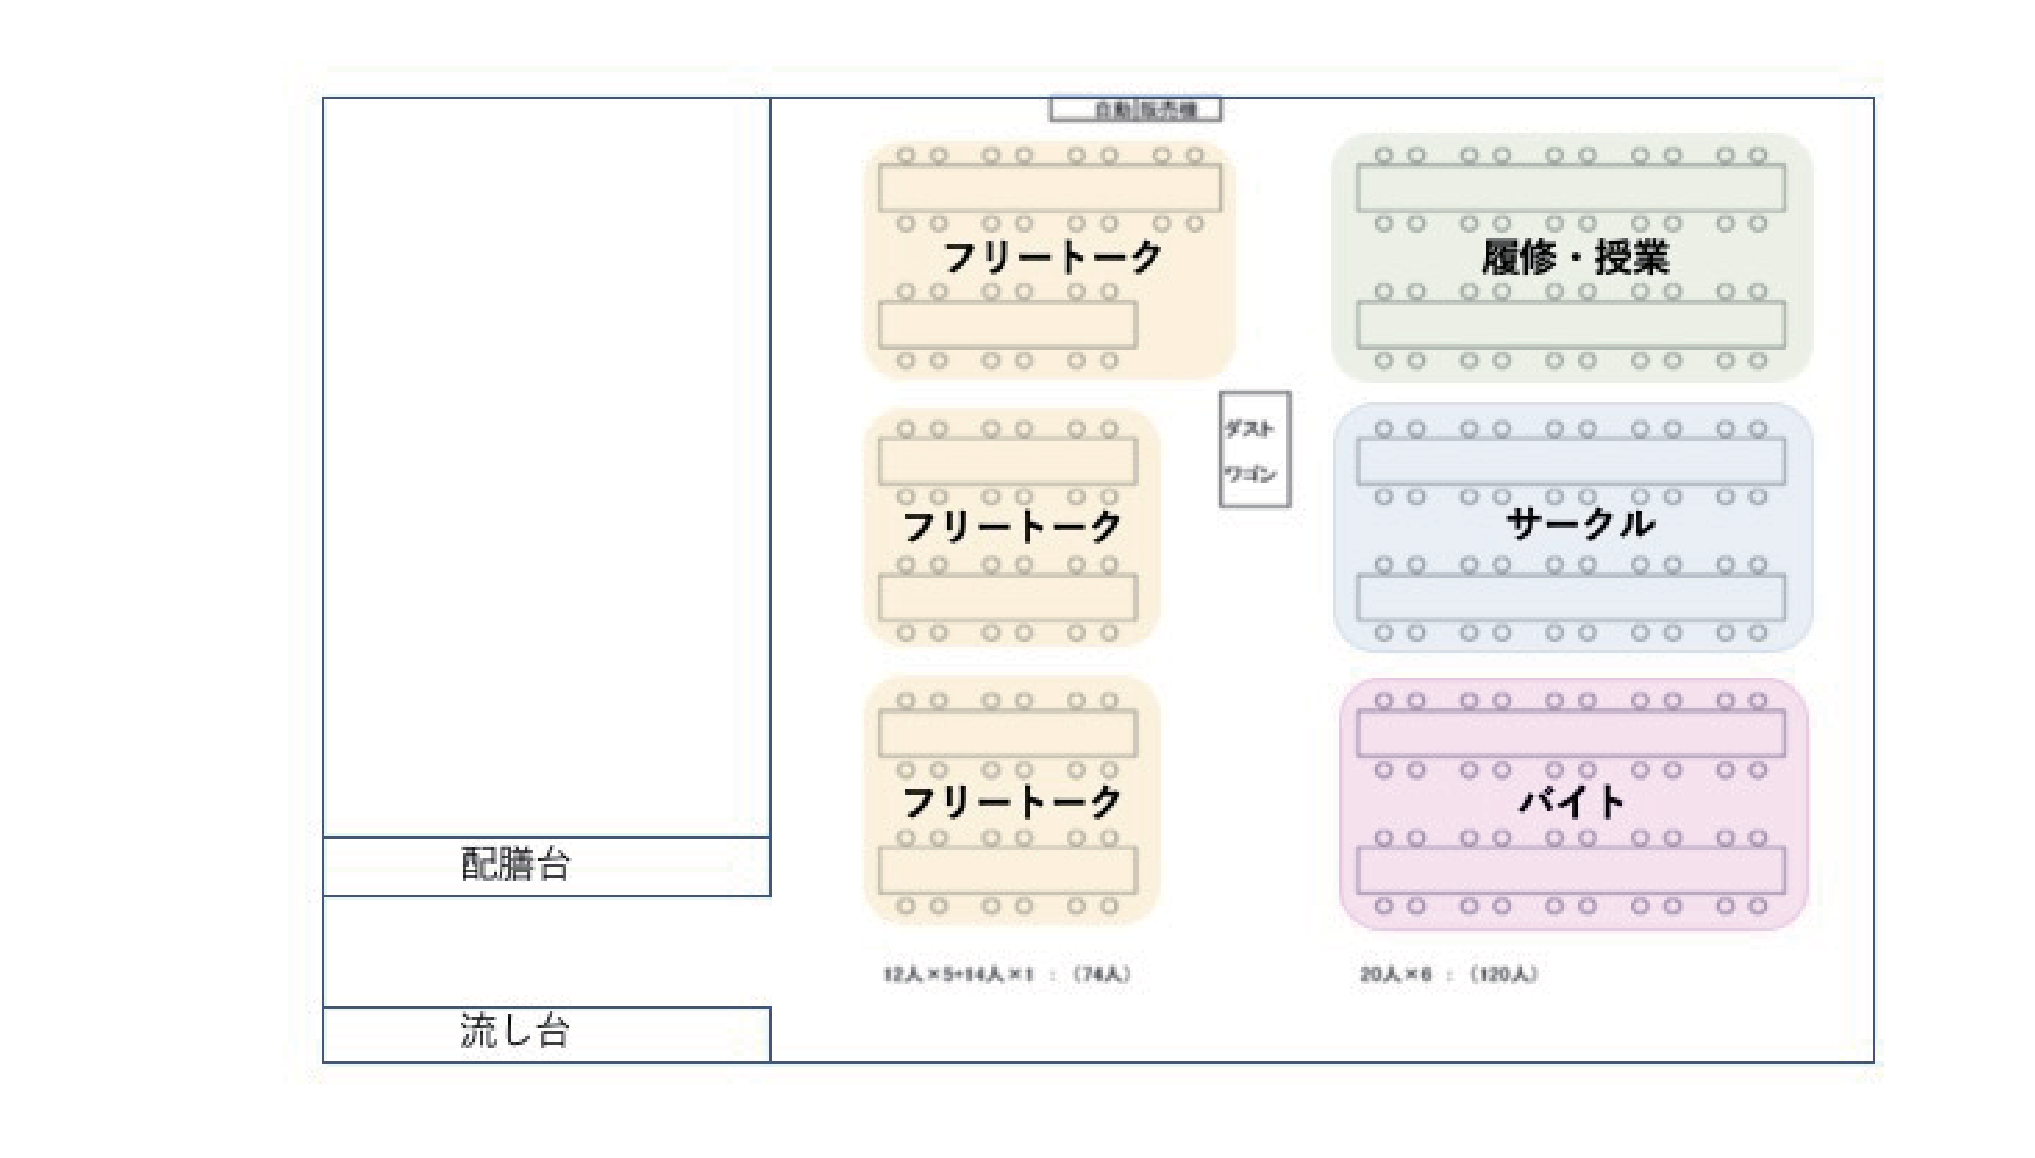
\includegraphics[width=12cm]{./13/hone.eps}
\end{center}

%\include{begin}

\section{打ち合わせ}

\subsection{日時・場所}
\begin{tabular}{p{2zw}rp{38zw}}
  日時 & : & 2019年4月5日(金) \\%22:00 $\sim$ 23:00\\
  場所 & : & 
\end{tabular}

\subsection{目的}
翌日のイベントをスムーズに行うため.

\subsection{タイムスケジュール}
\begin{longtable}{p{3zw}p{39zw}}
  22:00 & \textbf{◎集合} \\
        & \ \  \textbullet \ \ 打ち合わせに参加するメンバーは22:00に参加できるように行動する \\
        & \ \  \textbullet \ \ 宴に参加している場合は飲み過ぎないように注意する \\\\

  22:10 & \textbf{◎ 打ち合わせ開始} \\
        & \ \  \textbullet \ \ 1日目の反省,気になる点などの確認・報告をする \\
        & \ \  \textbullet \ \ 翌日のイベントを中心に一度流れを確認する \\
        & \ \  \textbullet \ \ 新入生の様子,先生方の様子などで気になることがあれば必ず報告する \\\\
        & \ \  \textbullet \ \ イベント準備を行うスタッフ(4名)は朝の集いのタイムスケジュールを確認しつつ,朝の集い中に朝食に抜けるタイミングを決める \\\\

  23:00 & \textbf{◎ 打ち合わせ終了} \\
\end{longtable}

\subsection{人員配置}
\begin{description}
%  \item 長道 横田 藤沢 生野 藤田(竜世) 野田 堀川 和田 
\end{description}

\subsection{備考}
\begin{itemize}
  %\item 野田は慎太郎に移動する際、岡本(鍵係)から慎太郎の鍵を受け取る
  \item 宴に参加しているスタッフは集合に間に合うように注意する
  \item 前日準備の進捗を確認する
\end{itemize}

%\include{end}

% 必要な項目ができた場合は適宜サブセクションを追加してください

%\include{begin}

% イベント名を記入する
\section{就寝}

% 日時と場所を記入する
% 時刻は4桁で記入すること!
\subsection{日時・場所}
\begin{tabular}{p{2zw}rp{38zw}}
  日時 & : & 2019年4月5日(金) \\%22:00 $\sim$ 23:40\\
  場所 & : & 宿泊部屋
\end{tabular}


% イベントの概要やルールを記入する

% イベントのタイムスケジュールを記入する
% 時刻は必ず4桁(00:00)で記入すること!
% 時間の流れは途切れないように記述する!
\subsection{タイムスケジュール}
\begin{longtable}{p{3zw}p{39zw}}
  22:00 & \textbf{◎ 消灯呼びかけ(1回目見回り)} \\
        & \ \  \textbullet \ \ 女子:新川\\
        & \ \  \textbullet \ \ 男子:北村\\\\

  22:30 & \textbf{◎ 2回目見回り開始} \\
        & \ \  \textbullet \ \ 女子:塩谷\\
        & \ \  \textbullet \ \ 男子:中島\\\\

  23:00 & \textbf{◎ 3回目見回り開始} \\
        & \ \  \textbullet \ \ 女子:小松\\
        & \ \  \textbullet \ \ 男子:高橋(龍)\\\\

  23:30 & \textbf{◎ 4回目見回り開始} \\
        & \ \  \textbullet \ 女子:日下\\
        & \ \  \textbullet \ \ 男子:斎藤\\\\

  23:40 & \textbf{◎ 4回目見回り終了、スタッフ就寝} \\

\end{longtable}


% イベントに必要な役割と人数を記入する
% 担当者は決定次第追記する
% 記入例 ・司会者 2人(名前1、名前2)


% イベントを実施するときに新入生や先生、スタッフがどこに配置するかを記入する
% 図があるとわかりやすい


% イベントに必要な物品と個数を記入する
% 記入例 ・マジックペン 10本

% 目的を記入する
\subsection{人員配置}
\begin{itemize}
\item 女子見張り: 新川,塩谷,小松,日下
\item 男子見張り: 北村,中島,高橋(龍),斎藤
\end{itemize}


\subsection{必要物品}
\begin{itemize}
\item 懐中電灯:4本
\end{itemize}


\subsection{注意事項}
\begin{itemize}
\item 自動販売機の使用は原則禁止する
%\item 万が一自動販売機へ行きたい新入生がいたら,自動販売機(食堂前とくろしお棟洗濯室の隣)へ誘導しその学生が買い終わるまで見張る(そのまま脱走する可能性を防ぐため)
\item 女子部屋に男子が,男子部屋に女子が行かないように見張る
\item それと同時に男性の先生方が女子部屋に,女性の先生方が男子部屋に行かないように注意する
\item その他何が起こるかわからないため,見回り時に何かあったら報告slackに連絡する
\end{itemize}

% 注意事項やスタッフに周知しておくべきことがあれば記入する
\subsection{備考}
\begin{itemize}
\item 状況に応じて見回りの回数を増やす
\item 車出し担当スタッフは優先的に就寝できるように配慮する
\item 余裕があれば宴に参加する(B3以上)
\item 当日は懐中電灯を第4研修室に置いておくため,22:00までに自分自身で取りに行き,次の日の朝戻す
\item 何かあったら報告slackで報告する
\end{itemize}

%\include{end}

% 必要な項目ができた場合は適宜サブセクションを追加してください

%\include{begin}

% イベント名を記入する
\section{起床}


% 日時と場所を記入する
% 時刻は4桁で記入すること!
\subsection{日時・場所}
\begin{tabular}{p{2zw}rp{38zw}}
  日時 & : & 2019年4月6日(土) 6:00 $\sim$ 7:10\\
  場所 & : & 宿泊棟
\end{tabular}


% イベントのタイムスケジュールを記入する
% 時刻は必ず4桁(00:00)で記入すること!
% 時間の流れは途切れないように記述する!
\subsection{タイムスケジュール}
\begin{longtable}{p{3zw}p{39zw}}
  06:00 & \textbf{◎ 新入生・先生方・スタッフ起床} \\
        & \ \ \textbullet \ \ 起床係は新入生,先生方を起こしに行く \\
        
        & \ \ \textbullet \ \ その他のスタッフは部屋の清掃,シーツ・布団の片付けを行う(6:20までにできるだけ終わらせてスタッフ全員分の荷物の運搬をできるようにする) \\
        & \ \ \textbullet \ \ 片付けが早く終わったスタッフは???車にゴミを詰め込む \\\\
        
        & \ \ \textbullet \ \ ???, ???, ???は体調が悪い人がいないか,片付けの状態,その他気付いたことを報告slackに連絡する \\
        & \ \ \textbullet \ \ 体調が悪い人がいた場合,報告slackに報告後,妻鳥先生,幡多事務室と相談する \\
        & \ \ \textbullet \ \ 新入生を起こした後はシーツ・布団の片付けの指示を出す \\
        & \ \ \textbullet \ \ 部屋の掃除を分担して行うように指示を出す \\
        & \ \ \textbullet \ \ たたみ終わったシーツは各部屋でまとめて置くように指示する \\
        & \ \  ※朝食後に時間はあるが,なるべくこの時間で片付け・清掃などできることは終わるよう円滑に指示する \\
        & \ \ \textbullet \ \ 手の空いているスタッフは廊下,トイレ,各部屋を清掃する \\\\

  06:35 & \textbf{◎ 移動開始 } \\
\end{longtable}

% イベントに必要な役割と人数を記入する
% 担当者は決定次第追記する
% 記入例 ・司会者 2人(名前1、名前2)
\subsection{人員配置}
\begin{itemize}
\item 起床係(女子):
\item 起床係(男子):
\item 起床係(男子):
\item 起床係(先生):
\item 宴のゴミの片付け:
\end{itemize}

\clearpage

% イベントに必要な物品と個数を記入する
% 記入例 ・マジックペン 10本
\subsection{布団のたたみ方}
\begin{figure}[h]
\begin{center}
\includegraphics[scale=0.5]{./16/futon_katazuke.eps}
\caption{布団のたたみ方}
\label{fig:futon_katazuke}
\end{center}
\end{figure}


% 注意事項やスタッフに周知しておくべきことがあれば記入する
\subsection{備考}
\begin{itemize}
\item 朝のつどいまでにベッド、部屋の片付けが完了しなければ朝食終了後に行う
\item スタッフはシーツのたたみ方を指導できるようにしておく
\item 体調不良者の対応を行う
\item ???, ???は先生を軽く起こして朝食の有無を聞く
\item 朝食がいらないと言われた場合,8:30には起床してもらうことを伝える
%\item 手の空いているスタッフは宴のゴミの片づけを手伝う
\item 起床係は6:35に正面広間に移動を開始することを新入生に伝える
\item 先生方が朝の集いに参加される場合は,???, ???が誘導を行う
\end{itemize}

%\include{end}

% 必要な項目ができた場合は適宜サブセクションを追加してください
%\include{begin}

% イベント名を記入する
\section{朝の集い}

% 日時と場所を記入する
% 時刻は4桁で記入すること!
\subsection{日時・場所}
\begin{tabular}{p{2zw}rp{38zw}}
  日時 & : & 2019年4月6日(土) 06:35 $\sim$ 07:20\\
  場所 & : & 正面広間(雨天時は大研修室) \\
\end{tabular}

% 目的を記入する
\subsection{目的}
規則正しい生活を実現し,国旗・所旗が掲揚されていくと同時に本日の活動を再確認し,心身共々健康になる.

\subsection{タイムスケジュール(晴天時)}
% イベントのタイムスケジュールを記入する
% 時刻は必ず4桁(00:00)で記入すること!
% 時間の流れは途切れないように記述する!
\begin{longtable}{p{3zw}p{39zw}}
  06:35 & \textbf{◎ 移動開始} \\
        & \ \ \textbullet \ \ 整列係(高橋(龍),  塩谷)は新入生の誘導開始前に正面広間に移動し,整列の準備をする \\
        & \ \ \textbullet \ \ 誘導係(中島,丸田,渡辺,横田)は宿泊棟から誘導を開始する \\
        & \ \ \textbullet \ \ 中島,渡辺は誘導開始時に報告slackに報告する \\
        & \ \ \textbullet \ \ その他のスタッフは正面広間に到着後,整列係(高橋(龍),塩谷)の指示に従って新入生を並ばせる \\\\

  06:50 & \textbf{◎ 国旗・施設旗掲揚 ラジオ体操 スタッフ代表の挨拶} \\
        & \ \ \textbullet \ \ 幡多職員の指示に従い,国旗・施設旗掲揚(北村,角原,斎藤,と新入生3名),ラジオ体操(立岩,堀川),スタッフ代表(東)の挨拶を行う \\
        & \ \ \textbullet \ \ イベント準備スタッフ(新川,貞松,小島, 宮尾)は朝の集いが始まる頃に食堂に移動し,朝食をとる \\
        & \ \ \textbullet \ \ 朝食時の食堂内誘導スタッフ(日下,堀川)は,朝の集いの終わり頃に食堂へ移動しやすい場所で待機する \\
        & \ \  ※宮尾は前日の野外炊事に国旗・所旗掲揚する新入生3名を見つけて交渉しておく \\\\

  07:00 & \textbf{◎ 食堂へ移動開始} \\
        & \ \ \textbullet \ \ 横田は朝の集い終了後,アレルギーを持っている新入生は正面広間に残り,それ以外の新入生は食堂へ移動するように指示し,報告slackに食堂へ誘導開始の旨を報告する \\
        & \ \ \textbullet \ \ 横田は(事前に顔を見て名前と一致させておくこと)アレルギーを持っている新入生に対して,朝食・昼食をとる際の注意事項(事前に調べておく)を伝え(るが食事の変更は無い),食堂に移動する \\
        %& \ \ \textbullet \ \ 最初に教職員から食堂へ行って頂くため,先生誘導係(野田,以西)は食堂までの誘導を行う(新入生は待機) \\
        & \ \ \textbullet \ \ 食堂内誘導スタッフ(日下,堀川)も急いで食堂に向かい,食堂内の各々のポジションに配置し,新入生が入ってきたら,奥から詰めて座ることを伝える \\
        & \ \ \textbullet \ \ 誘導係(中島,丸田,渡辺,横田)は食堂へ誘導を行う \\
        & \ \ \textbullet \ \ 丸田を先頭に食堂への誘導を開始し,丸田はトイレに行きたい新入生がいたら連れて行く \\
        & \ \ \textbullet \ \ 各スタッフも誘導しながら,奥からつめて座るように指示する \\
        & \ \ \textbullet \ \ 渡辺は新入生の最後尾について全員の移動を確認する \\\\

\newpage

  07:20 & \textbf{◎ 食堂への移動完了} \\
        %& \ \ \textbullet \ \ 堀川は全員が食堂に入り終えたら報告slackに報告する(堀川が新入生をトイレに誘導していないかも確認) \\\\
\end{longtable}


\subsection{タイムスケジュール(雨天時)}
\begin{longtable}{p{3zw}p{39zw}}
  06:35 & \textbf{◎ 移動開始} \\
        & \ \ \textbullet \ \ 整列係(高橋(龍),塩谷)は新入生の誘導開始前に大研修室に移動し,整列の準備をする \\
        & \ \ \textbullet \ \ 誘導係(中島,丸田,渡辺,横田)は宿泊棟から誘導を開始する \\
        & \ \ \textbullet \ \ 中島,渡辺は誘導開始時に報告slackに報告する \\
        & \ \ \textbullet \ \ その他のスタッフは大研修室に到着後,整列係(高橋(龍),塩谷)の指示に従って新入生を並ばせる\\\\

  06:50 & \textbf{◎ スタッフ代表の挨拶} \\
        & \ \ \textbullet \ \ 幡多職員の指示に従い,スタッフ代表(東)の挨拶を行う \\
        & \ \ \textbullet \ \ イベント準備スタッフ(新川,貞松,小島,宮尾)は朝の集いが始まる頃に食堂に移動し,朝食をとる \\
        & \ \ \textbullet \ \ 朝食時の食堂内誘導スタッフ(日下,堀川)は,朝の集いの終わり頃に食堂へ移動しやすい場所で待機する \\\\

  07:00 & \textbf{◎ 食堂へ移動開始} \\
        & \ \ \textbullet \ \ 横田は挨拶終了後,アレルギーを持っている新入生はその場に残り,それ以外の新入生は食堂へ移動するように指示し,報告slackに食堂へ誘導開始の旨を報告する \\
        & \ \ \textbullet \ \ 横田は(事前に顔を見て名前と一致させておくこと)アレルギーを持っている新入生に対して,朝食・昼食をとる際の注意事項(事前に調べておく)を伝え(るが食事の変更は無い),食堂に移動する \\
        %& \ \ \textbullet \ \ 最初に教職員から食堂へ行って頂くため,先生誘導係(野田,以西)は食堂までの誘導を行う(新入生は待機) \\
        & \ \ \textbullet \ \ 食堂内誘導スタッフ(日下,堀川)も急いで食堂に向かい,食堂内の各々のポジションに配置し,新入生が入ってきたら,奥から詰めて座ることを伝える \\
        & \ \ \textbullet \ \ 誘導係(中島,丸田,渡辺,横田)は食堂へ誘導を行う \\
        & \ \ \textbullet \ \ 丸田を先頭に食堂への誘導を開始し,丸田はトイレに行きたい新入生がいたら連れて行く \\ %(トイレは浴場横のものを使用する)
        & \ \ \textbullet \ \ 各スタッフは誘導しながら,奥からつめて座るように指示する \\
        & \ \ \textbullet \ \ 渡辺は新入生の最後尾について全員の移動を確認する \\\\

 07:10  & \textbf{◎ 食堂への移動完了} \\
       %& \ \ \textbullet \ \ 堀川は全員が食堂に入り終えたら報告slackに報告する(堀川が新入生をトイレに誘導していないかも確認) \\\\
\end{longtable}

% イベントに必要な役割と人数を記入する
% 担当者は決定次第追記する
% 記入例 ・司会者 2人(名前1、名前2)
\newpage
\subsection{人員配置}
\begin{itemize}
\item 誘導係:中島,丸田,渡辺,横田
\item 整列係:高橋(龍),塩谷
\item ラジオ体操のお兄さん(晴天時):立岩,堀川
\item 旗揚げ係(晴天時): 北村,角原,斎藤,野外炊事に宮尾がスカウトした新入生3名
\item スタッフ代表の挨拶:東
\item 食堂内での誘導係:日下,堀川
\item イベント準備スタッフ:新川,貞松,宮尾,小島
\end{itemize}



\subsection{全体配置}
\begin{figure}[h]
\begin{center}
\vspace{-5mm}
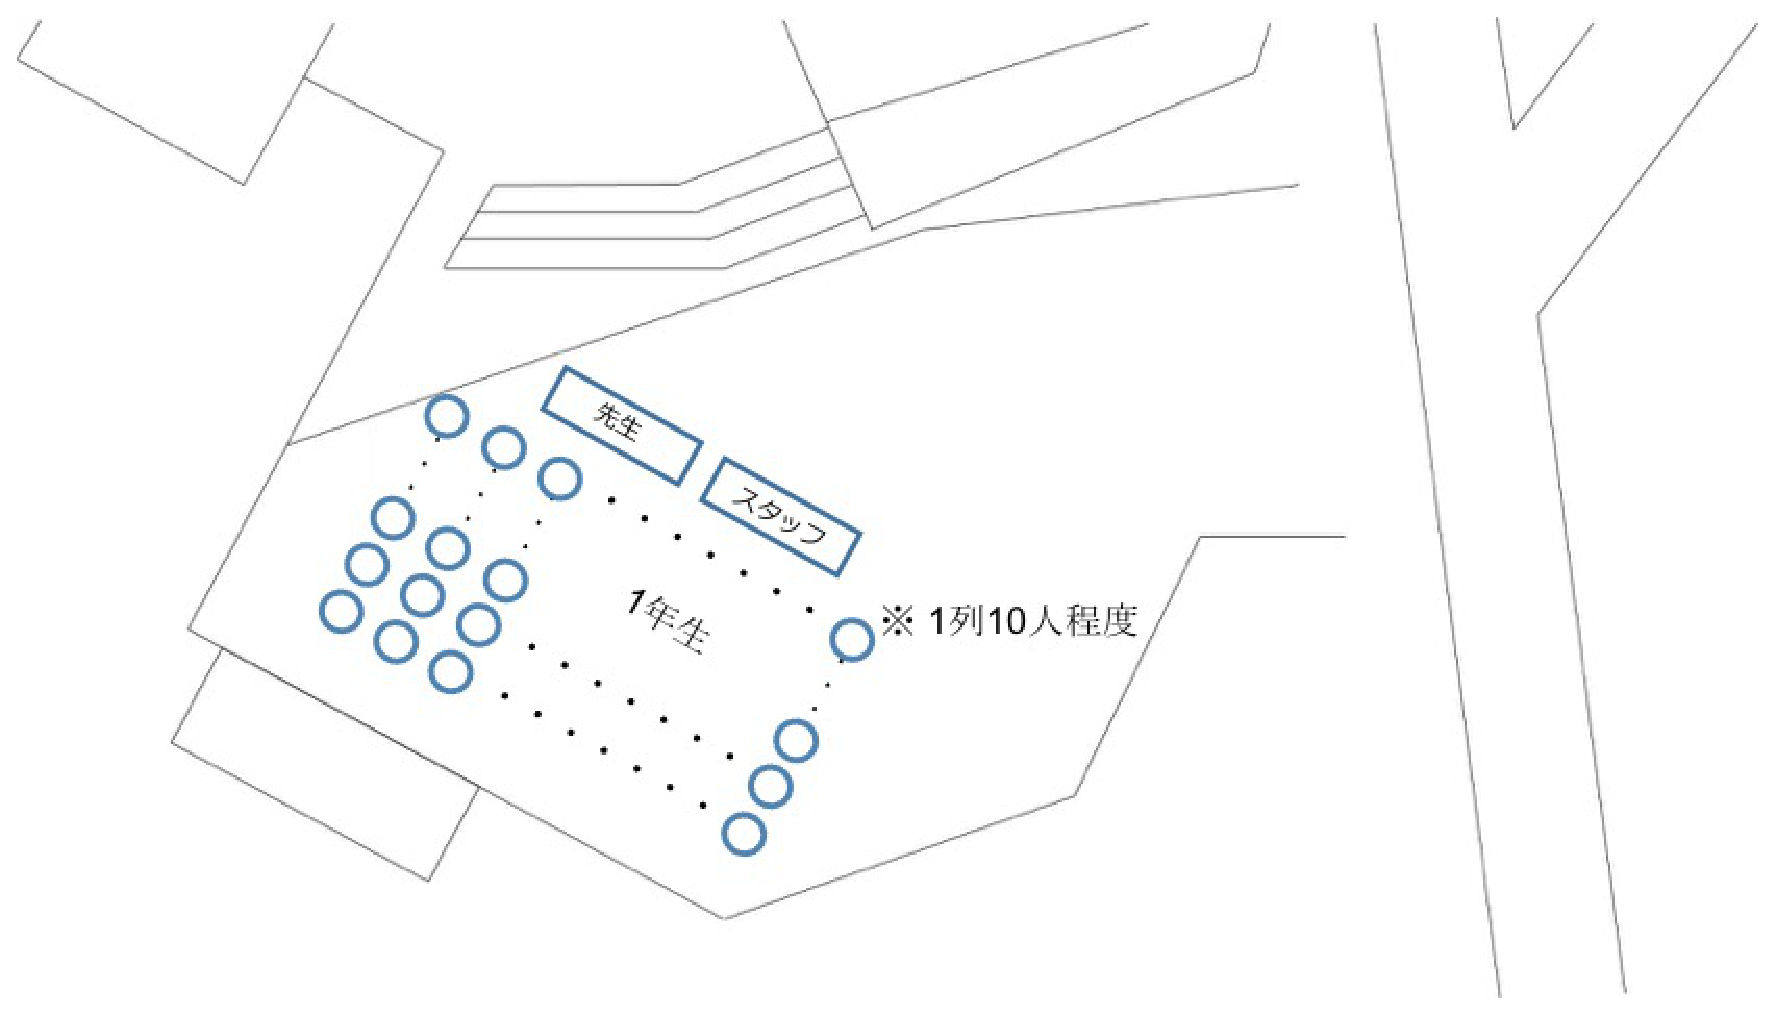
\includegraphics[scale=1.0]{./17/asanotudoihaiti.eps}
\caption{正面広間}
\end{center}
\end{figure}

\subsection{誘導経路}
\begin{figure}[H]
\begin{center}
  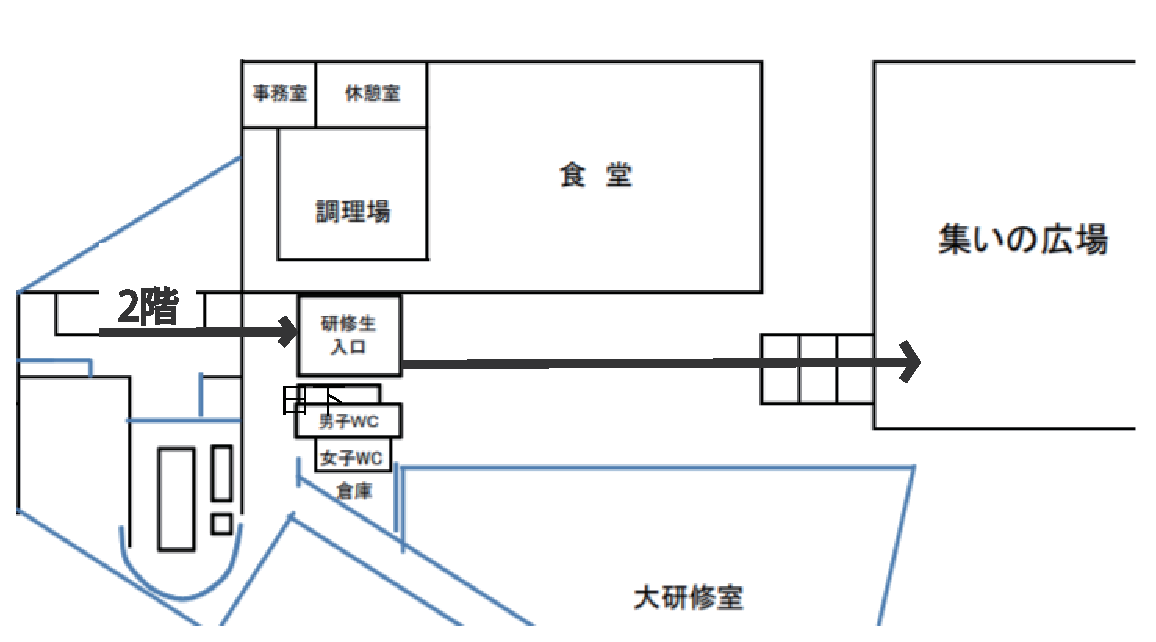
\includegraphics[scale=0.6]{./17/asanozu.eps}
\end{center}
\end{figure}


%\subsection{備考}
%人員に入っていないスタッフも朝の集いに参加する

%\subsection{連絡事項}
%\begin{table}[htb]
%\begin{tabular}{|l|c|c|} \hline
%報告者 & 内容 & タイミング \\ \hline \hline
 %& くろしお棟1誘導開始 & 7:10(誘導開始時)  \\ \hline
 %&  くろしお棟2誘導開始 & くろしお棟1退出後 \\ \hline
 %&  くろしお棟3誘導開始 & くろしお棟2退出後  \\ \hline
 %&  くろしお棟4誘導開始 & くろしお棟3退出後 \\ \hline
 %&  食堂へ誘導開始 & 自身のスタッフ代表挨拶終了後 \\ \hline

%\end{tabular}
%\end{table}

%\include{end}

% --*- coding:utf-8-unix mode:latex -*--

%%%%%%%%%%%%%%%%%%%%%%%%%%%%%%%%%%%%%%%%%%%%%%%%%%%%%%%%%%%%%%%%%%%%%%%%%%%%%%%
%\include{begin}

\section{朝食}

\subsection{日時・場所}

\begin{tabular}{p{2zw}rp{38zw}}
  日時 & : & 2019年4月6日(土) 07:20 $\sim$ 08:30\\
  場所 & : & 食堂・宿泊棟
\end{tabular}


\subsection{タイムスケジュール}
% 時刻は必ず4桁(00:00)で書くこと!!!
\begin{longtable}{p{3zw}p{39zw}}
  07:20 & \textbf{◎ 朝食開始} \\
        & \ \  \textbullet \ \ 準備スタッフ \\
        & \ \ \ \ \ - 朝食をとり次第,宿泊棟に移動し,自分の荷物をまとめる \\
        & \ \ \ \ \ - (新川,貞松,宮尾,小島)は荷物の準備ができ次第,事務室でお願いし,第一・二・四研修室の鍵を開けてもらう \\
        & \ \ \ \ \ - 自分の荷物を第一・二研修室に置き,第四研修室で物品を確保し,体育館に移動する \\
        %& \ \ \ \ \ - 和田は第二集会室,つどいの広間の順で鍵を開ける \\

        & \ \ \ \ \ - 8:15までには体育館に移動し,イベント物品の配置と打ち合わせを行う \\

        & \ \ \textbullet \ \ 誘導を行うスタッフ \\
        & \ \ \ \ \ - 朝のつどいの終了と同時に食堂内で誘導を行うスタッフは急いで食堂に向かって食堂の中の各々のポジションに配置し,奥から詰めて座ることを伝える \\
        %& \ \ \ \ \ - 藤沢を先頭に誘導開始する \\
        & \ \ \ \ \ - 丸田は誘導終了後,お手洗いに行きたい学生がいれば連れて行く \\ %(お手洗いは,浴場横のお手洗いを使用する)
        %& \ \ \ \ \ - 日下は新入生の列の中間あたりで誘導を行ない,食堂につき次第食堂内の誘導を行う \\
        & \ \ \ \ \ - 渡辺は新入生の一番後ろについて行き,新入生全員が食堂に入ったら(丸田が新入生をトイレに誘導していないかも確認)朝食をとる \\
        & \ \ \ \ \ - 各スタッフも誘導しながら奥から詰めて座るように指示する \\
        & \ \ \ \ \ - 堀川は新入生が食堂に全員入ったら報告slackに連絡する \\
        & \ \ \ \ \ - 基本的にスタッフは早めに朝食をとり,補助に回る \\\\

 08:30 & \textbf{◎ 朝食終了(新入生,食堂で仕事のないスタッフ)} \\
        & \ \ \textbullet \ \ 食事を済ませたら各自宿泊棟に戻り,片付けが終わっていなければ片付けの続きを行う \\
\end{longtable}



\subsection{人員配置}
\begin{itemize}
\item 誘導係:中島,丸田,渡辺,横田
\item 食堂内での誘導:日下,堀川
\item イベント準備スタッフ:新川,貞松,宮尾,小島
  \item 先生の誘導:野田,以西
\end{itemize}



\subsection{備考}
\begin{itemize}
\item イベントスタッフは朝食を早めにとる
\item イベント物品は第四研修室に置いている
\item 美味しく食べる


\end{itemize}

%\include{end}

%%%%%%%%%%%%%%%%%%%%%%%%%%%%%%%%%%%%%%%%%%%%%%%%%%%%%%%%%%%%%%%%%%%%%%%%%%%%%%%

% 必要な項目ができた場合は適宜サブセクションを追加してください
%\include{begin}

% イベント名を記入する
\section{朝食後の動き}

% 日時と場所を記入する
% 時刻は4桁で記入すること!

\subsection{日時・場所}
\begin{tabular}{p{2zw}rp{38zw}}
  日時 & : & 2019年4月6日(土) 08:30 $\sim$ 09:00\\
  場所 & : & 本館, 体育館
\end{tabular}

% 目的を記入する
\subsection{目的}
本館から体育館までの新入生の移動をスムーズに行い,イベント運営を円滑に行えるようにする

\subsection{タイムスケジュール}
\begin{longtable}{p{3zw}p{39zw}}
   08:30 & \textbf{◎ 宿泊場所片付け} \\
         & \ \ \textbullet \ \ 食事を済ませたら各自宿泊部屋に戻り,片付けが終わっていなければ片付けの続きを行う \\
         & \ \ \textbullet \ \ 誘導係(中島,丸田,渡辺,横田)は,新入生から部屋の片付けが終わっていないと報告があった場合,
         							朝食をとった後で宿泊部屋に向かい,片付けの指示を行う(08:45まで) \\
         & \ \ \textbullet \ \ 日下,堀川は最後の人が出るまで食堂内で待機する \\
         & \ \ \textbullet \ \ 堀川は食堂の片付けが終わり次第報告slackに連絡し,宿泊部屋に戻る \\
         & \ \ \textbullet \ \ 廊下,トイレ等の掃除は新入生にしてもらい,手の空いているスタッフは手伝う \\
         & \ \ \textbullet \ \ 片付けのチェック係(藤田(B3),高島)は,廊下,トイレ等の掃除を指示し,新入生各部屋の確認をする \\\\
         
   08:40 & \textbf{◎ プラカードの準備} \\
        & \ \  \textbullet \ \ 体育館でプラカードを持つスタッフ(塩谷,石野,角原,吉田,別役,北村,小松,藤沢,江川,東,高橋(慎),新田,立岩,斎藤,藤田(B3),生野)は,第一・二研修室に自分の荷物を置き,体育館へ行く \\
        & \ \  \textbullet \ \ その後,19.5節の表に従って,各班のプラカードを持つ\\\\

  08:45 & \textbf{◎ 体育館に移動開始} \\
        & \ \ \textbullet \ \ 本館2階には戻れないため,残りのスタッフは荷物を全て持って本館1階へ降りる(その旨を新入生にも伝える) \\
        & \ \ \textbullet \ \ スタッフ・新入生共に,バスの号車ごとに分けて,荷物を第一・二研修室に置く(19.6参照) \\
        & \ \ \textbullet \ \ 体育館に移動する前に,本館から体育館への誘導係(中島,丸田,渡辺,横田)は,新入生に体育館にしおりと筆記用具を持っていくように伝える \\
        & \ \ \textbullet \ \ 本館から体育館への誘導係(中島,丸田,渡辺,横田)は荷物を置いた新入生から順に誘導する \\
        & \ \ \textbullet \ \ その他のスタッフは付いていき,誘導の補助を行う \\
        & \ \ \textbullet \ \ 小野,藤田(M2)は教職員に,荷物を研修室に置いてから,体育館へ向かうという旨を伝える \\
        & \ \ \textbullet \ \ 小谷は全員が荷物を入れ終わったら事務室へ行き,第一・二・四研修室の鍵を閉めてもらう \\\\

        &\textbf{◎ 体育館に移動開始(雨天時)}\\
        & \ \ \textbullet \ \ 上記の点に加えて新入生や先生に傘を出すことを促し,体育館の出入り口で傘を傘立てにいれるか,または壁にかける \\\\

  08:50 & \textbf{◎ 各班プラカード係待機} \\
        & \ \ \textbullet \ \ プラカードを持つスタッフはこの時間までに各班番号のプラカードを持ち,図\ref{fig:ice}に示した位置に待機しておく \\
        & \ \ \textbullet \ \ 誘導係の誘導の下,新入生が到着したら声掛けをしながら新入生を誘導し,グループの新入生が揃ったら円になって座らせる \\
        & \ \ \textbullet \ \ 食堂から新入生や先生方を誘導してきたスタッフは速やかに自分の班に移動する \\\\

  09:00 & \textbf{◎ 移動終了・イベント開始}  \\\\
\end{longtable}


% イベントに必要な役割と人数を記入する
% 担当者は決定次第追記する
% 記入例 ・司会者 2人(名前1、名前2)
\vspace{-3mm}
\subsection{人員配置}
\begin{itemize}
\item 食堂の片付け:日下,堀川
\item 部屋の片付けチェック:藤田(B3),高島
\item 誘導係:中島,丸田,渡辺,横田
\item 体育館でプラカードを持つ係:塩谷,石野,角原,吉田,別役,北村,小松,藤沢,江川,東,高橋(慎),新田,立岩,斎藤,藤田(B3),生野
\end{itemize}

\subsection{各班プラカードとスタッフの対応}
\begin{table}[h]
\begin{center}
\label{sec:card}
\begin{tabular}{|c|c||c|c||c|c||c|c|}
\hline
{班}&{スタッフ}&{班}&{スタッフ}&{班}&{スタッフ}&{班}&{スタッフ} \\ \hline\hline
1 & 塩谷 & 5 & 別役 &  9 & 江川 & 13 & 立岩 \\ \hline
2 & 石野 & 6 & 北村 & 10 & 東 & 14 & 斎藤 \\ \hline
3 & 角原 & 7 & 小松 & 11 & 高橋(慎) & 15 & 藤田(B3) \\ \hline
4 & 吉田 & 8 & 藤沢 & 12 & 新田 &16 & 生野 \\ \hline
\end{tabular}
\end{center}
\end{table}

\subsection{第一・二研修室の荷物配置}
\begin{figure}[H]
\begin{center}
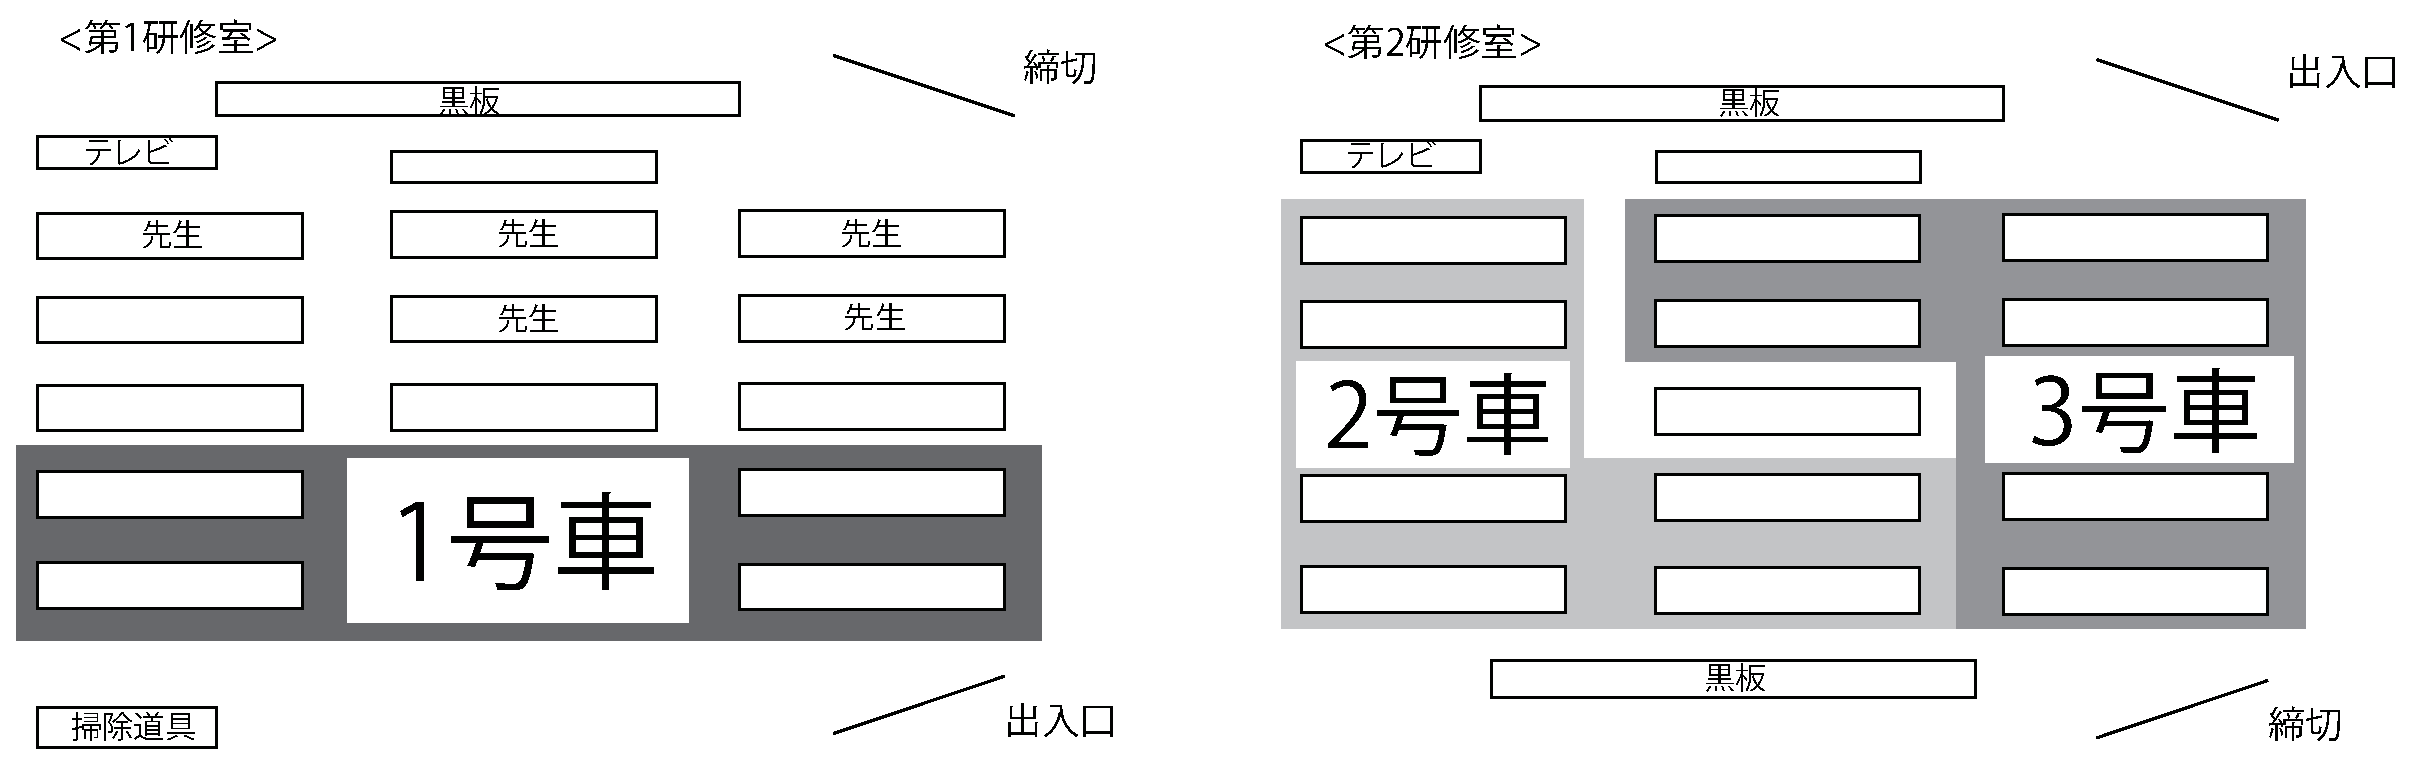
\includegraphics[scale=0.4]{./19/busnimotsu.eps}
\end{center}
\end{figure}

\vspace{-3mm}
\subsection{イベントの班分け}
%1班(真壁, 生野(イ)), 2班(石野, 小松), 3班(高島, 小野(生)), 4班(江川, 藤田(竜世)(イ)), 5班(別役, 明神), 6班(横井, 藤沢(ア), 横田(総)), 7班(東, 堀川(ア)), 8班(高橋(果), 立岩), 9班(小谷, 上村), 10班(日下, 藤田(竜貴)), 11班(角原, 野田), 12班(松尾, 以西(生)), 13班(平松, 渡辺), 14班(徳石, 岡本), 15班(高橋(錬), 長通(総)), 16班(南部, 宮尾)
\begin{figure}[H]
\begin{center}
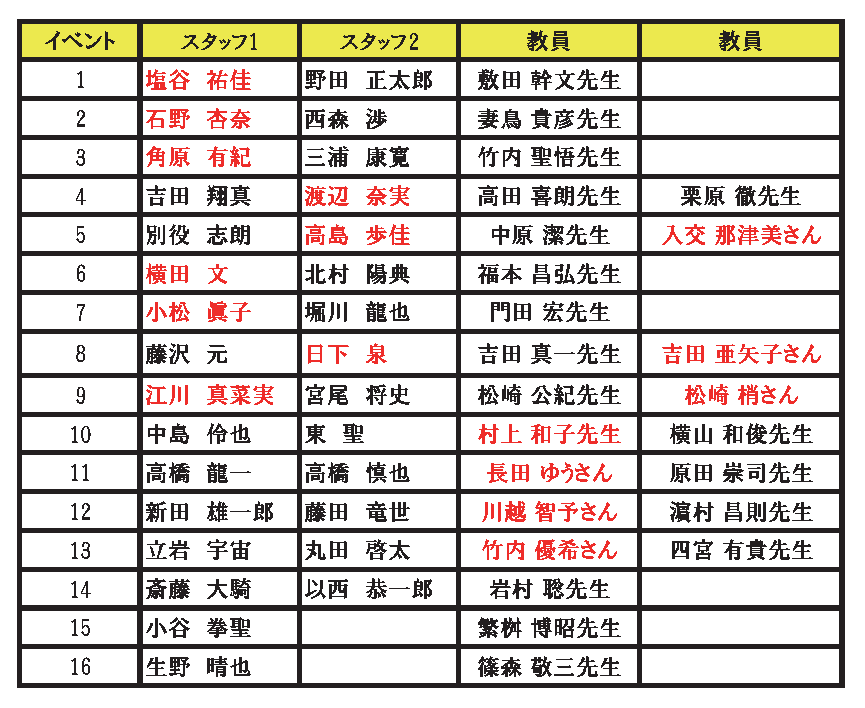
\includegraphics[scale=0.8]{./19/event_hanwake.eps}
\label{fig:Eventhanwake}
\caption{イベントの班分け図}
\end{center}
\end{figure}


%\subsection{備考}
%\begin{itemize}
%\end{itemize}

%\include{end}

%\include{begin}

\section{イベント中裏方動き}

\subsection{日時・場所}
\begin{tabular}{p{2zw}rp{38zw}}
  日時 & : & 本館2階
\end{tabular}

\subsection{目的}
2日目のイベントの裏で,円滑に退所出来るように宿泊棟の整頓を行う

\subsection{タイムスケジュール}
% 時刻は必ず4桁(00:00)で書くこと!!!
\begin{longtable}{p{3zw}p{39zw}}
 

  08:50 & \textbf{◎ シーツ運び} \\
        & \ \ \textbullet \ \ 教職員に荷物と体育館へ向かうことについて伝達後,作業を始める \\
        & \ \ \textbullet \ \ 全員が体育館に移動したら,シーツをシーツ置き場に返却する \\\\
        
  09:00 & \textbf{◎ 退所点検} \\
        & \ \ \textbullet \ \ M2は事務室に職員を呼びに行く \\
        & \ \ \textbullet \ \ 退所点検終了次第,報告slackに,体育館に向かう旨を伝え向かう \\
        & \ \ \textbullet \ \ 終了次第イベント班15,16 に参加する\\
\end{longtable}


\subsection{人員配置}
\begin{itemize}
\item 裏方:M2
\end{itemize}

\subsection{退所点検}
\begin{itemize}
\item シーツ・枕カバをきれいにたんでおく
\item 寝具・備品(ハンガー等)は元通りにする
\item 窓は閉めて,カーテンは開けて留めておく
\item 室内・廊下の掃除をし,ゴミ箱のゴミは研修生入り口のゴミ置き場に分別して処理する
\item 電気・エアコンの消し忘れをしない
\end{itemize}


\subsection{備考}
\begin{itemize}
  \item 作業終了後は体育館に入り,後ろで待機する
  \item 忘れ物を発見した場合は,宮尾に報告し,体育館まで運ぶ
  \item 忘れ物があった場合,司会はイベントの休憩時間等に忘れ物があったことをアナウンスする
\end{itemize}

%\include{end}



% 必要な項目ができた場合は適宜サブセクションを追加してください

%\include{begin}
\documentclass[a4j,titlepage]{jarticle}
\usepackage[dvipdfmx]{graphicx,epsfig}

\usepackage{longtable}

\usepackage{textcomp}



\usepackage{float}

\usepackage{ascmac}
\usepackage{fancybox}
\usepackage{url}


\begin{document}

% イベント名を記入する
\section{アイスブレイキング}


% 日時と場所を記入する
% 時刻は4桁で記入すること!
\subsection{日時・場所}
\begin{tabular}{p{2zw}rp{38zw}}
  日時 & : & 2019年4月6日(土) 09:00 $\sim$ 09:40\\
  場所 & : & つどいの広場
\end{tabular}


% 目的を記入する
\subsection{目的}
  本イベントでは,「ワードウルフ」というゲームを通して打ち解け合い,楽しく話し合う環境を作ることで,これからのスケジュールを楽しんでもらうことを目的とする.

% イベントの概要やルールを記入する
\subsection{イベント内容}
  ワードウルフは制限時間内でグループの中での少数派の人を探すゲームである.自分が多数派か少数派かわからない状況でグループ内で話し合い,少数派と多数派の意見のズレを探して誰が少数派かを予測する.自分が少数派だと思ったら少数派だと知られないように多数派になりすまし,上手く立ち振る舞う.

% イベントのタイムスケジュールを記入する
% 時刻は必ず4桁(00:00)で記入すること!
% 時間の流れは途切れないように記述する!
\subsection{タイムスケジュール}
\begin{longtable}{p{3zw}p{39zw}}
  09:00 & \textbf{◎ 整列} \\
        & \ \  各スタッフは新入生と教員方を誘導して整列する. 整列完了後,その場に座る.(図\ref{fig:ice}を参照) \\
        & \ \  次の仕事を控えたスタッフは準備に入る. \\
        & \ \  整列を終え,全員が座ったら頃合いを見て司会は話し始める.\\

  09:03 & \textbf{◎ アイスブレイクの説明}\\
        & \ \  パワーポイントを用いてアイスブレイクの説明を行う.\\
        & \ \  分からない新入生がいたら各班のスタッフが補足説明を行う.\\
        & \ \  スタッフから順番に自己紹介をしていく(名前,出身県,100万あったら何したい). \\

  09:10 & \textbf{◎ ワードウルフの説明}\\
        & \ \  パワーポイントを用いてワードウルフの説明を行う.\\
        & \ \  分からない新入生がいたら各班のスタッフが補足説明を行う.\\

  09:14 & \textbf{◎ ワードウルフの開始}\\
        & \ \  スタッフがお題の紙を配る.\\
        & \ \  プレゼンターが時間を計り,7分間話し合って少数派を見つける.\\
        & \ \  その後,自分のお題の紙を全員で見せ合い,答え合わせをする.\\

  09:25 & \textbf{◎ アイスブレイキング終了し休憩(10分間)}\\

\end{longtable}


% イベントに必要な役割と人数を記入する
% 担当者は決定次第追記する
% 記入例 ・司会者 2人(名前1、名前2)
\subsection{人員配置}
\begin{itemize}
\item 司会:横田,長通
\item プレゼンター:藤沢,堀川
\item プラカード:各班スタッフ代表
\end{itemize}


% イベントを実施するときに新入生や先生、スタッフがどこに配置するかを記入する
% 図があるとわかりやすい
\subsection{全体配置}
\begin{figure}[h]
  \begin{center}
    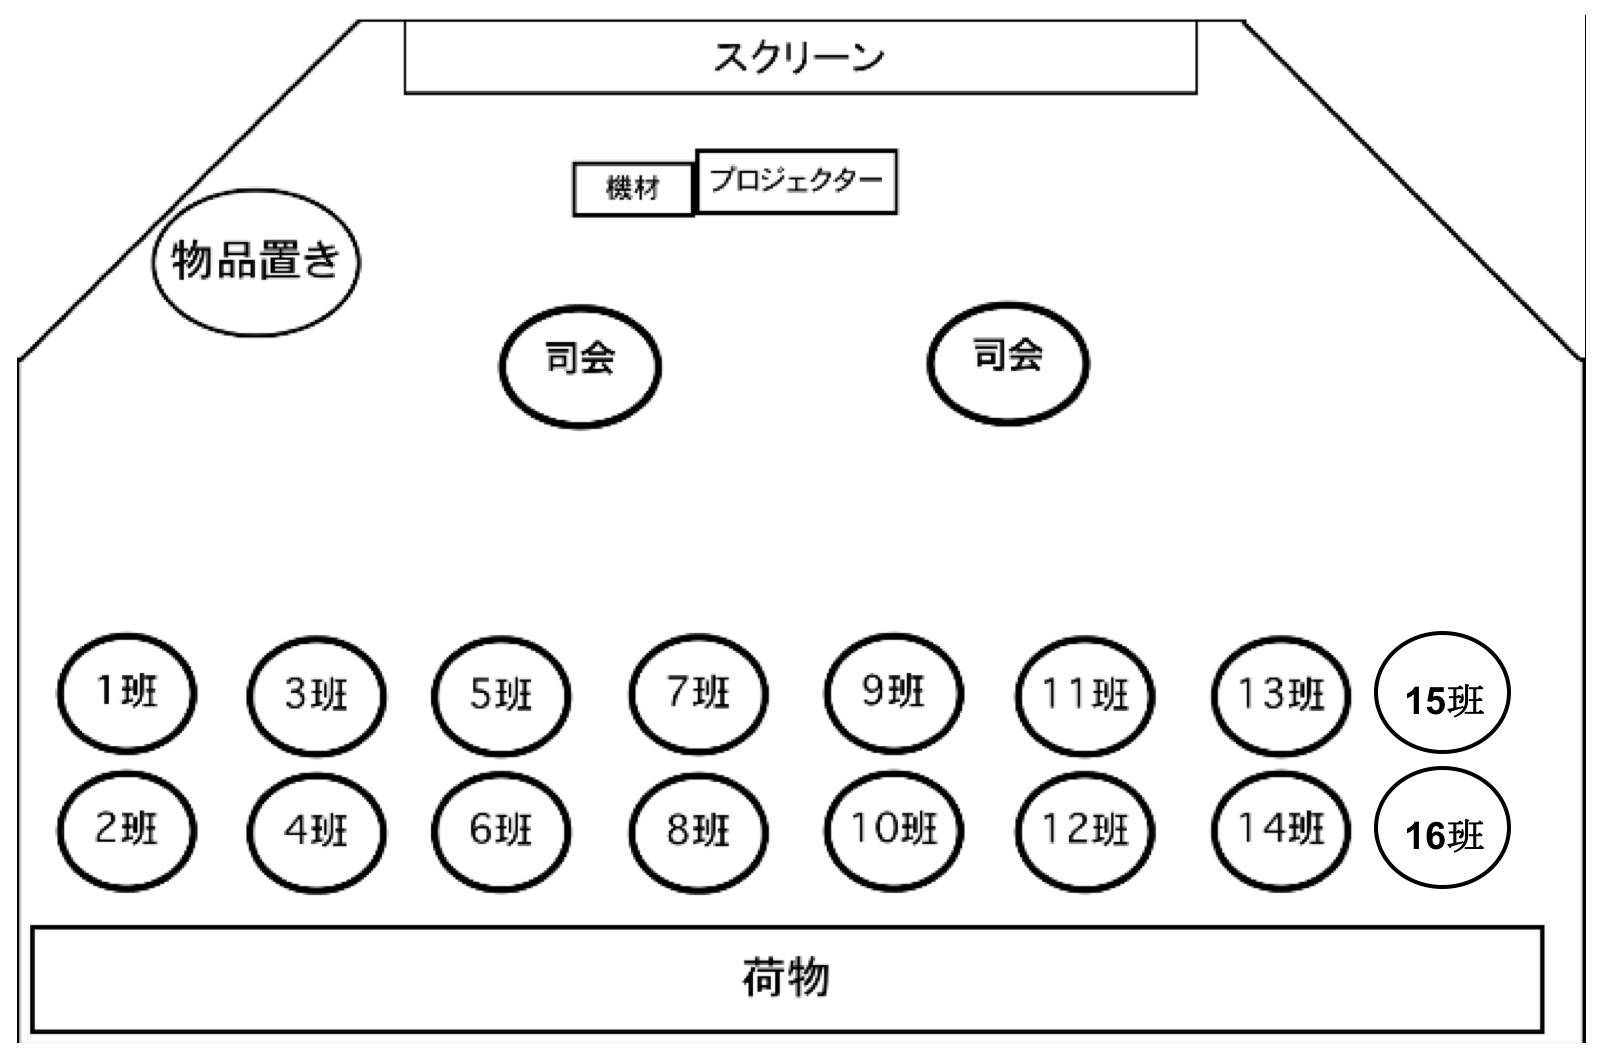
\includegraphics[scale=0.5]{./21/ice.eps}
    \caption{アイスブレイクの全体配置}
    \label{fig:ice}
  \end{center}
\end{figure}


% イベントに必要な物品と個数を記入する
% 記入例 ・マジックペン 10本
\subsection{必要物品}
\begin{itemize}
\item マイク(司会用)3本
\item スピーカー 2台
\item プロジェクタ 1台
\item 長机(プロジェクタ設置用) 1台
\item 椅子(機器操作用) 1脚
\item スクリーン 1台
\item ノートパソコン 1台
\item お題が書かれた紙(10枚程度)が入った封筒 16班1セット
\end{itemize}


% 注意事項やスタッフに周知しておくべきことがあれば記入する
\subsection{備考}
時間が短いので手早い行動を心掛けて下さい.

%\include{end}

\end{document}

\include{./22/22seikatusyokai}
% --*- coding:utf-8-unix mode:latex -*--
%\include{begin}
%%%%%%%%%%%%%%%%%%%%%%%%%%%%%%%%%%%%%%%%%%%%%%%%%%%%%%%%%%%%%%%%%%%%%%%%%%%%%%%

\section{退所式}

\subsection{日時・場所}
\begin{tabular}{p{2zw}rp{38zw}}
  日時 & : & 2019年4月6日(土) 11:25 $\sim$ 11:55\\
  場所 & : & 体育館
\end{tabular}

\subsection{タイムスケジュール}
% 時刻は必ず4桁(00:00)で書くこと!!!
\begin{longtable}{p{3zw}p{39zw}}
  11:25 & \textbf{◎ トイレ休憩} \\
        & \ \ \textbullet \ \ 司会(生野,貞松)はトイレ休憩のアナウンスを行う\\
        & \ \ \textbullet \ \ ペーパードミノの点数集計結果を小島に伝え,小島がパワーポイントに反映する\\
        & \ \ \textbullet \ \ 司会者は整列をするように促す\\
        & \ \ \textbullet \ \ 各班のスタッフはプラカードを持ち一列に整列させ,全員が揃った班はその場に座る \\\\
        & \ \ \textbullet \ \ 日下は幡多職員に退所挨拶のお願いと記念撮影のお願いをするために,事務室に行く \\\\

  11:40 & \textbf{◎ Flying Fish斉唱} \\
  	& \ \ \textbullet \ \ 小島はFlying Fishを流す \\\\

  11:46 & \textbf{◎ 代表挨拶)} \\
	& \ \ \textbullet \ \ 司会は代表(宮尾)にマイクを渡す \\\\

  11:48 & \textbf{◎ 幡多職員による挨拶} \\
  	& \ \ \textbullet \ \ 宮尾は幡多職員にマイクを渡す \\
  	& \ \ \textbullet \ \ 挨拶が終わり次第,宮尾はマイクを受け取る \\\\

  11:50 & \textbf{◎ 記念撮影} \\
	& \ \ \textbullet \ \ 幡多職員に記念撮影を行ってもらう \\
        & \ \ \textbullet \ \ 体育館の2階から撮影し,司会(もしくは近くのスタッフ)は全員を列をできるだけ崩さないように集まることを促す \\
  & \ \ \textbullet \ \ 記念撮影が終わり次第,撮影前の並びに戻るよう誘導し、元の体形に戻る \\\\

  11:55 & \textbf{◎ 退所式終了} \\
\end{longtable}

\subsection{人員配置}
\begin{itemize}
\item 司会:新川,貞松
%\item 景品授与担当:南部,松尾,半田,かりん
\item 幡多職員にお願いに行く係:日下
\item 機材係・音響係:小島
\item 集計係:小島
%\item 写真撮影 : 〇〇
\end{itemize}


\subsection{必要物品}
\begin{itemize}
\item ワイヤレスマイク:2個
\item スピーカー:2個
\item 机:1つ
\item PC
\item プロジェクタ:2台(1台は幡多)
\item 記念撮影用カメラ
\item Flying Fish音源
\item プラカード
\end{itemize}
\subsection{備考}
\begin{itemize}
\item 写真撮影を頼むために職員さんに残って欲しい旨を伝える
\end{itemize}

\subsection{全体配置}
\begin{figure}[htbp]
  \begin{center}
  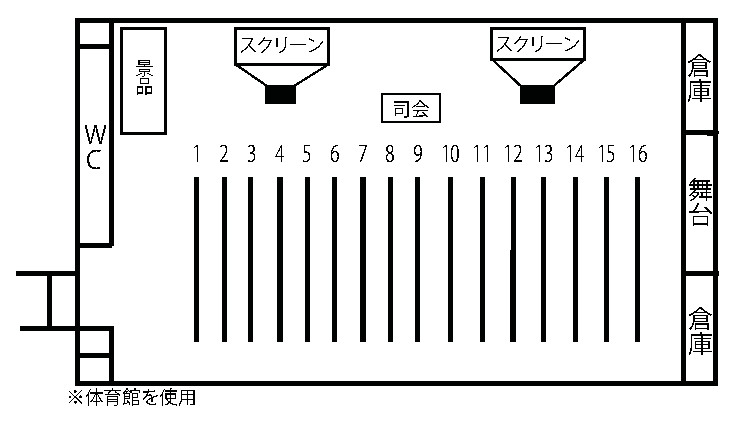
\includegraphics[width = 15cm]{./24/hyousyou.eps}
  \caption{退所式}
  \end{center}
\end{figure}

%%%%%%%%%%%%%%%%%%%%%%%%%%%%%%%%%%%%%%%%%%%%%%%%%%%%%%%%%%%%%%%%%%%%%%%%%%%%%%%
%\include{end}

% --*- coding:utf-8-unix mode:latex -*--
%\include{begin}
%%%%%%%%%%%%%%%%%%%%%%%%%%%%%%%%%%%%%%%%%%%%%%%%%%%%%%%%%%%%%%%%%%%%%%%%%%%%%%%

\section{昼食}

\subsection{日時・場所}
\begin{tabular}{p{2zw}rp{38zw}}
  日時 & : & 2019年4月6日(土) 11:55 $\sim$ 13:15 \\
  場所 & : & 食堂
\end{tabular}


\subsection{タイムスケジュール}
% 時刻は必ず4桁(00:00)で書くこと!!!
\begin{longtable}{p{3zw}p{39zw}}
  11:55 & \textbf{◎ 食堂への移動・体育館の片付け} \\
        & \ \ \textbullet \ \ 記念撮影終了後,代表(宮尾)が昼食を食堂で食べることを伝え、スタッフは新入生を連れて,4,5班ずつ食堂へと移動する \\
        & \ \ \textbullet \ \ 先遣隊と後遣隊は,体育館に戻り片付けをし,終わり次第食堂で昼食を食べる \\
        & \ \ \textbullet \ \ 食堂内誘導係(日下,堀川)は退所式が終わったら,素早く食堂へ向かう \\
        & \ \ \textbullet \ \ 食堂内誘導係(日下,堀川)はバスの号車ごとに座る場所を伝える \\
        & \ \ \textbullet \ \ 手の空いているスタッフは,食堂に着いたら奥から詰めて座ることを伝える \\
        & \ \ \textbullet \ \ 最後に新入生を誘導してきたスタッフは食堂に着いたことを食堂内誘導係の人に伝える \\

  12:00 & \ \ \textbullet \ \ 食堂で昼食をとる \\
        & \ \ \textbullet \ \ 食べ終わった人は食堂で待機する \\
        & \ \ \textbullet \ \ バス司会者(塩谷, 中島, 丸田, 高橋, 北村, 藤田)は早めに昼食を済ませ,周辺で待機しておく \\
        & \ \ \textbullet \ \ トイレ係(日下,堀川)はなるべく出入り口に近い位置で昼食をとる \\
        & \ \ \textbullet \ \ トイレ係は食堂から出入りする新入生を見張る \\

  12:30 & \textbf{◎ バス到着予定} \\
        & \ \ \textbullet \ \ バス(運転手:???,???, ???)が到着するのでバス司会は周辺で待機する \\\\

  13:10 & \textbf{◎ バス出発準備アナウンス} \\
        & \ \ \textbullet \ \ 食堂内案内係(日下,堀川)は食器を片付け,トイレを済ませておくようにアナウンスする \\
        & \ \ \textbullet \ \ 食堂内案内係(日下,堀川)はトイレに行きたくなった新入生を見張る \\
        & \ \ \textbullet \ \ 東は,たばこ吸いに行っている先生方に出発の時間が近づいていることを知らせる \\
        & \ \ \textbullet \ \ バス司会からバス到着の連絡が来たら,小谷は事務室に行って鍵を開けてもう\\
        & \ \ \textbullet \ \ バス司会1(藤田,中島,丸田)は食堂から第一・二研修室,バスへ誘導案内する \\
        & \ \ \textbullet \ \ スタッフは新入生の誘導の補助をしながら第一・二研修室へ荷物を取りに行き,バスへ向かう \\
        & \ \ \textbullet \ \ 日下は全員が食堂を出たら,食堂内に忘れ物がないかを確認し,バスへ向かう \\
        & \ \ \textbullet \ \ バス司会者2(北村,高橋(龍),塩谷)はバスに乗り込む新入生のチェックをする \\
        & \ \ \textbullet \ \ 各号車に乗るスタッフは,新入生と先生の荷物の積みこむ \\
  \end{longtable}

\newpage

\subsection{人員配置}
\begin{itemize}
\item 食堂内案内係:日下,堀川
\item 体育館の片付け:先遣隊,後遣
\item 新入生・先生誘導係:各班のイベントスタッフ
\item タバコを吸いに行っている先生方へ出発の知らせをする係:東
\item バス司会1:藤田,丸田,中島
\item バス司会2:北村,高橋(龍),塩谷
\end{itemize}


\subsection{必要物品}
乗車確認リスト:3部


\subsection{備考}
\begin{itemize}
  %\item 各班食べ終わった弁当はまとめておく、班全員が食べ終わったら配布された場所に持っていく
  %\item トイレに行きたい人は体育館のトイレに行くように誘導する
  \item 食事はついた人から号車ごとに奥から座って食べる
  \item 移動後トイレに行きたい人は食堂近くのトイレに行くようにスタッフが誘導する
  %\item は第一集会室から全員の荷物がなくなったら,第一集会室の鍵を閉め,持っている鍵を室戸事務室に返却する
\end{itemize}




%%%%%%%%%%%%%%%%%%%%%%%%%%%%%%%%%%%%%%%%%%%%%%%%%%%%%%%%%%%%%%%%%%%%%%%%%%%%%%%
%\include{end}

%\include{begin}

\section{バス内(帰り)}

\begin{tabular}{p{2zw}rp{38zw}}
  日時 & : & 2019年4月6日(土) 13:30 $\sim$ 16:00\\
  場所 & : & バス内
\end{tabular}

\subsection{目的}
新入生と一緒に二日間を振り返り,共感しあう.

%\subsection{イベント内容}

\subsection{タイムスケジュール}
% 時刻は必ず4桁(00:00)で書くこと!!!
\begin{longtable}{p{3zw}p{39zw}}
  %%14:05 & \textbf{◎ 幡多青少年自然の家出発} \\
  13:30 & \textbf{◎ 幡多少年自然の家出発} \\
        & \ \ \textbullet \ \ 司会者が二日間の感想を話す(野外炊事やイベント,就寝の時の話など)  \\
        & \ \ \textbullet \ \ 新入生に感想などを聞いてみる(新入生が疲れているようなら控えておく) \\
        & \ \ \textbullet \ \ あぐり窪川到着予定時刻とトイレについて話し,後はフリーな時間とする \\\\

  %%14:50 & \textbf{◎ あぐり窪川到着5分前} \\
  14:15 & \textbf{◎ あぐり窪川到着5分前} \\
        & \ \ \textbullet \ \ トイレについての説明と,5分前に集合することを話す(行きと同じ)  \\\\

  %%14:55 & \textbf{◎安芸駅(安芸球場)到着} \\
  14:20 & \textbf{◎安芸駅(安芸球場)到着} \\
        & \ \ \textbullet \ \ 休憩時間を伝える\\
        & \ \ \textbullet \ \ 到着の旨を報告LINEで連絡する \\\\

  %%15:10 & \textbf{◎ あぐり窪川出発5分前} \\
  14:35 & \textbf{◎ あぐり窪川出発5分前} \\
        & \ \ \textbullet \ \ 司会者が人数チェックする(行きと同様に行う)\\\\


  %%15:15 & \textbf{◎ あぐり窪川出発} \\
  14:40 & \textbf{◎ あぐり窪川出発} \\
	& \ \ \textbullet \ \ 工科大到着時刻と到着後各自解散することを伝える\\
	& \ \ \textbullet \ \ 出発の旨を報告LINEで連絡する\\\\


  %%16:00 & \textbf{◎ 工科大到着5分前} \\
  15:55 & \textbf{◎ 工科大到着5分前} \\
      	& \ \ \textbullet \ \ 工科大到着後荷物を持ち,流れ解散であることを伝える \\
        & \ \ \textbullet \ \ 降車の際,名札を回収することを伝える\\
        & \ \ \textbullet \ \ 忘れ物がないように伝える\\
        & \ \ \textbullet \ \ 最後に司会者が締めくくる\\\\

  %%16:05 & \textbf{◎ 工科大到着} \\
  16:00 & \textbf{◎ 工科大到着} \\
        & \ \ \textbullet \ \ 到着の旨を報告LINEで連絡する\\
        & \ \ \textbullet \ \ 最初に補助席に座っているスタッフが降車する\\
        & \ \ \textbullet \ \ 降車したスタッフは乗降口で名札を回収する(しおりは各自持ち帰ってもらう)\\
        & \ \ \textbullet \ \ 残りのスタッフは荷物を降ろす\\
        & \ \ \textbullet \ \ 新入生に挨拶をし,見送る(最後の新入生が帰り次第終了する)\\
        & \ \ \textbullet \ \ 新入生が完全に解散した旨を報告LINEで連絡する\\
        & \ \ \textbullet \ \ 司会は忘れ物が無いか確認する \\
        & \ \ \textbullet \ \ 記念撮影  \\
\end{longtable}


\subsection{人員配置} %未定
○ 1号車
\begin{itemize}
\item 司会:東,江川
\item 1号車受付:石野
\item 補助:横田,別役
\end{itemize}

○ 2号車
\begin{itemize}
\item 司会:宮尾,以西
\item 2号車受付:南部
\item 補助:藤沢,高島
\end{itemize}

○ 3号車
\begin{itemize}
\item 司会:真壁,渡辺
\item 3号車受付:藤田(竜世)
\item 補助:松尾,小谷
\end{itemize}

◯ 救護車
\begin{itemize}
\item 藤田(竜貴), 角原, 小松
\end{itemize}

\subsection{必要物品}
\begin{itemize}
\item 酔い止め薬:各バス1箱
\item エチケット袋:各バス2枚
\item 紙コップ:各バス5個
\item 水(常温):各バス500ml 1本
\item 名札回収用袋:3つ
\end{itemize}


\subsection{備考}


%\include{end}

% 必要な項目ができた場合は適宜サブセクションを追加してください

%\include{begin}

% イベント名を記入する
\section{片付け(体育館)}
% 日時と場所を記入する
% 時刻は4桁で記入すること!
\subsection{日時・場所}
\begin{tabular}{p{2zw}rp{38zw}}
  日時 & : & 2019年4月6日(土) 11:55(イベントが終わり次第) $\sim$\\
  場所 & : & 体育館
\end{tabular}

% 目的を記入する
\subsection{目的}
先遣隊と後遣隊のメンバーが掃除する。来た時よりも美しく。

% イベントの概要やルールを記入する

% イベントのタイムスケジュールを記入する
% 時刻は必ず4桁(00:00)で記入すること!
% 時間の流れは途切れないように記述する!
\subsection{タイムスケジュール}
\begin{longtable}{p{3zw}p{39zw}}
  11:55 & \textbf{◎ 作業} \\
  		& \ \  \textbullet \ \ 昼食が終わり次第片付けを行う \\
        & \ \  \textbullet \ \ 小松,小島,西森は車を正面広間に移動する \\
        & \ \  \textbullet \ \ 横田は体育館,野田,以西は各研修室の持って帰る荷物とゴミを片付ける \\
        & \ \  \textbullet \ \ 片付けの際は宴用の余ったゴミ袋を使用。余らなかった場合は幡多の職員にゴミ袋をもらってくる \\
        & \ \  \textbullet \ \ 小松, 小島, 西森は車を移動したあと片付けに参加する \\
        & \ \  \textbullet \ \ 新入生が食堂からバスに移動するまでに机と椅子の片付けを行う \\\\
        
        & \ \  \textbullet \ \ 片付けが終了次第,食堂へ移動し昼食をとる \\\\
        
  
  13:10 & \textbf{◎ 昼食・幡多出発} \\
        & \ \  \textbullet \ \ 昼食を食べ終わり次第,片付け,忘れ物などをチェックする \\
        & \ \  \textbullet \ \ 全ての片付け終了後,幡多を出発する \\
\end{longtable}


% イベントに必要な役割と人数を記入する
% 担当者は決定次第追記する
% 記入例 ・司会者 2人(名前1、名前2)
\subsection{人員配置}
\begin{itemize}
\item 先遣隊:宮尾,小松,小島,横田,野田,以西
\item 後遣隊:西森,藤沢
\end{itemize}


% イベントを実施するときに新入生や先生、スタッフがどこに配置するかを記入する
% 図があるとわかりやすい
%\subsection{車の停車位置}
%\begin{figure}[h]
% \begin{center}
%  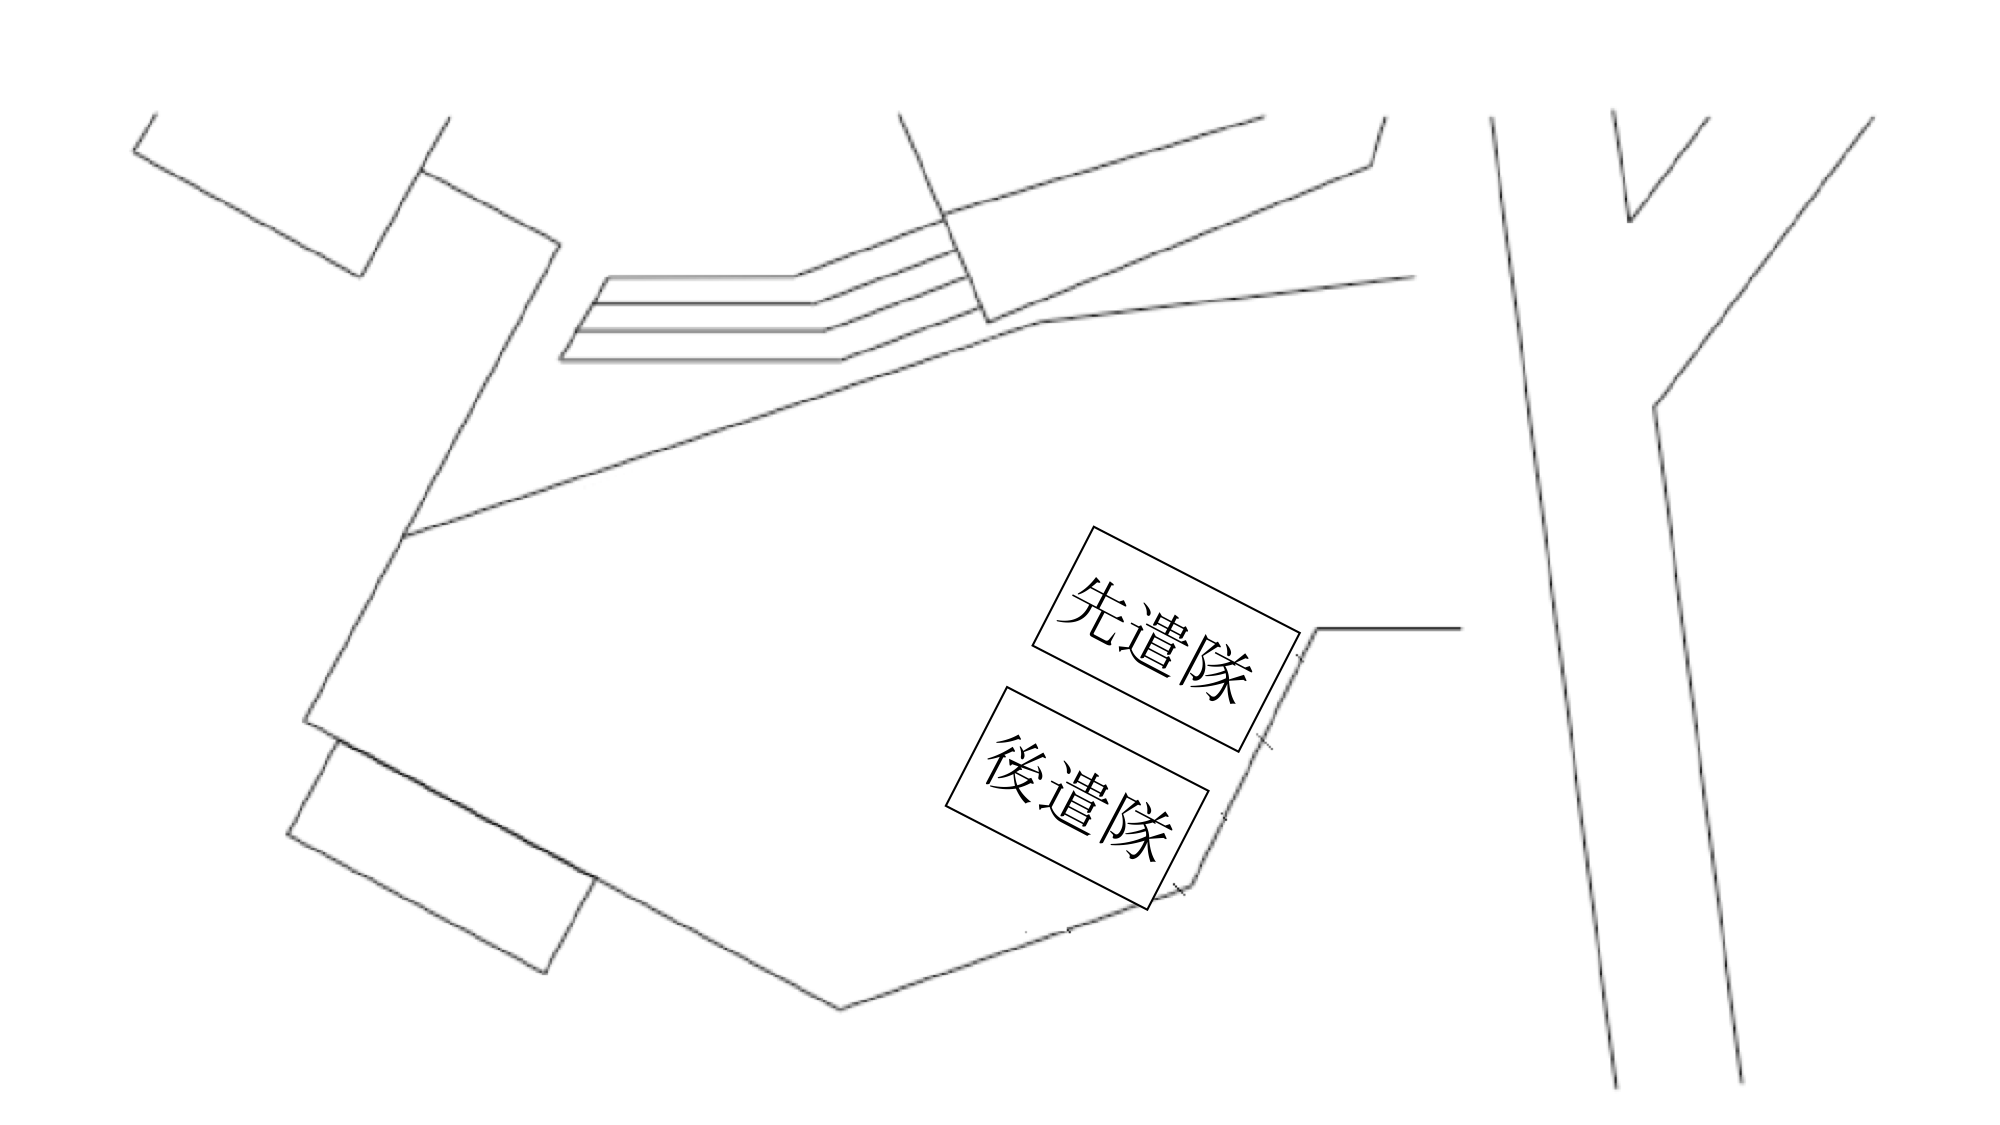
\includegraphics[width=115mm,height=70mm]{./27/syomenhiromacar.eps}
% \end{center}
% \caption{駐車場車配置}
%\end{figure}

\subsection{必要物品}
\begin{itemize}
\item 業務用ゴミ袋
\end{itemize}


\subsection{備考}
\begin{itemize}
\item ゴミは分別する
\item 机,椅子等の施設用具は幡多職員に片付ける場所を確認しておく
\item 忘れ物を入念にチェックする
\end{itemize}


%\include{end}


% 必要な項目ができた場合は適宜サブセクションを追加してください

%\include{begin}

% イベント名を記入する
\section{大学到着後}


% 日時と場所を記入する
% 時刻は4桁で記入すること!
\subsection{日時・場所}
\begin{tabular}{p{2zw}rp{38zw}}
  日時 & : & 2019年4月6日(土) 16:00 $\sim$\\
  場所 & : & 東ロータリー,????
\end{tabular}


% イベントのタイムスケジュールを記入する
% 時刻は必ず4桁(00:00)で記入すること!
% 時間の流れは途切れないように記述する!
\subsection{タイムスケジュール}
\begin{longtable}{p{3zw}p{39zw}}
  16:00 & \textbf{◎ 工科大到着} \\\\

  16:15 & \textbf{◎ 新入生見送り終了} \\
        & \ \ \textbullet \ \ 新入生全員の解散の確認後,スタッフの荷物,その他物品を????に全員で運ぶ \\\\

  16:20 & \textbf{◎ 集合写真撮影} \\
        & \ \ \textbullet \ \ 新入生を見送り次第,スタッフ全員で集合写真を撮る \\
        & \ \ \textbullet \ \ 撮影者は栗原先生にやっていただく \\

  16:25 & \textbf{◎ 教室移動後}  \\
        & \ \ \textbullet \ \ 先遣隊,後遣隊はゴミを指定の場所へ捨てに行く \\
        & \ \ \textbullet \ \ 分別ができていないものは分別する \\
        & \ \ \textbullet \ \ 各研究室,個人,教務部から借りた物品が揃っていることを確認し,順次返却を行う(教務部への返却は???,???が行う) \\
        & \ \ \textbullet \ \ 返却先が不在等で返却できない場合,一時的に???研究室にて荷物を保管しておき,後日代表陣が物品の返却を行う \\\\

  16:40 & \textbf{◎ 反省会} \\\\

  17:00 & \textbf{◎ 解散!!} \\
\end{longtable}

\subsection{人員配置}
教務部への物品返却:?松本,藤田(竜貴)

% イベントに必要な物品と個数を記入する
% 記入例 ・マジックペン 10本
\subsection{必要物品}
物品用チェックリスト


% 注意事項やスタッフに周知しておくべきことがあれば記入する
\subsection{備考}
スタッフの皆さん本当にお疲れ様でした.そして,ありがとうございました.帰ってゆっくりと体を休めてください.後日,打ち上げがあるので是非参加してくださいね.打ち上げで会いましょう!

%\include{end}



\end{document}
